\chapter{Results - Person specific}
{\samenvatting This section explains the results found in a person specific setting. It starts by explaining the used approach before proceeding with a performance comparison of the different classifiers. Next the certainty of the classifiers is investigated, combined with the selected features and EEG channels. This chapters end with a discussion about the stability of the different methods.}

\section{Used approach}
\label{approach}

The first part of this work is looking at features in a person specific setting. This means that the algorithm is trained and tested on data from the same person. The main goal was to find features that give insight in the arousal and valence state of a person. This was done by comparing the aforementioned features and feature selection methods. For this a two stepped algorithm, inspired by the advanced random forest method, explained in Section \ref{rfmethod}, was used. In short, the first step is to rank all the features and only take the top X of the features. This threshold is applied to limit computation times and cancel features with low or zero importance. The next step is to build a model by selecting features out of the remaining feature set. This approach is depicted in Figure \ref{flow}.

\mijnfiguur{width=0.9\textwidth}{flow}{The used approach of this thesis.}

As you can see in Figure \ref{flow}, the approach starts by separating a test set to evaluate the final performance of the algorithm. This test set contains 10 of the 40 samples. Next, the aforementioned feature selection methods are applied to the train set. A top $X$ of the features is then kept, all other features are cancelled.

\npar

In the next step a model is build with the selected features. This is done iteratively by starting with an empty feature set. In the add step, a feature is added to this set and the cross validation error is determined. This step is important because it ensures that chosen features have good generalisation properties. Next the average of the cross validation errors and the standard deviation is calculated. The average cross validation minus the standard deviation is then compared to the previous best performance. If the performance is better, the feature is kept in the feature set. If the performance is not better, the feature is neglected. This is repeated for all the features and is known as greedy forward selection in literature \citep{greedyFS}. The standard deviation is included to increase the stability of the algorithm, by avoiding that small differences in averages lead to a different model. This was used rather than a statistical test, as it already provided good results in the original algorithm\ref{rfmethod}.

\npar

In the final step the performance of the test set is determined by the accuracy metric. Accuracy is chosen as metric, because this metric gives a clear and intuitive measurement of performance.

\npar

The first parameter of this flow is the threshold parameter, indicated in the figure as $X$. This threshold cancels features with low importance, by simply taking the best $X$ features from the feature ranking. Assigning a high value to the threshold will increase calculation times as more features are available for the building phase. The performance of the model, will not be better though. Most of the additional features will have low importance values and are not likely to improve performance. Setting a low threshold might cancel out important features. 
In this work, the threshold parameter was fixed to 30 for all feature selection methods for the following two reasons. First, considering that there are 30 samples in the feature set, having 30 features is already more than enough. Note that a well-known rule of thumb is to have at least 10 times more samples than features\citep{rot1,rot2}\footnote{Note that this is just a rule of thumb, and therefore not proven theoretically. In practice however, it turns out to work quite well.}. Second, looking at the features that were selected during training, one can see that usually around 5-7 features remain. The last selected feature usually has a rank around 20, meaning that the last 10 available features in the building phase are rarely used.

\npar
A second parameter of this model is a model to estimate the performance. For this, an SVM with a radial basis functions (RBF) kernel is used as model. This model was chosen because it has proven itself in multiple emotion recognition studies\citep{killyPaper,emorecoghard,SVMUsage,SVMUsage2}. SVMs look for a separation boundary between two classes, and thus only look at points close to that boundary. This gives this method an advantage in this experiment, as the dataset only contains 40 samples for each person, only 30 of them are available for training. Another advantage of the marginalization maximization and the regularization is that SVMs are capable of handling large features sets\citep{SVMLargeFeatSets,SVMLargeFeatSets2}, which concurs with this work's problem statement.

\npar

Some feature selection methods use a machine learning technique as basis. These methods were not used in the final building phase. This was done because some underlying methods are actually regression algorithms, meaning that they will produce a continuous output. This is in contrast with the classification problem that is solved in this work\footnote{Several tests in the early stage of this work indicated that even though continuous valence and arousal values are available, classification was more designated. The current state of the art emotion recognition systems is still limited to classification, because regression proves to be a difficult problem. One possible reason for this might be that each person has his/her own interpretation of the valence / arousal scales. A positive feeling with valence level 6 of one person does not correspond to the exact same feeling of another person.}. To ensure that all final models were capable of classification, one classification model was used in the final step. This ensures that the comparison between feature selection methods was possible.

\section{Performance}

When looking at the accuracies of different feature selection models in combination with the SVM, it is clear that there is not a lot of difference. For each feature selection method, the test accuracy and standard deviation are shown in Table \ref{accCompLblarousal} and Table \ref{accCompLblvalence} for valence and arousal respectively. The accuracies are also plotted in in Figure \ref{accComp_arousalSVM} and Figure \ref{accComp_valenceSVM} for arousal and valence respectively. Scores for each person can be found in Appendix \ref{persScores}.

\mijnfiguur{width=1.\textwidth}{accComp_arousalSVM}{Comparison of different feature selection methods for arousal recognition. The y-axis shows the test accuracy averages over all persons as well as the standard deviation. The x-axis shows the different models, each number corresponds to the number in Table \ref{accCompLblarousal}. Blue bars correspond to filter selection methods, red bars correspond to wrapper methods and green bars are used for the embedded methods.}

\begin{table}[H]
\centering
\caption{A comparison of the accuracy of different feature selection methods for arousal. The reported scores are test accuracies averaged over the different persons with their standard deviation.\label{accCompLblarousal}.}
\begin{tabular}{llll}
\textbf{Number} & \textbf{Feature selection method} & \textbf{Avg test acc - arousal} & \textbf{Std test acc - arousal} \\ \hline
0               & pearson                           & 0.68125                             & 0.1615199978                    \\
1               & mutual information                & 0.571875                            & 0.1708316942                    \\
2               & distance correlation              & \textbf{0.709375}                   & \textbf{0.1201058001}           \\
3               & ANOVA                             & 0.659375                            & 0.1701221098                    \\
4               & linear regression                 & 0.640625                            & 0.1477997228                    \\
5               & SVM                               & 0.671875                            & 0.1570583927                    \\
6               & LDA                               & 0.634375                            & 0.138212961                     \\
7               & lasso regression                  & 0.70625                             & 0.1435438564                    \\
8               & ridge regression                  & 0.653125                            & 0.1436491582                    \\
9               & random forests                    & \textbf{0.7}                        & \textbf{0.1391216687}           \\
10              & PCA                               & 0.578125                            & 0.1518368713                   
\end{tabular}
\end{table}

\mijnfiguur{width=1.\textwidth}{accComp_valenceSVM}{Comparison of different feature selection methods for valence recognition. The y-axis shows the test accuracy averages over all persons as well as the standard deviation. The x-axis shows the different models, each number corresponds to the number in Table \ref{accCompLblvalence}. Blue bars correspond to filter selection methods, red bars correspond to wrapper methods and green bars are used for the embedded methods.}

\begin{table}[H]
\centering
\caption{A comparison of the accuracy of different feature selection methods for valence. The reported scores are test accuracies averaged over the different persons with their standard deviation.\label{accCompLblvalence}}
\begin{tabular}{llll}
\textbf{Number} & \textbf{Feature selection method} & \textbf{Avg test acc - valence} & \textbf{Std test acc - valence} \\ \hline
0               & pearson                           & 0.6875                              & 0.1313699529                    \\
1               & mutual information                & 0.58125                             & 0.1446631237                    \\
2               & distance correlation              & 0.66875                             & 0.1330474085                    \\
3               & ANOVA                             & 0.703125                            & 0.133161011                     \\
4               & linear regression                 & 0.5625                              & 0.1560603688                    \\
5               & SVM                               & 0.65625                             & 0.1389766748                    \\
6               & LDA                               & 0.6125                              & 0.187943025                     \\
7               & lasso regression                  & 0.678125                            & 0.1660438632                    \\
8               & ridge regression                  & 0.575                               & 0.1436842416                    \\
9               & random forests                    & \textbf{0.7375}                     & \textbf{0.1313699529}           \\
10              & PCA                               & 0.6                                 & 0.1586231078                   
\end{tabular}
\end{table}

\section{Correlation probability and level of valence/arousal}\label{corrs}

The current model is a classification model, meaning that it divides the valence and arousal into two classes: high and low. The classes are determined by a binary separation. Both valence and arousal range between 1 and 9, so every value between 5 is regarded as a low valence/ arousal. All values above 5 are regarded as high valence/arousal.

\npar

It might be interesting to look at the prediction probability a model gives to its output and the distance of the arousal/valence level to this separation boundary. The distance to the separation boundary (sb) of an arousal/valence value v is given by:
\begin{center}
$dist_{v, sb} = | v - sb |$
\end{center}
Using simple binary classification, which simply splits the range into two, the separation boundary has value 5. A valence level 9 has thus a distance of 4.

\npar

It is expected that samples with a valence rating far from the separation boundary, e.g. 9, should be predicted with higher confidence than one with a valence rating close to the separation boundary, e.g. 5 or 6. This should be reflected in the prediction probability, i.e. a model should be more certain of valence/ arousal values that lie further away from the separation boundary. To investigate this, the Pearson correlation coefficient R between the prediction probability and the aforementioned distance to the separation boundary was calculated. These Pearson coefficients are plotted for the model build with the corresponding feature selection methods. The Pearson correlations for arousal are depicted in Figure \ref{arousal_corrs} and Figure \ref{valence_corrs} for valence. The legend combined with the precise values, can be found in Table \ref{corrsCompLbl}.

\begin{table}[H]
\centering
\caption{This table gives the Pearson R correlation coefficients between the prediction probability and the distance between the level of arousal and the separation boundary, i.e. level 9 arousal lies at a distance |9-5| = 4, while an arousal of level 7 lies at distance 2. The assumption is that larger distances are easier to recognise, and thus be predicted with a higher confidence. The correlation should thus ideally be positive\label{corrsCompLbl}.}
\begin{tabular}{llll}
\textbf{Number} & \textbf{What}        & \textbf{arousal} & \textbf{valence}  \\ \hline
0               & pearson              & 0.03797          & 0.00957  \\
1               & mutual information   & -0.09065         & 0.00805  \\
2               & distance correlation & 0.08906          & 0.01725  \\
3               & ANOVA                & 0.07880          & -0.01745 \\
4               & linear regression    & 0.05027          & 0.09465  \\
5               & SVM                  & 0.11322          & 0.02691  \\
6               & LDA                  & -0.06053         & 0.02876  \\
7               & lasso regression     & 0.05280          & 0.17024  \\
8               & ridge regression     & 0.02897          & 0.10253  \\
9               & random forests       & 0.00439          & 0.10738  \\
10              & PCA                  & 0.02182          & 0.00875 
\end{tabular}
\end{table}

\mijnfiguur{width=1.\textwidth}{arousal_corrs}{The pearson correlations between the model's prediction probability and the distance between the subject's level of arousal and the separation boundary, see Table\ref{corrsCompLbl} for more details.}

\mijnfiguur{width=1.\textwidth}{valence_corrs}{The pearson correlations between the model's prediction probability and the distance between the subject's level of valence and the separation boundary, see Table\ref{corrsCompLbl} for more details.}

Overall, the correlations are quite low. Some correlations are even negative, meaning that the model is more certain of examples that lie closer to the separation boundary. To explain why, additional research might be needed. At first sight, several explanations for this are possible:
\begin{enumerate}
\item The correlation is present, but is more complex than a simple linear correlation. As a result, the Pearson coefficient is not able to capture this correlation well.
\item The assumption that high valence and arousal values are easier to recognise is wrong. It might be possible that a high valence/arousal levels do not correspond to increased physiological responses. Future research could look at the dominance values, that indicate how strong the emotion is perceived. The dominance values are explained in Section \ref{valarrdomspace} and were neglected during this work.
\end{enumerate}

\npar

On the other hand one can observe that the correlation for valence is a little higher than the correlation for arousal. This indicates that might it be easier to recognize valence.

\section{Selected features}

To compare which features were chosen, the feature set was divided into 8 categories:
\begin{enumerate}
\item \textbf{Power features:} PSD and FE features of a single EEG channel
\item \textbf{Asymmetry features:} DASM, RASM, DCAU and RCAU features that represent a the (a)symmetry between two EEGchannels.
\item \textbf{Fractions:} Alpha/beta and fractions of different power ratios of an EEG channels.

\item \textbf{Heart rate:} the statistical values of the heart rate.
\item \textbf{Galvanic skin response:} the statistical values of the GSR, measuring perspiration.
\item \textbf{Respiration:} the statistical values of the respiration.
\item \textbf{Bloop pressure:} the statistical values of the plethysmograph, indication the person's blood pressure.
\item \textbf{Skin temp:} the statistical values of the skin temperature.
\end{enumerate} 

The results for arousal are depicted in Figure \ref{arousalpies}, the legend is shown in Figure \ref{arousalpieslegend}. In each of these plots, a pie chart is shown that gives the distribution of all the selected features for all persons combined. When looking at the different selected features for the different feature selection methods, it becomes clear that the most valuable features are the asymmetry features combined with the power features. All feature selection methods seem to agree that those two categories are most valuable. The amount of asymmetry features is always the highest, except in case of linear, mutual information and lasso regression. These methods are not very advanced, which might explain the difference. Additionally, lasso regression is very prone to noise, as explained earlier in Section \ref{lassoregression}. Overall, the most important result for both valence and arousal is therefore that in a person-specific setting, EEG features are clearly dominant over non-EEG features. The non-EEG features are rarely selected by any of the feature selection algorithms.

\npar

The conclusion for arousal is that the different feature selection methods agree mostly on what the relevant feature categories. The most import features are the asymmetry features, followed by the power features. The non-EEG features are rarely chose and do not seem to be of importance here. It is also important to note that the fractions of frequency bands are not as important as previously thought. Literature suggested that the fractions of the alpha versus the beta frequency band would give an indication for the arousal of a subject. The main argument for this was the fact that arousal measures how active a person is feeling. A large fraction of alpha and beta power means that the brain is in a relaxed state or in an active and focussed state respectively. Looking at these fractions was therefore supposed to give insight in the arousal level of a subject. These results indicate that the asymmetry and power features are more relevant. This might mean two things, either the asymmetry and power features do contain valuable information for arousal or the algorithm is overfitting on these features.

\npar

The results for valence are depicted in Figure \ref{valencepies} and the corresponding legend in Figure \ref{valencepieslegend}. The selected features are similar to the selected features for arousal recognition. The most valuable features are again the asymmetry and power features. These results were expected, as most of the emotion recognition studies agree that the asymmetry features give insight in the valence level of a subject.

\clearpage
\begin{figure}[!tbp]
  \centering
  \begin{subfigure}[b]{0.3\textwidth}
    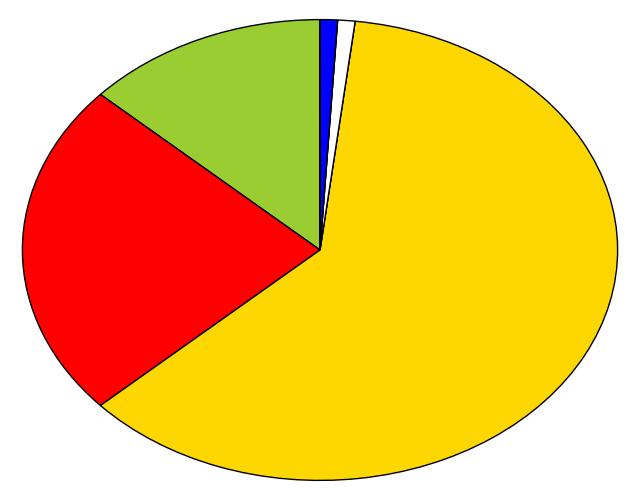
\includegraphics[width=\textwidth]{arousalALLpearsonR}
    \caption{Pearson correlation}
  \end{subfigure}
  \hfill
  \begin{subfigure}[b]{0.3\textwidth}
    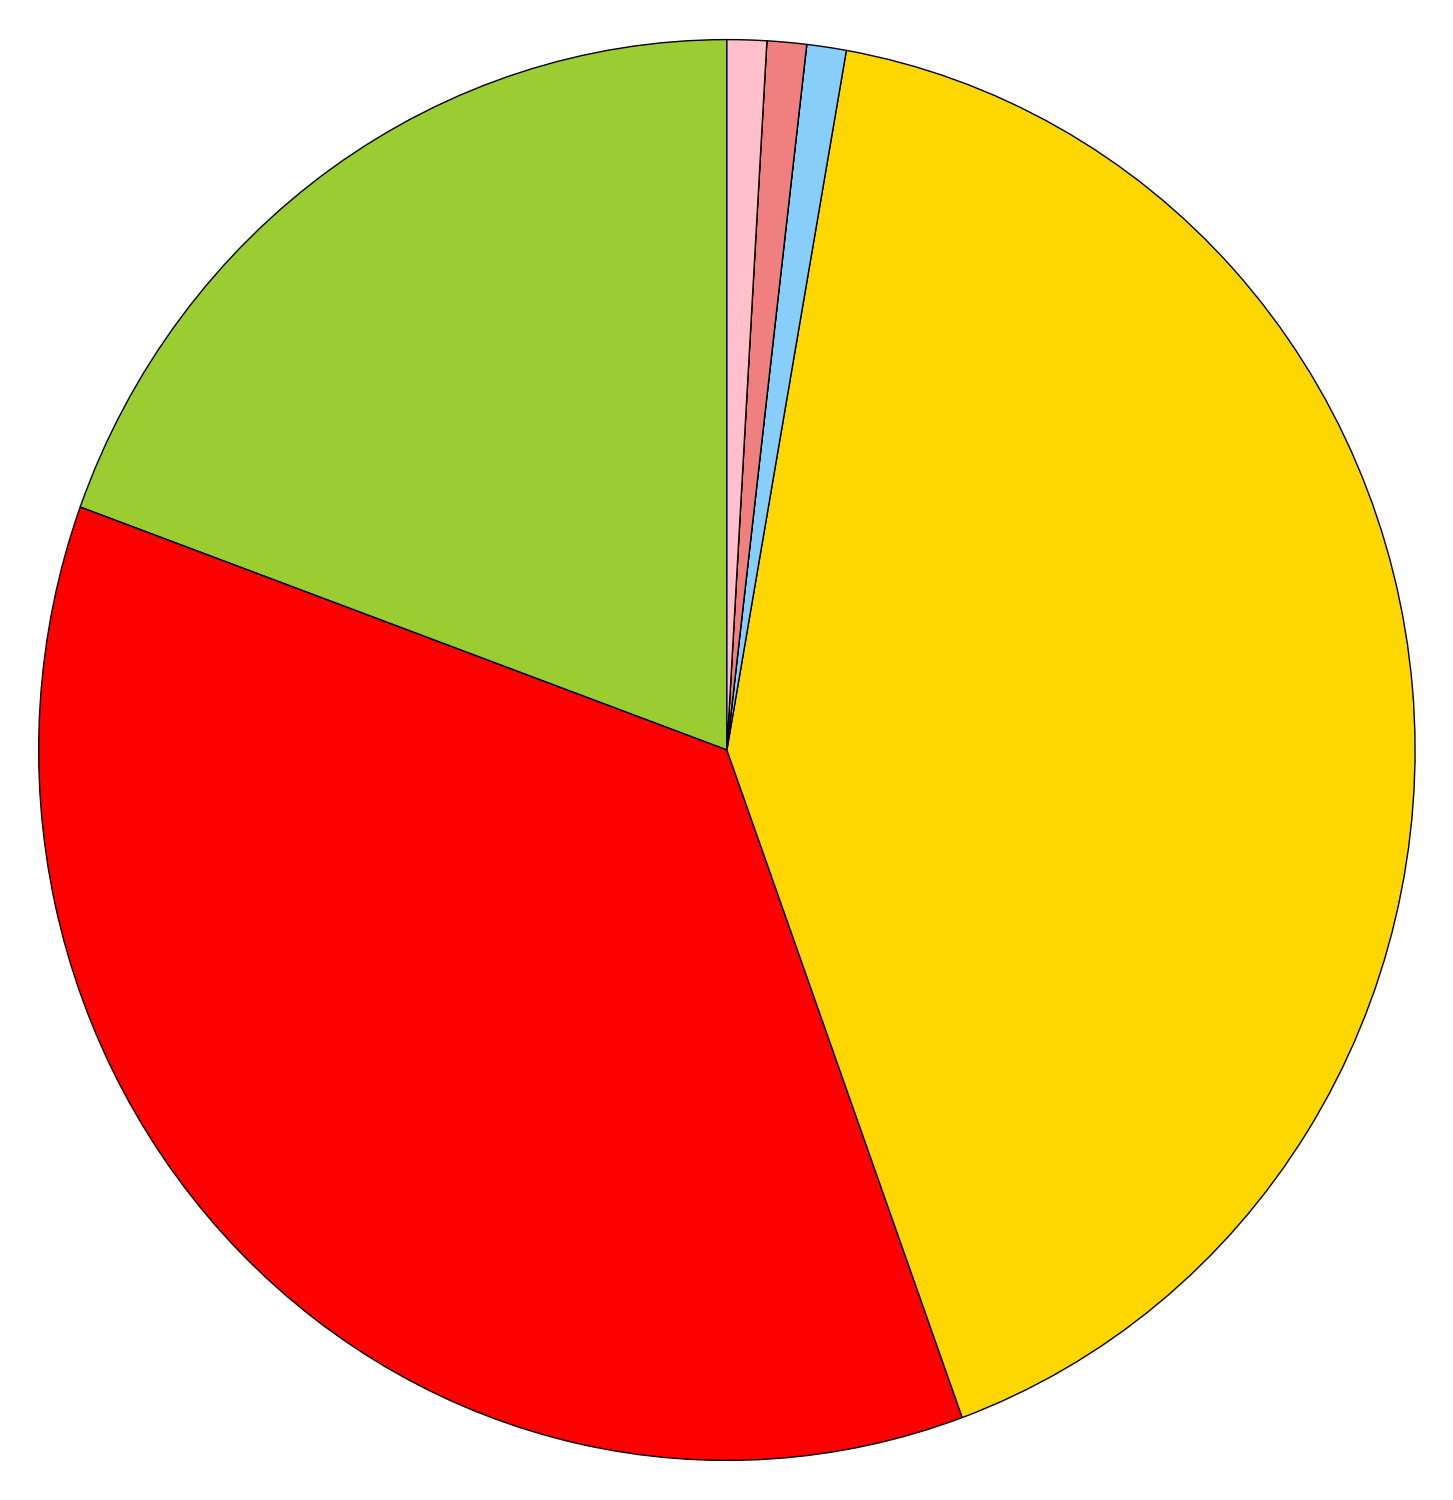
\includegraphics[width=\textwidth]{arousalALLMutInf}
    \caption{Mutual information}
  \end{subfigure}
  \hfill
  \begin{subfigure}[b]{0.3\textwidth}
    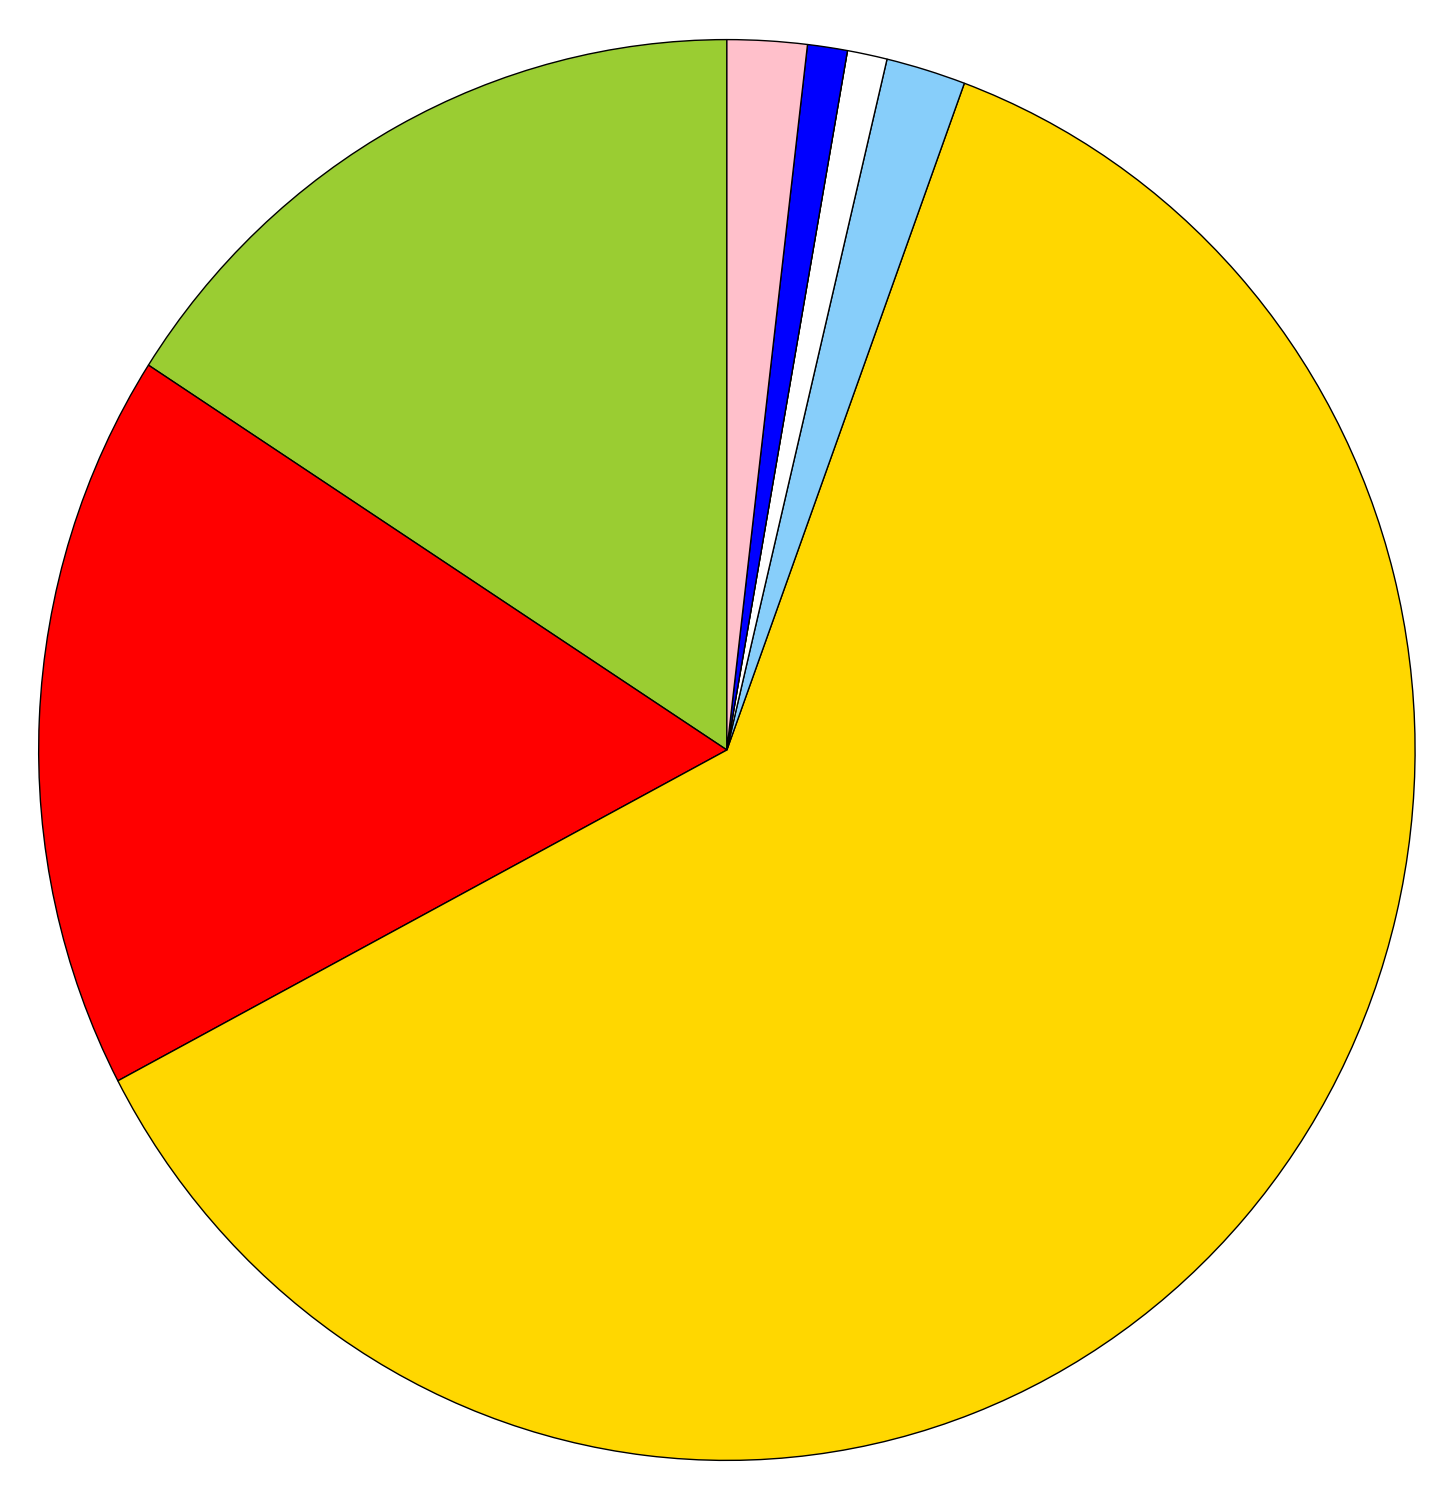
\includegraphics[width=\textwidth]{arousalALLdCorr}
    \caption{Distance Correlation}
  \end{subfigure}
  
  \begin{subfigure}[b]{0.3\textwidth}
    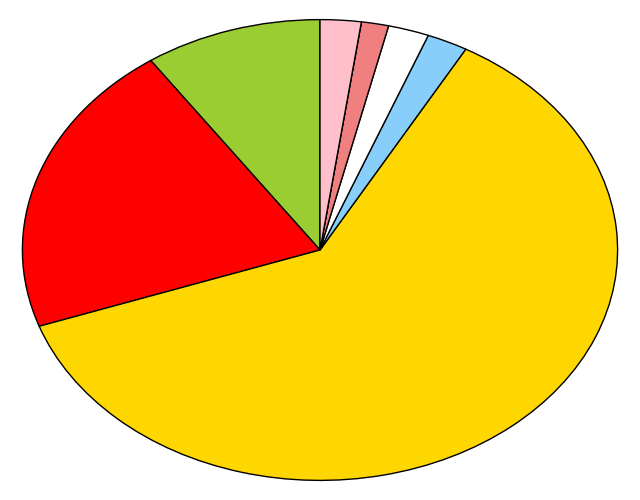
\includegraphics[width=\textwidth]{arousalALLANOVA}
    \caption{ANOVA}
  \end{subfigure}
  \hfill
  \begin{subfigure}[b]{0.3\textwidth}
    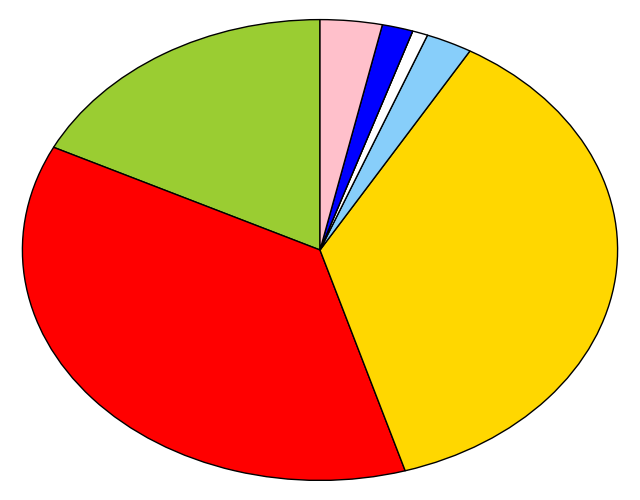
\includegraphics[width=\textwidth]{arousalALLLR}
    \caption{Linear regression}
  \end{subfigure}
  \hfill
  \begin{subfigure}[b]{0.3\textwidth}
    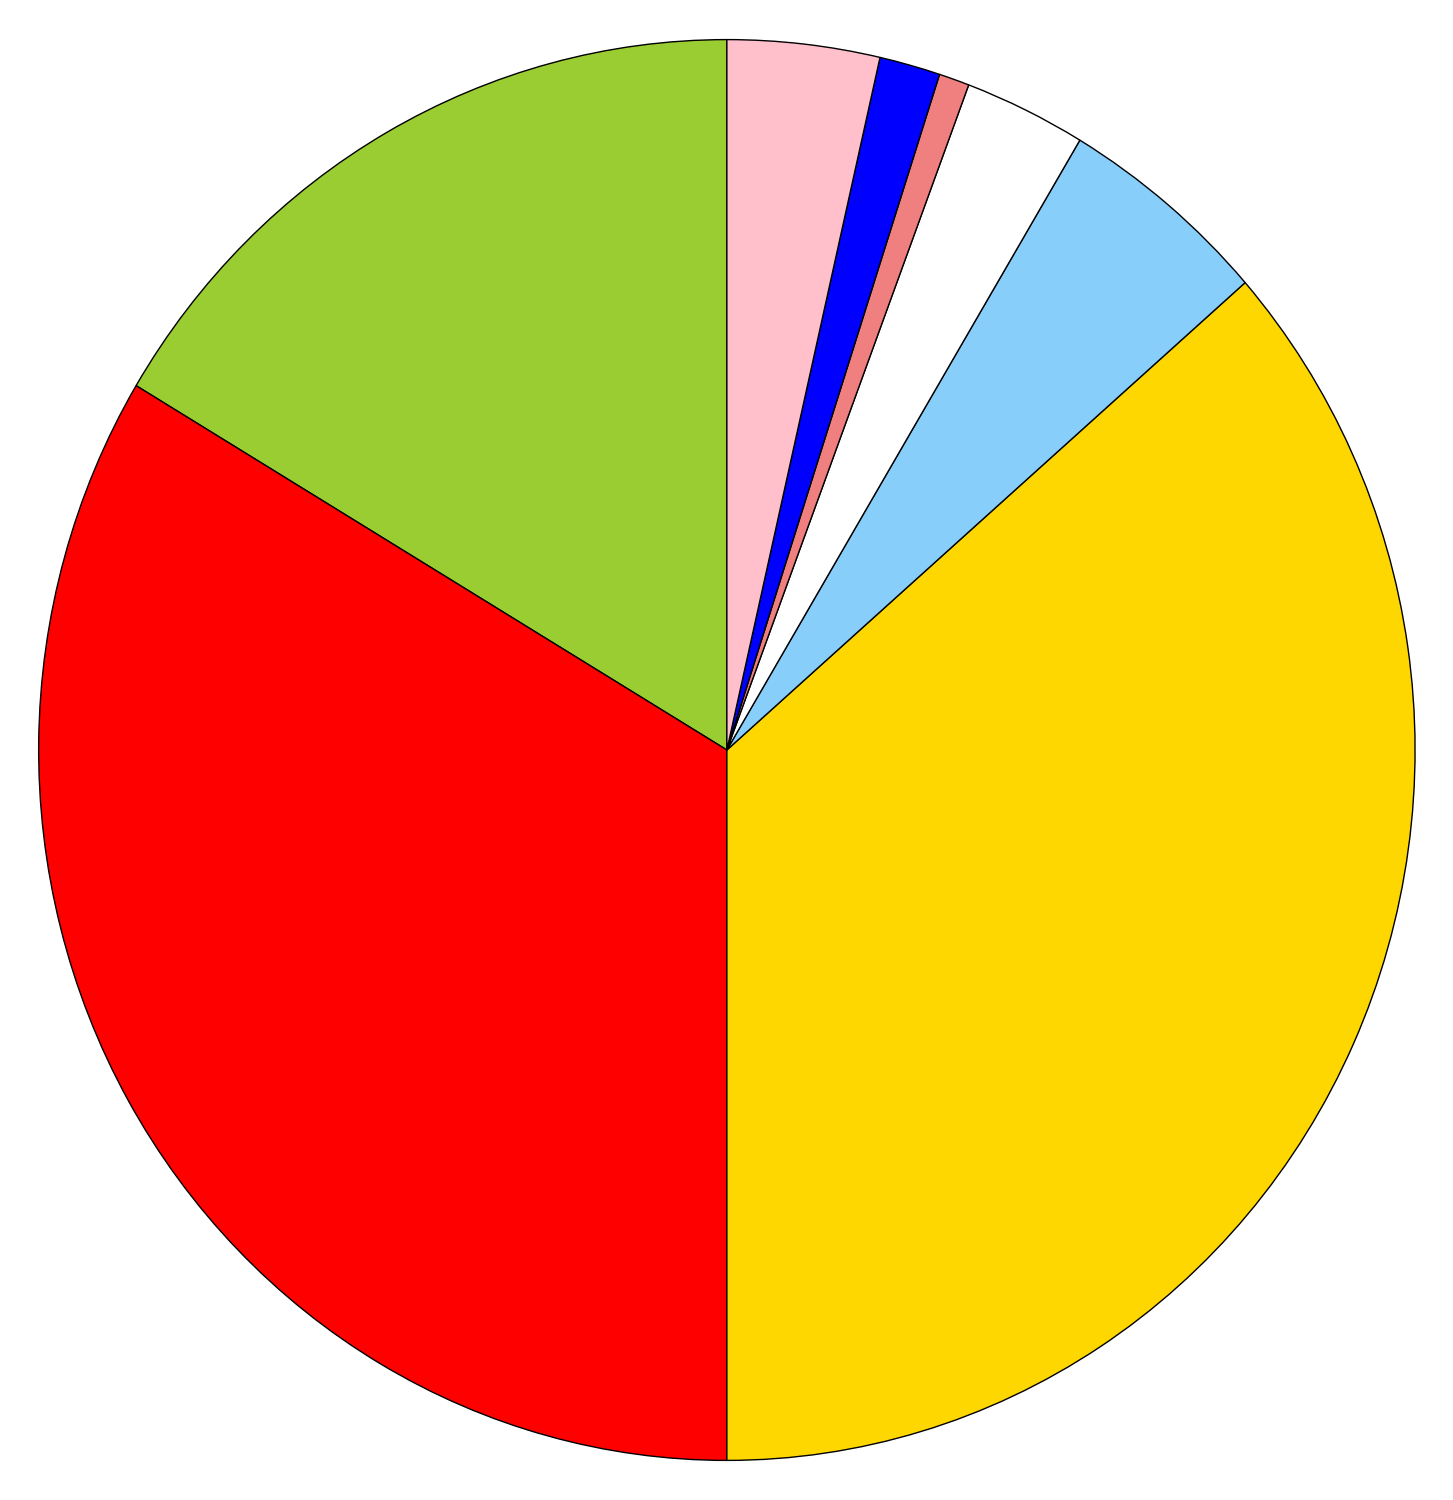
\includegraphics[width=\textwidth]{arousalALLSVM}
    \caption{SVM}
  \end{subfigure}
  
  \begin{subfigure}[b]{0.3\textwidth}
    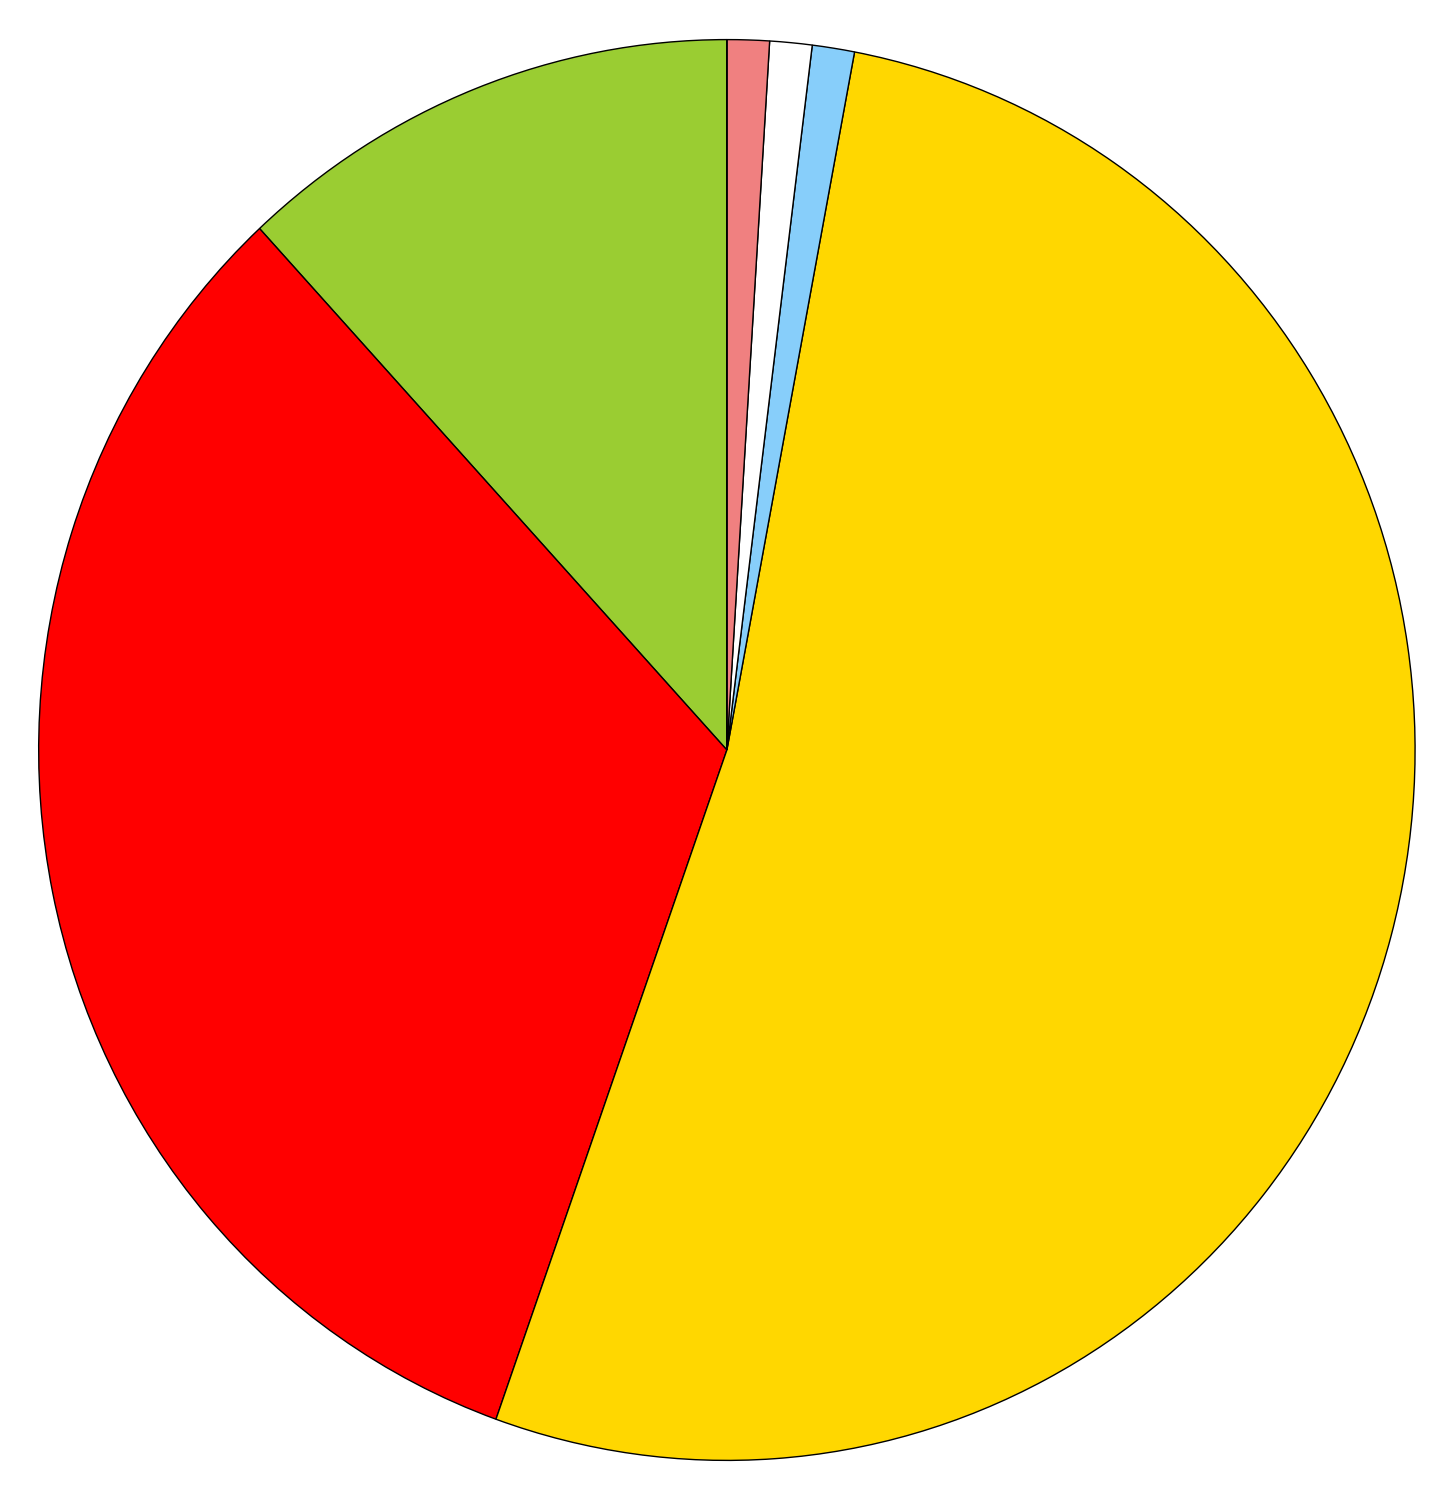
\includegraphics[width=\textwidth]{arousalALLLDA}
    \caption{LDA}
  \end{subfigure}
  \hfill
  \begin{subfigure}[b]{0.3\textwidth}
    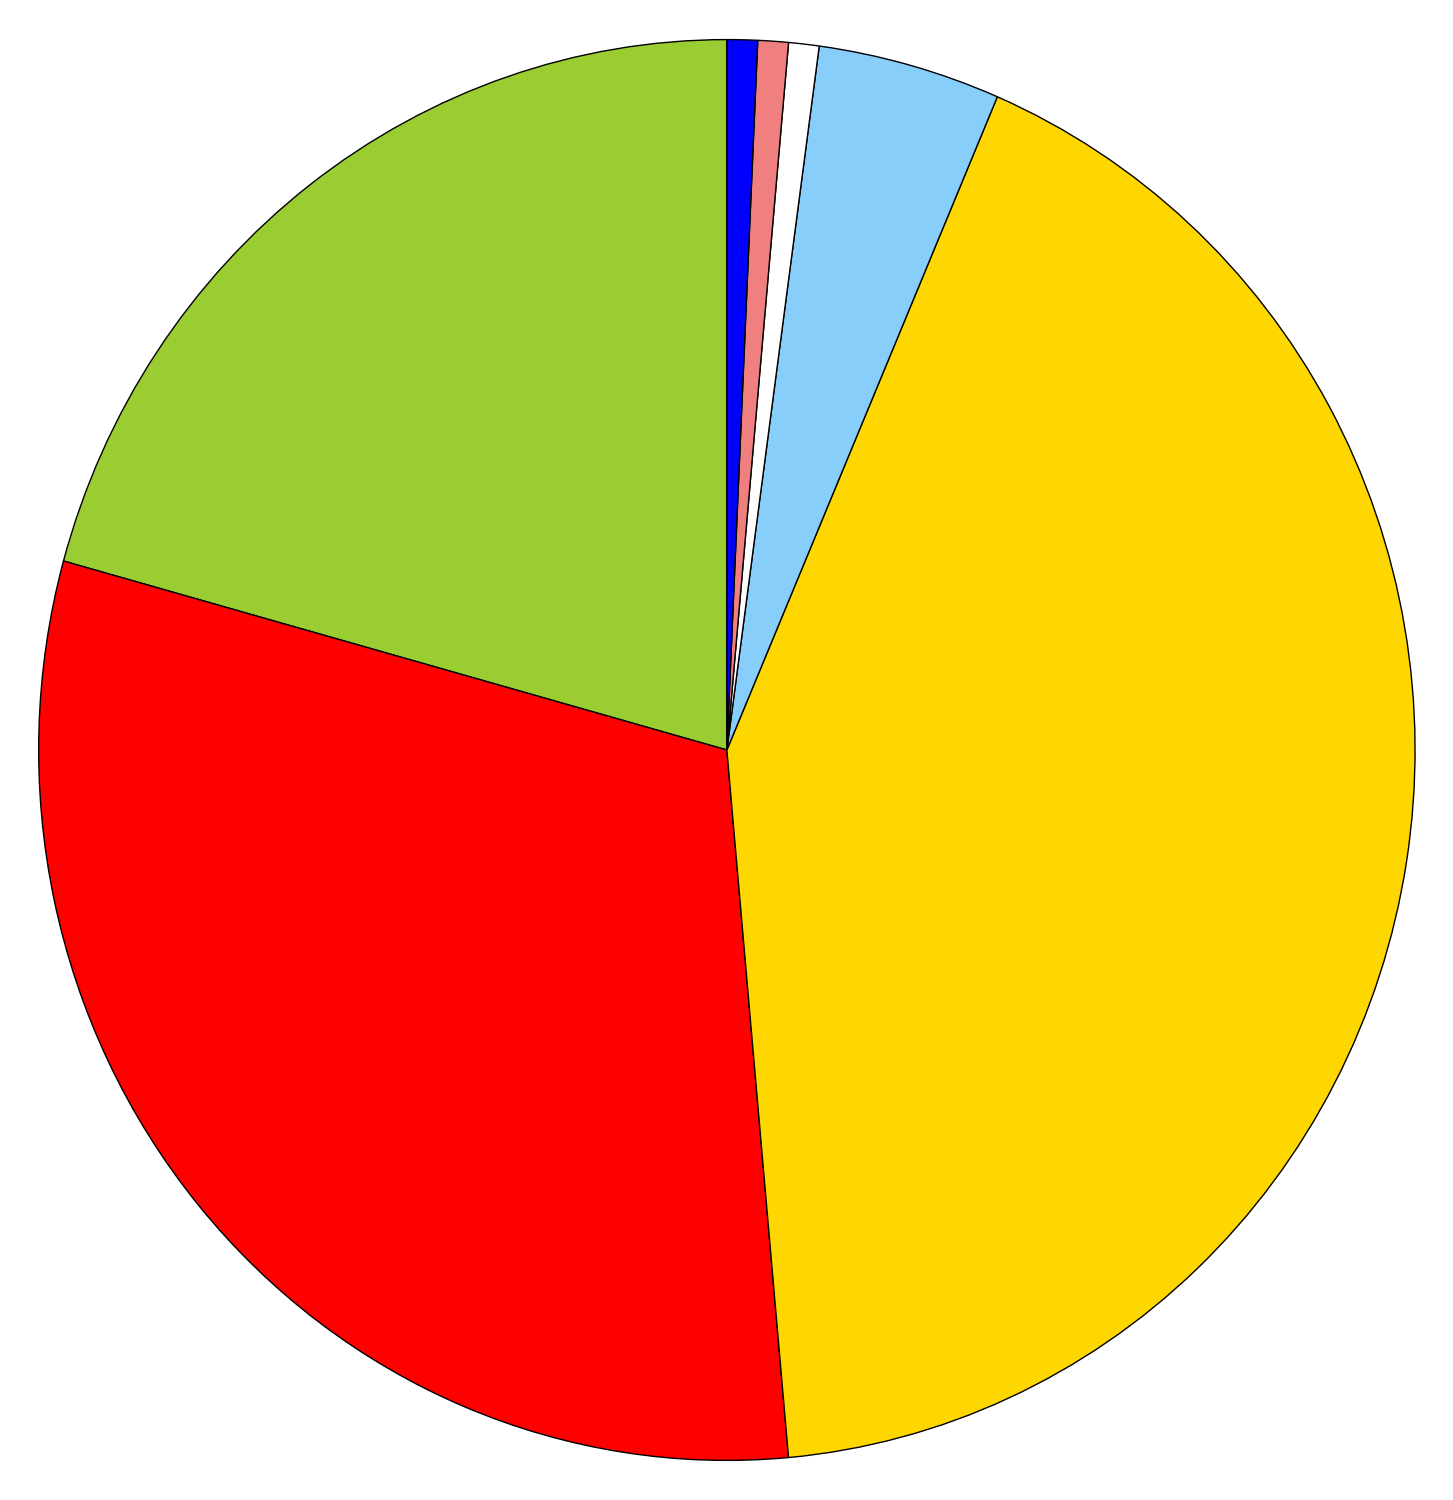
\includegraphics[width=\textwidth]{arousalALLL1}
    \caption{Lasso regression}
  \end{subfigure}
  \hfill
  \begin{subfigure}[b]{0.3\textwidth}
    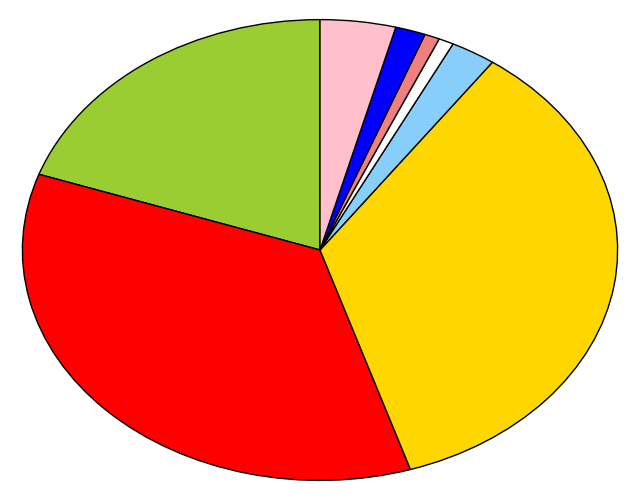
\includegraphics[width=\textwidth]{arousalALLL2}
    \caption{Ridge regression}
  \end{subfigure}
  
  \begin{subfigure}[b]{0.3\textwidth}
    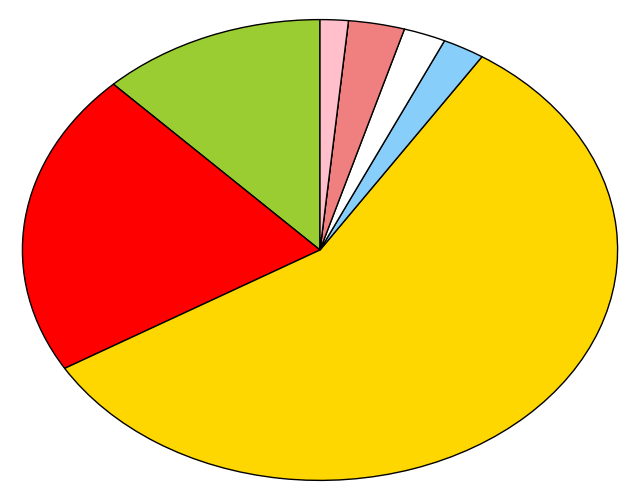
\includegraphics[width=\textwidth]{arousalALLRF}
    \caption{Random forests}
  \end{subfigure}
  \hfill
  \begin{subfigure}[b]{0.3\textwidth}
    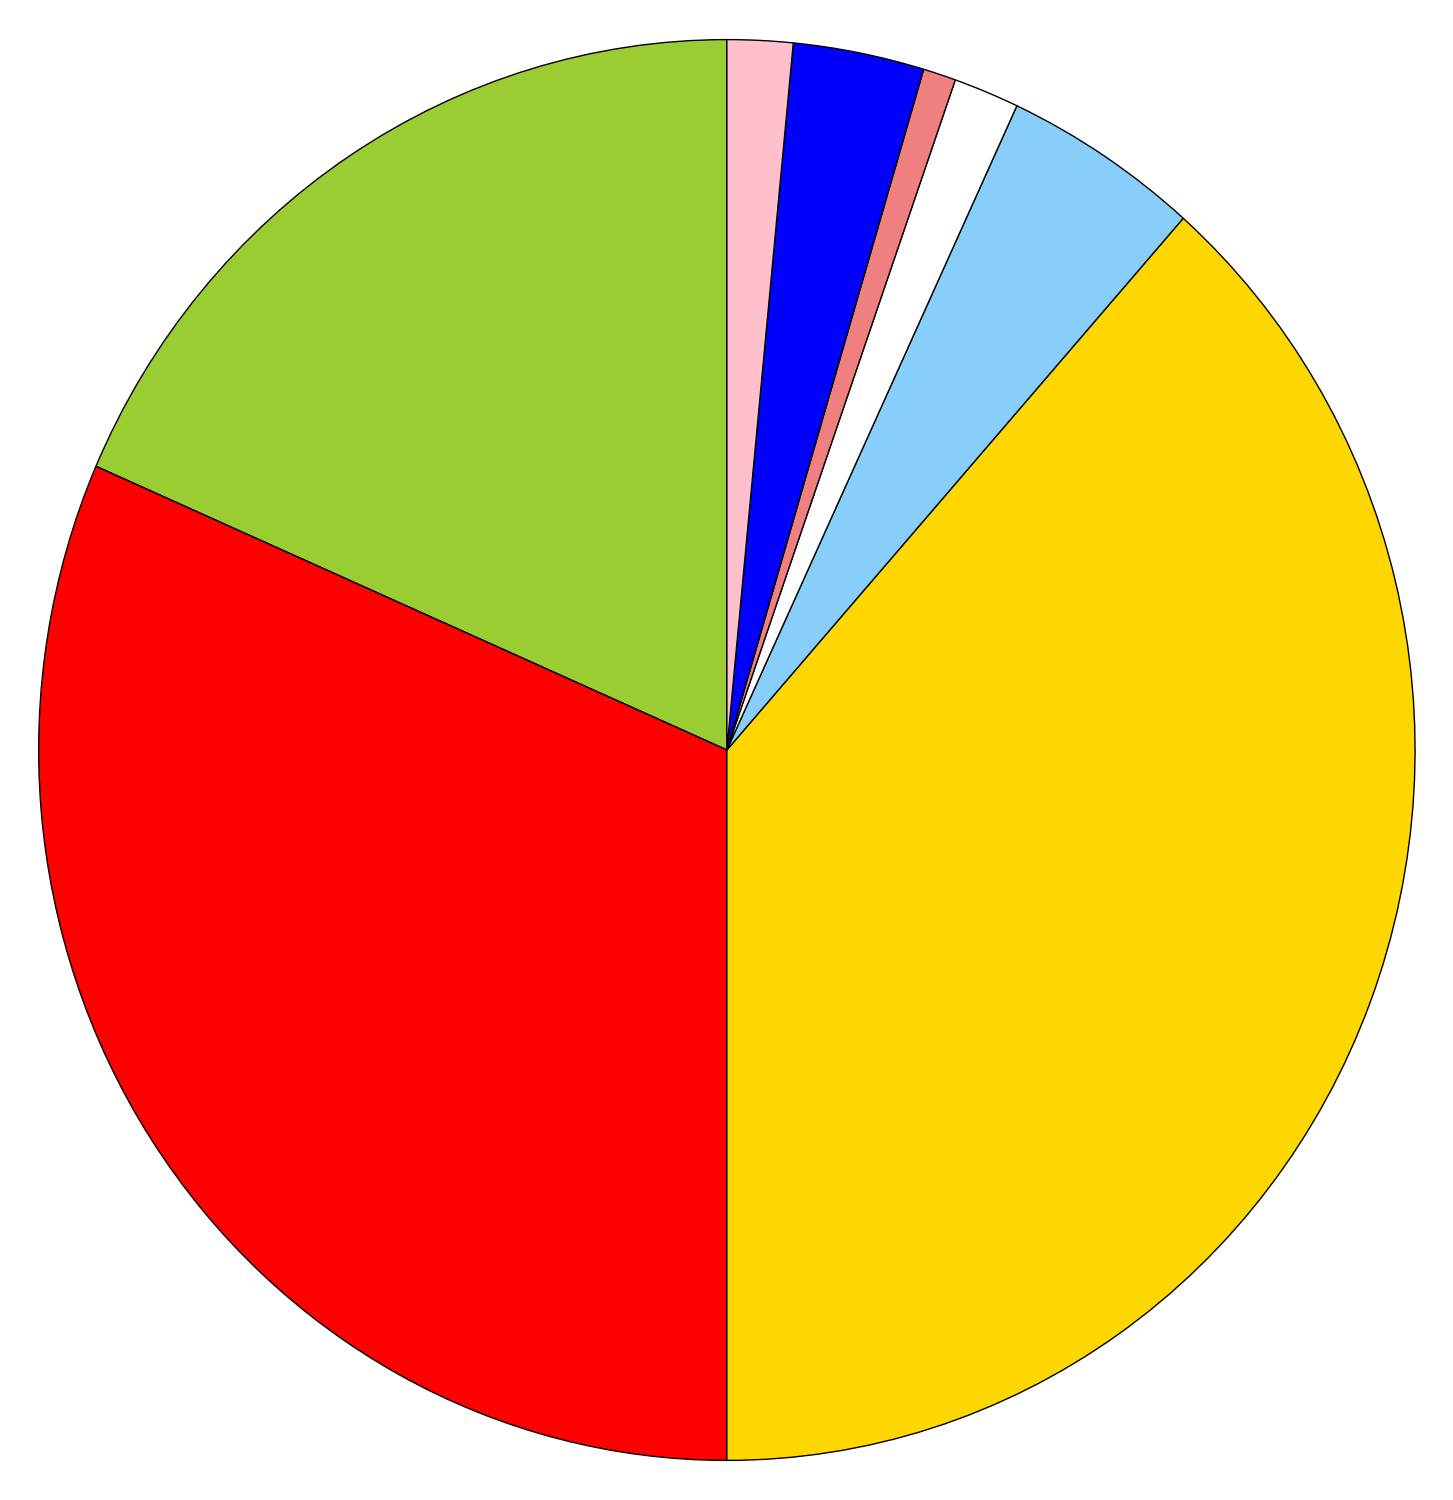
\includegraphics[width=\textwidth]{arousalALLPCA}
    \caption{PCA}
  \end{subfigure}
  \hfill
  \begin{subfigure}[b]{0.3\textwidth}
    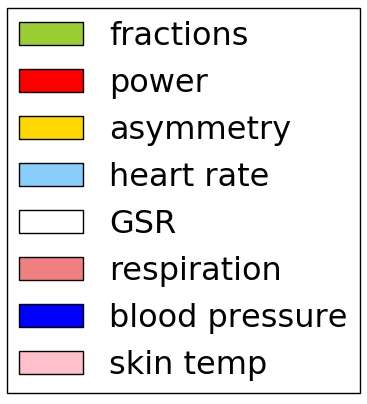
\includegraphics[width=\textwidth]{legend}
    \caption{Legend\label{arousalpieslegend}}
  \end{subfigure}
\caption{The distribution of the selected features for arousal classification of all persons combined of different feature selection methods. It is clear that the most valuable features are the asymmetry features combined with the power features. Furthermore, all feature selection methods agree that EEG features are dominant.\label{arousalpies}}
\end{figure}

\clearpage

\begin{figure}[!tbp]
  \centering
  \begin{subfigure}[b]{0.3\textwidth}
    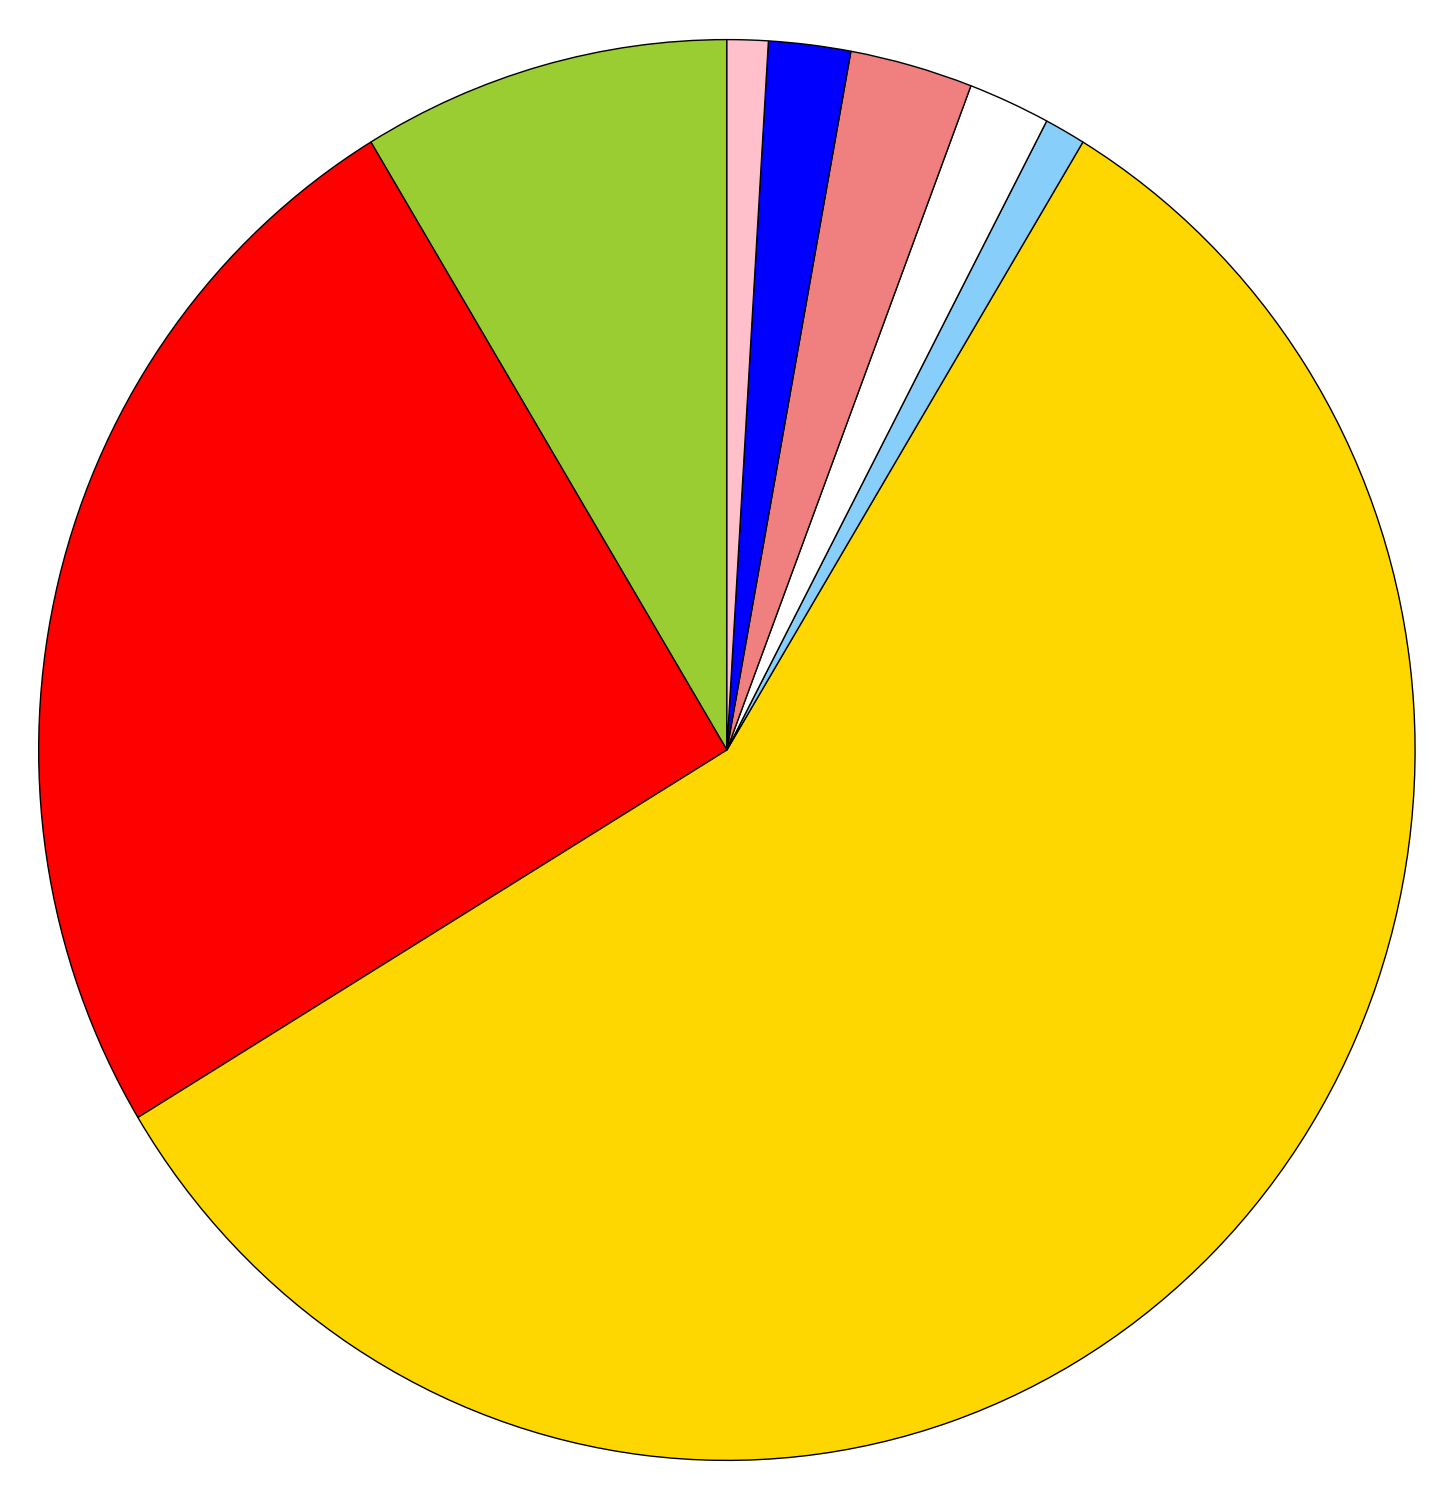
\includegraphics[width=\textwidth]{valenceALLpearsonR}
    \caption{Pearson correlation}
  \end{subfigure}
  \hfill
  \begin{subfigure}[b]{0.3\textwidth}
    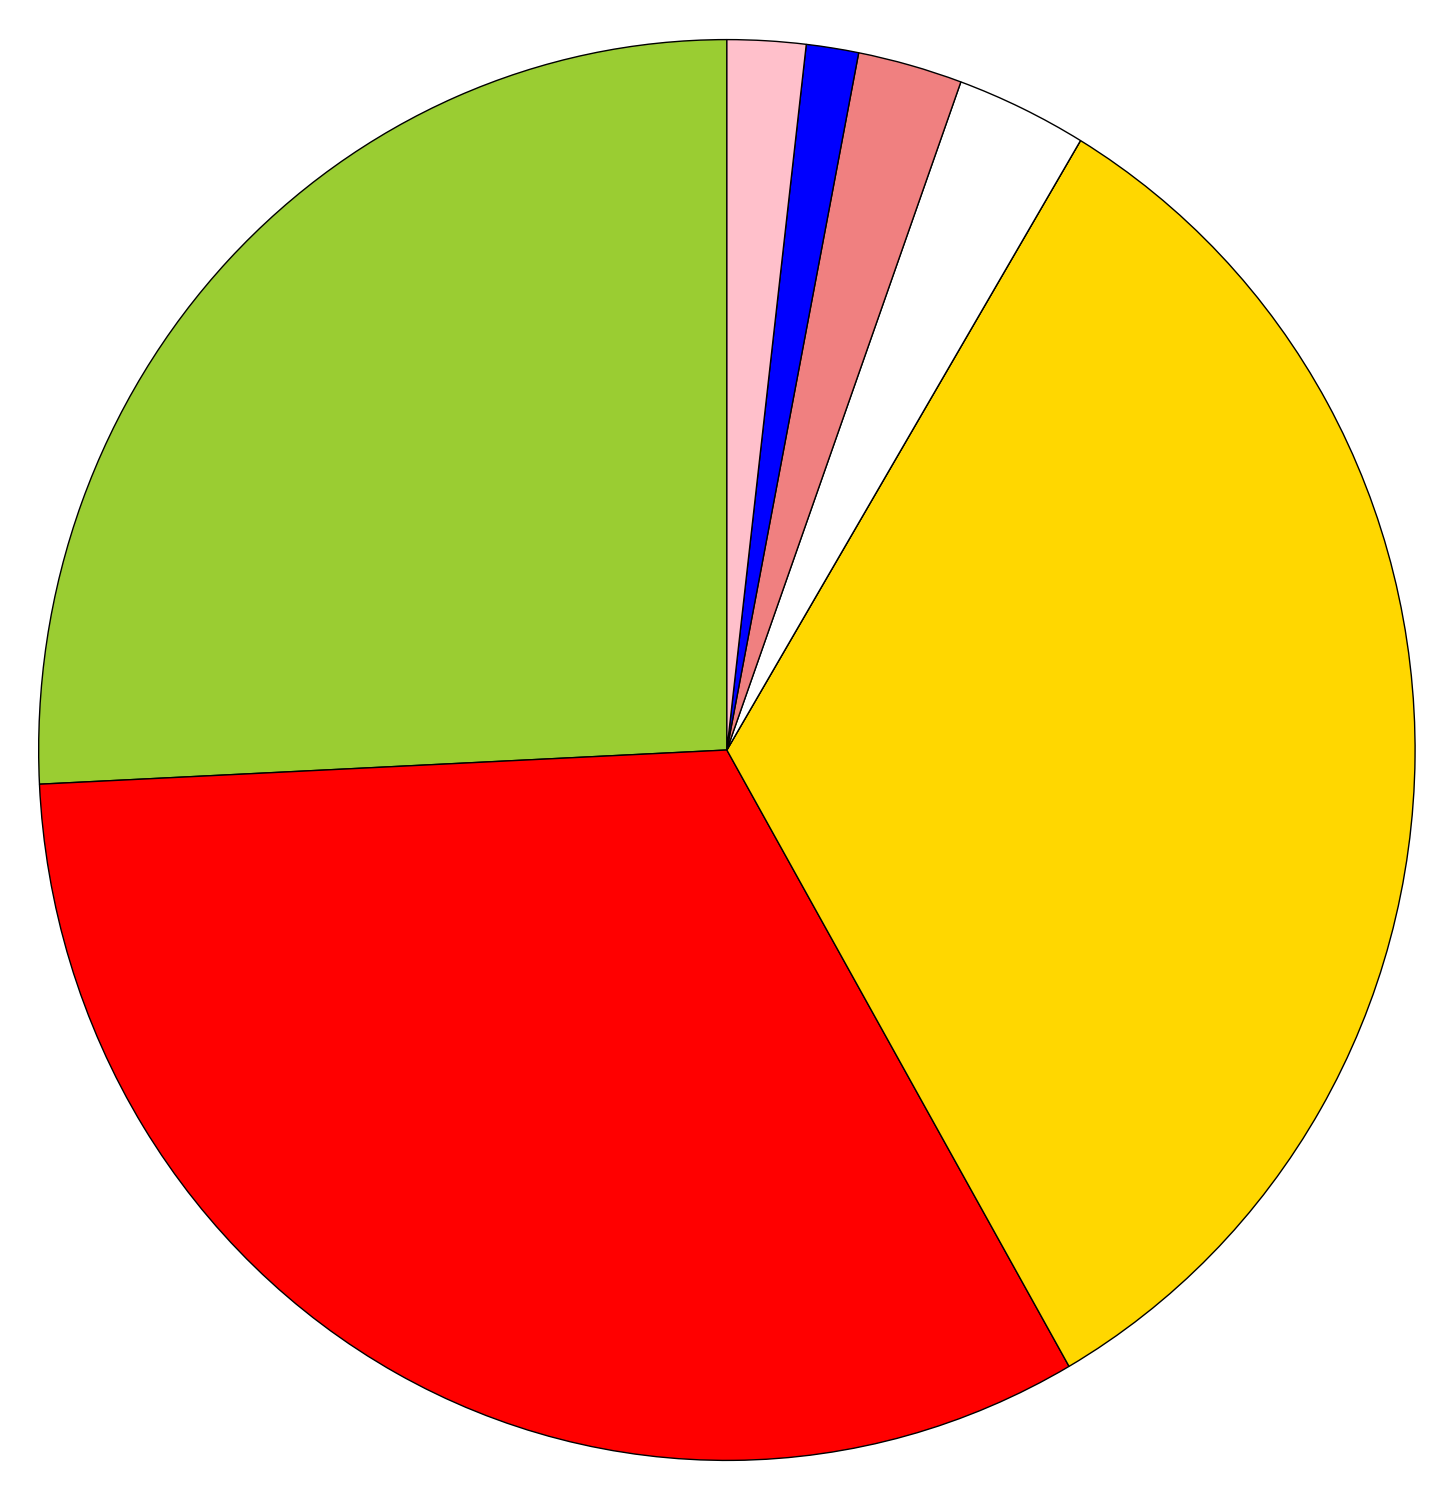
\includegraphics[width=\textwidth]{valenceALLMutInf}
    \caption{Mutual information}
  \end{subfigure}
  \hfill
  \begin{subfigure}[b]{0.3\textwidth}
    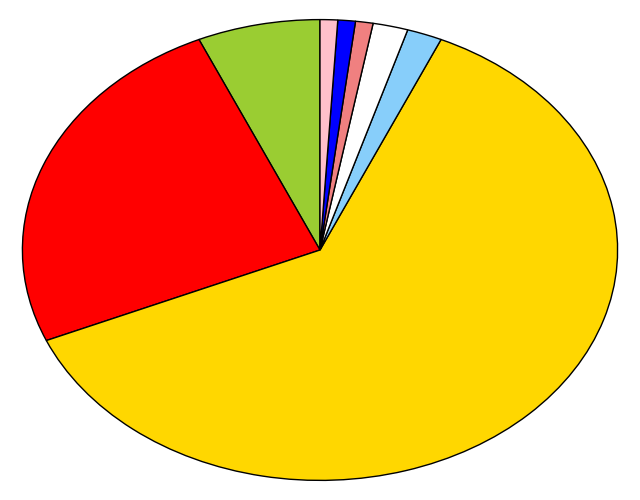
\includegraphics[width=\textwidth]{valenceALLdCorr}
    \caption{Distance Correlation}
  \end{subfigure}
  
  \begin{subfigure}[b]{0.3\textwidth}
    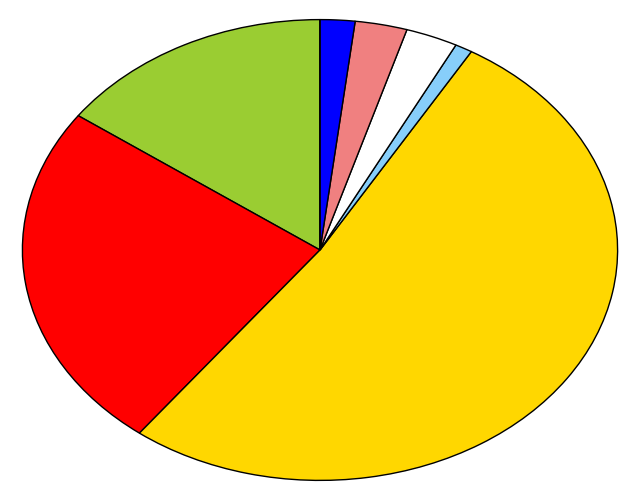
\includegraphics[width=\textwidth]{valenceALLANOVA}
    \caption{ANOVA}
  \end{subfigure}
  \hfill
  \begin{subfigure}[b]{0.3\textwidth}
    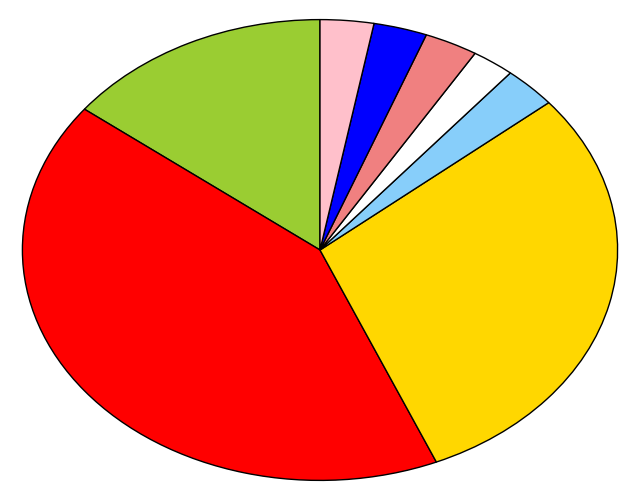
\includegraphics[width=\textwidth]{valenceALLLR}
    \caption{Linear regression}
  \end{subfigure}
  \hfill
  \begin{subfigure}[b]{0.3\textwidth}
    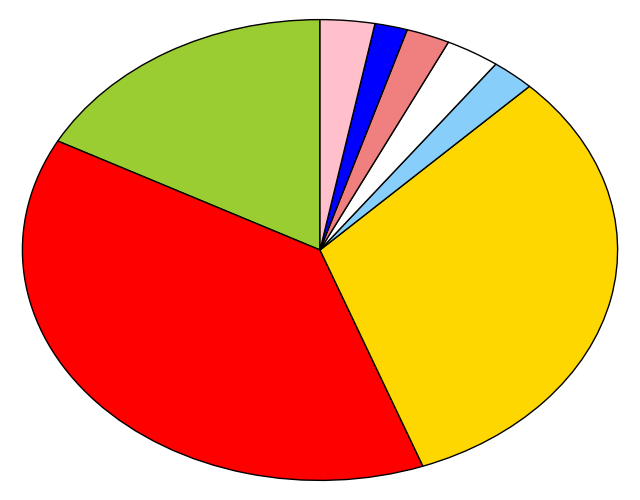
\includegraphics[width=\textwidth]{valenceALLSVM}
    \caption{SVM}
  \end{subfigure}
  
  \begin{subfigure}[b]{0.3\textwidth}
    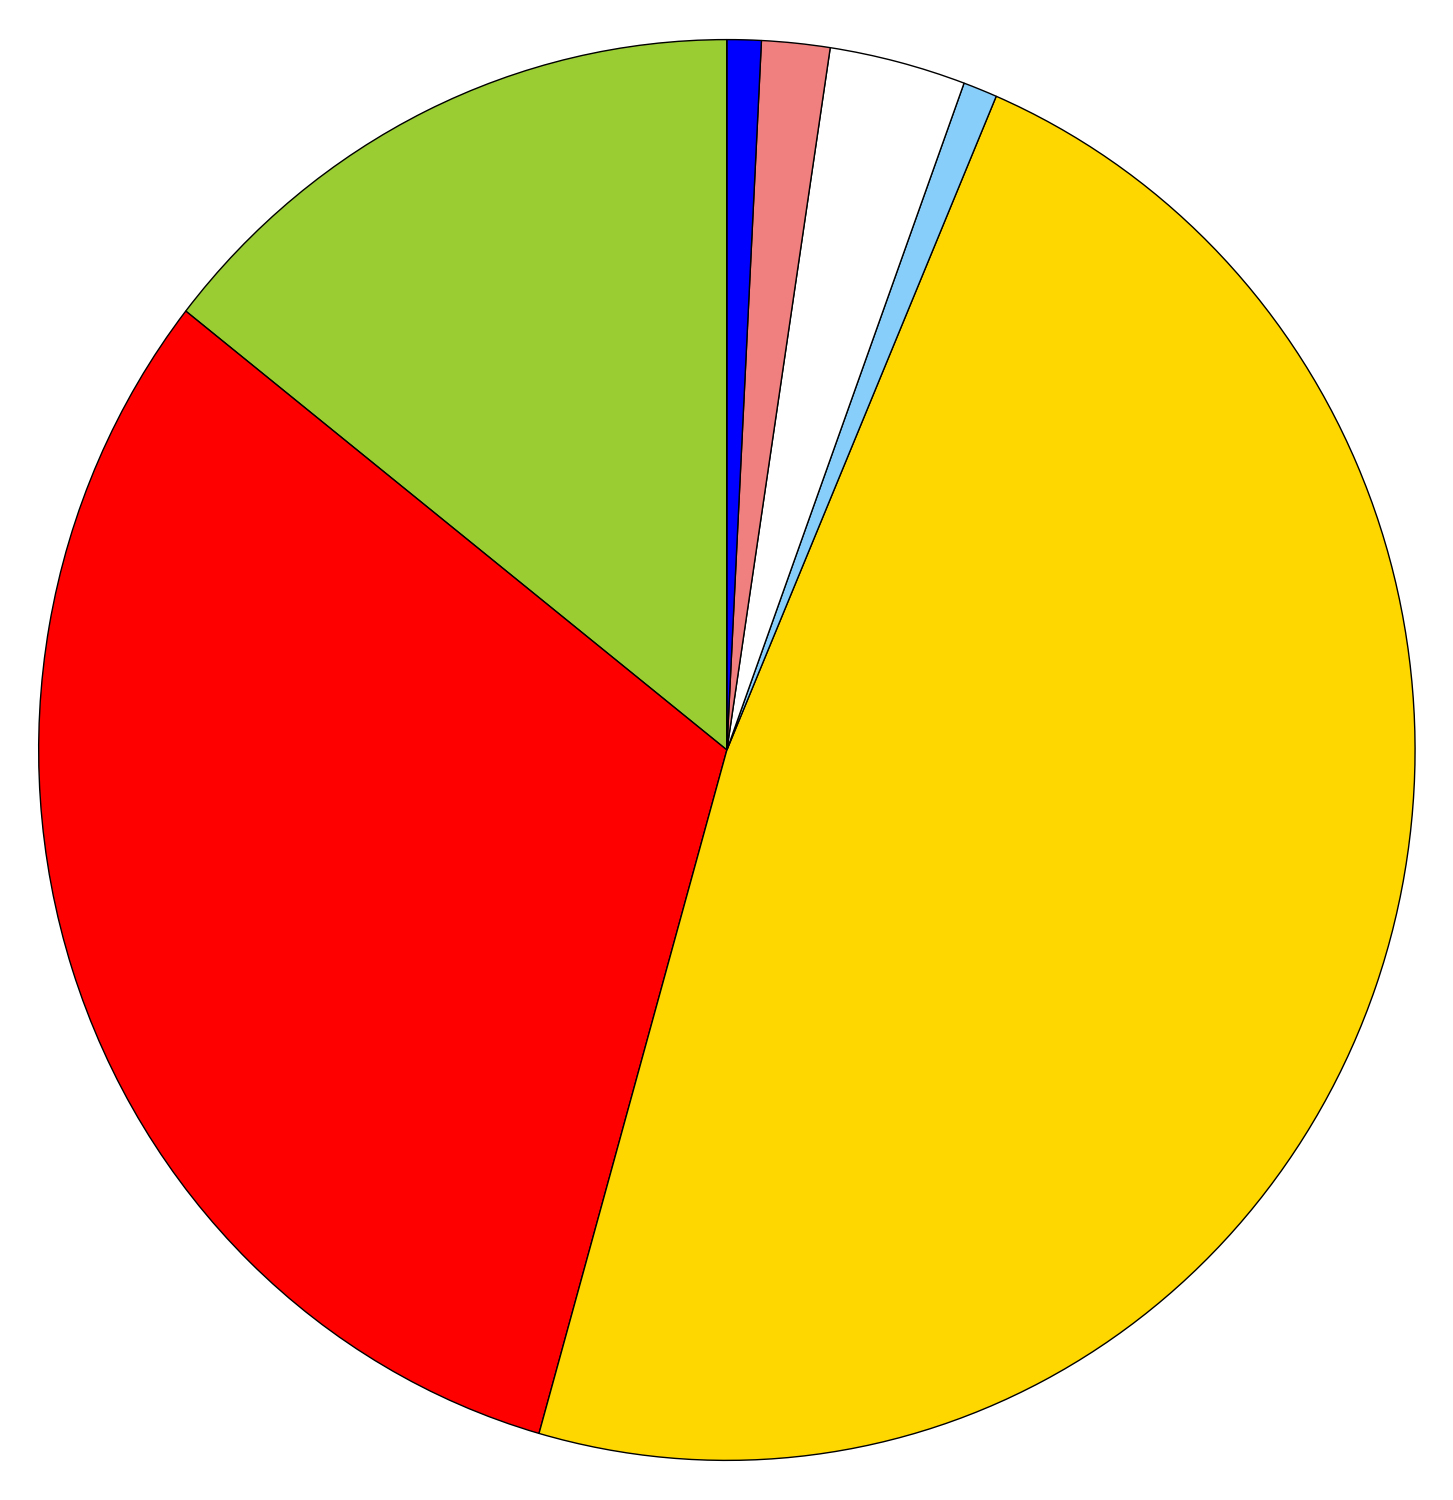
\includegraphics[width=\textwidth]{valenceALLLDA}
    \caption{LDA}
  \end{subfigure}
  \hfill
  \begin{subfigure}[b]{0.3\textwidth}
    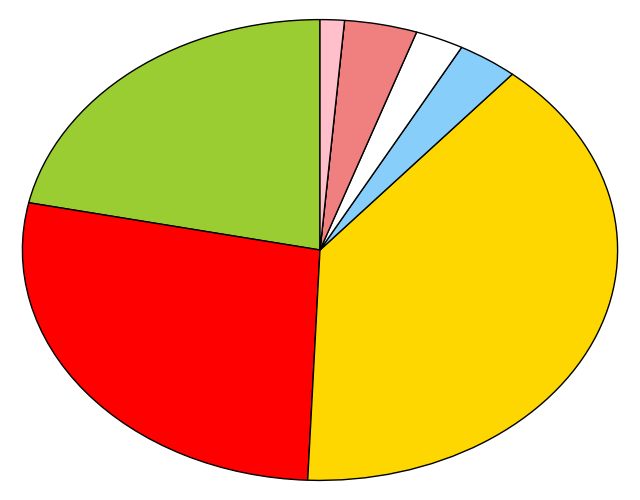
\includegraphics[width=\textwidth]{valenceALLL1}
    \caption{Lasso regression}
  \end{subfigure}
  \hfill
  \begin{subfigure}[b]{0.3\textwidth}
    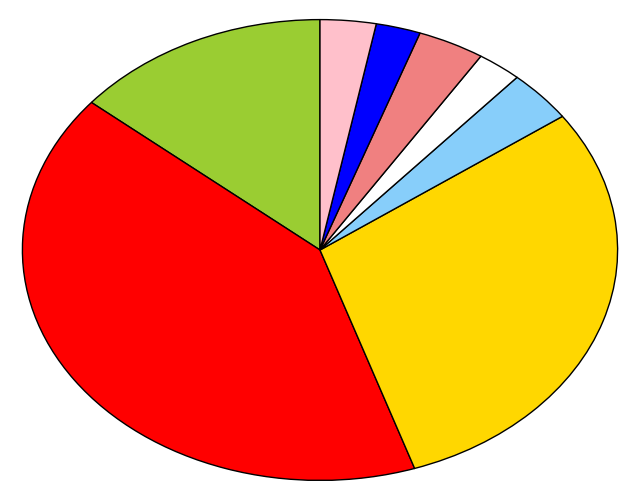
\includegraphics[width=\textwidth]{valenceALLL2}
    \caption{Ridge regression}
  \end{subfigure}
  
  \begin{subfigure}[b]{0.3\textwidth}
    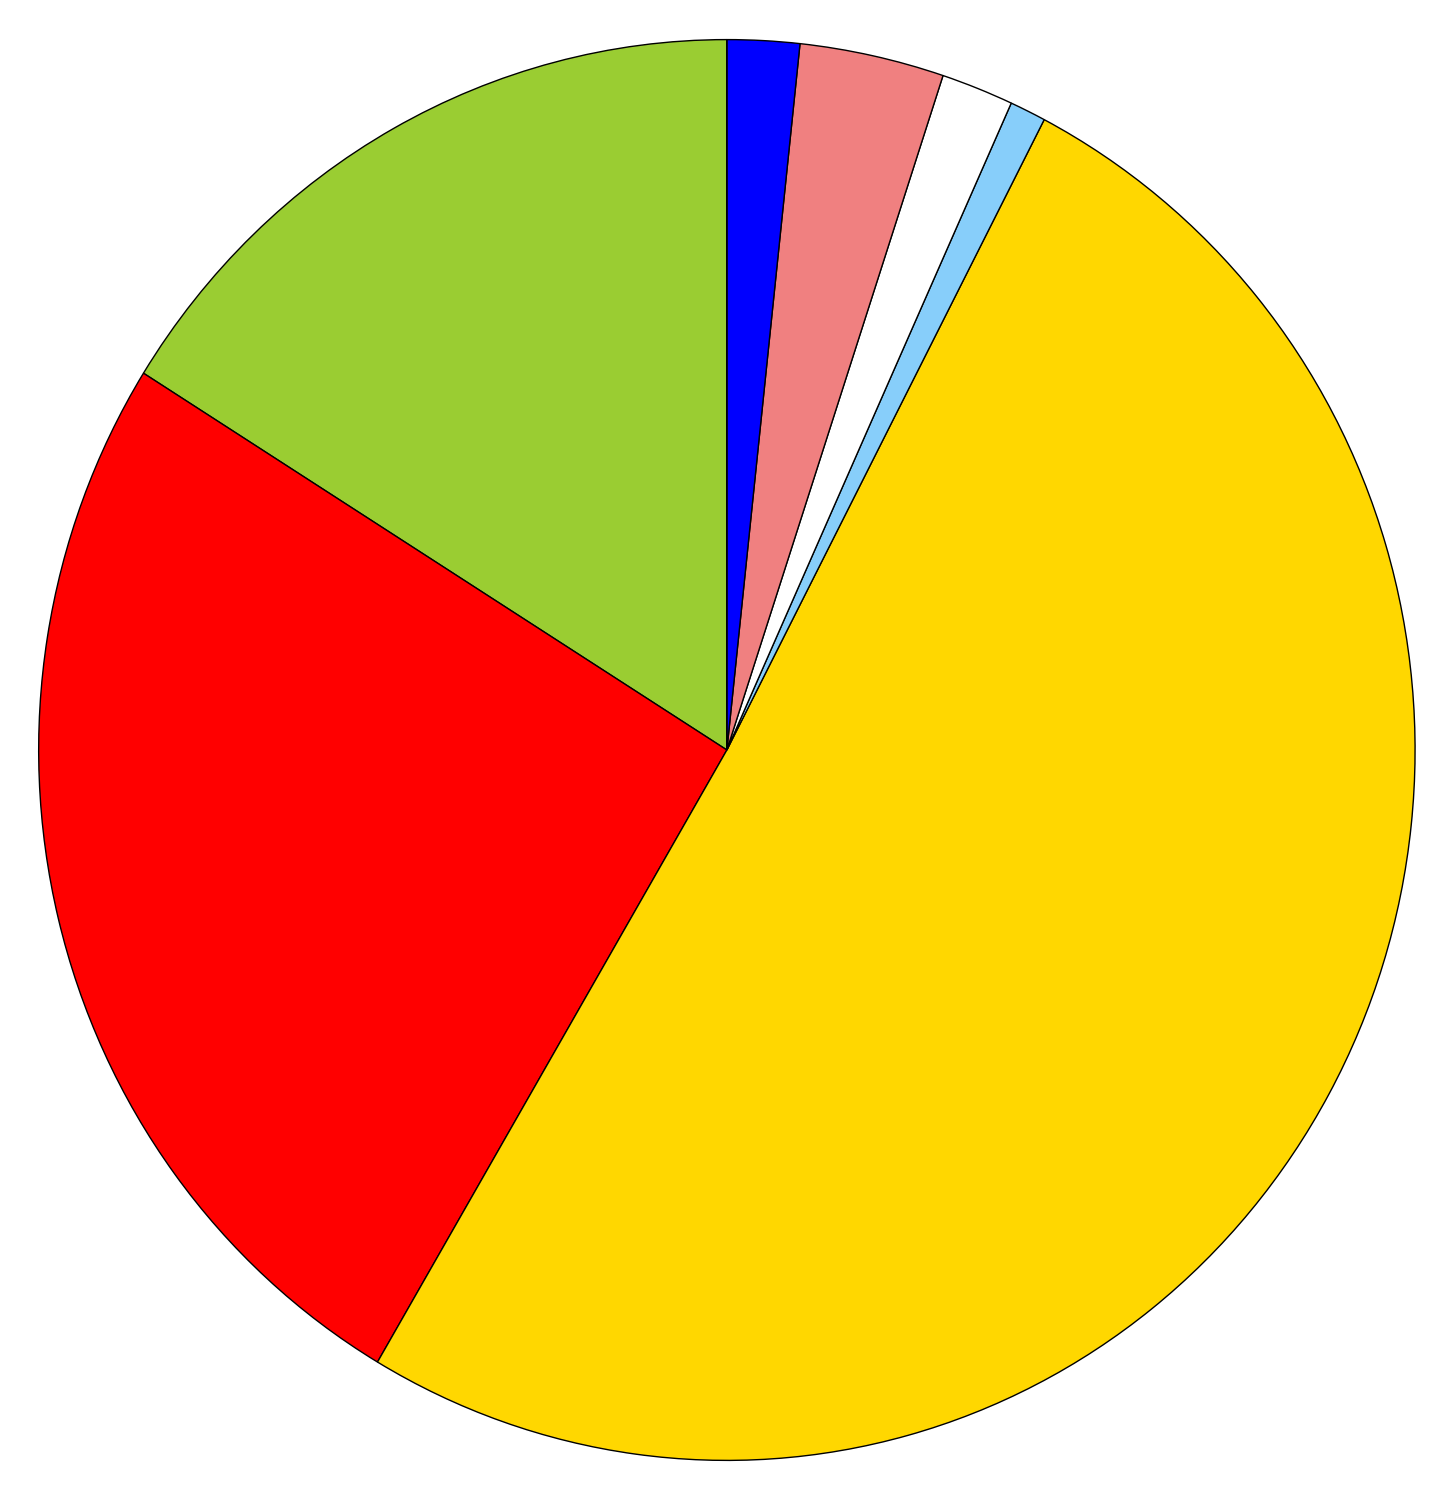
\includegraphics[width=\textwidth]{valenceALLRF}
    \caption{Random forests}
  \end{subfigure}
  \hfill
  \begin{subfigure}[b]{0.3\textwidth}
    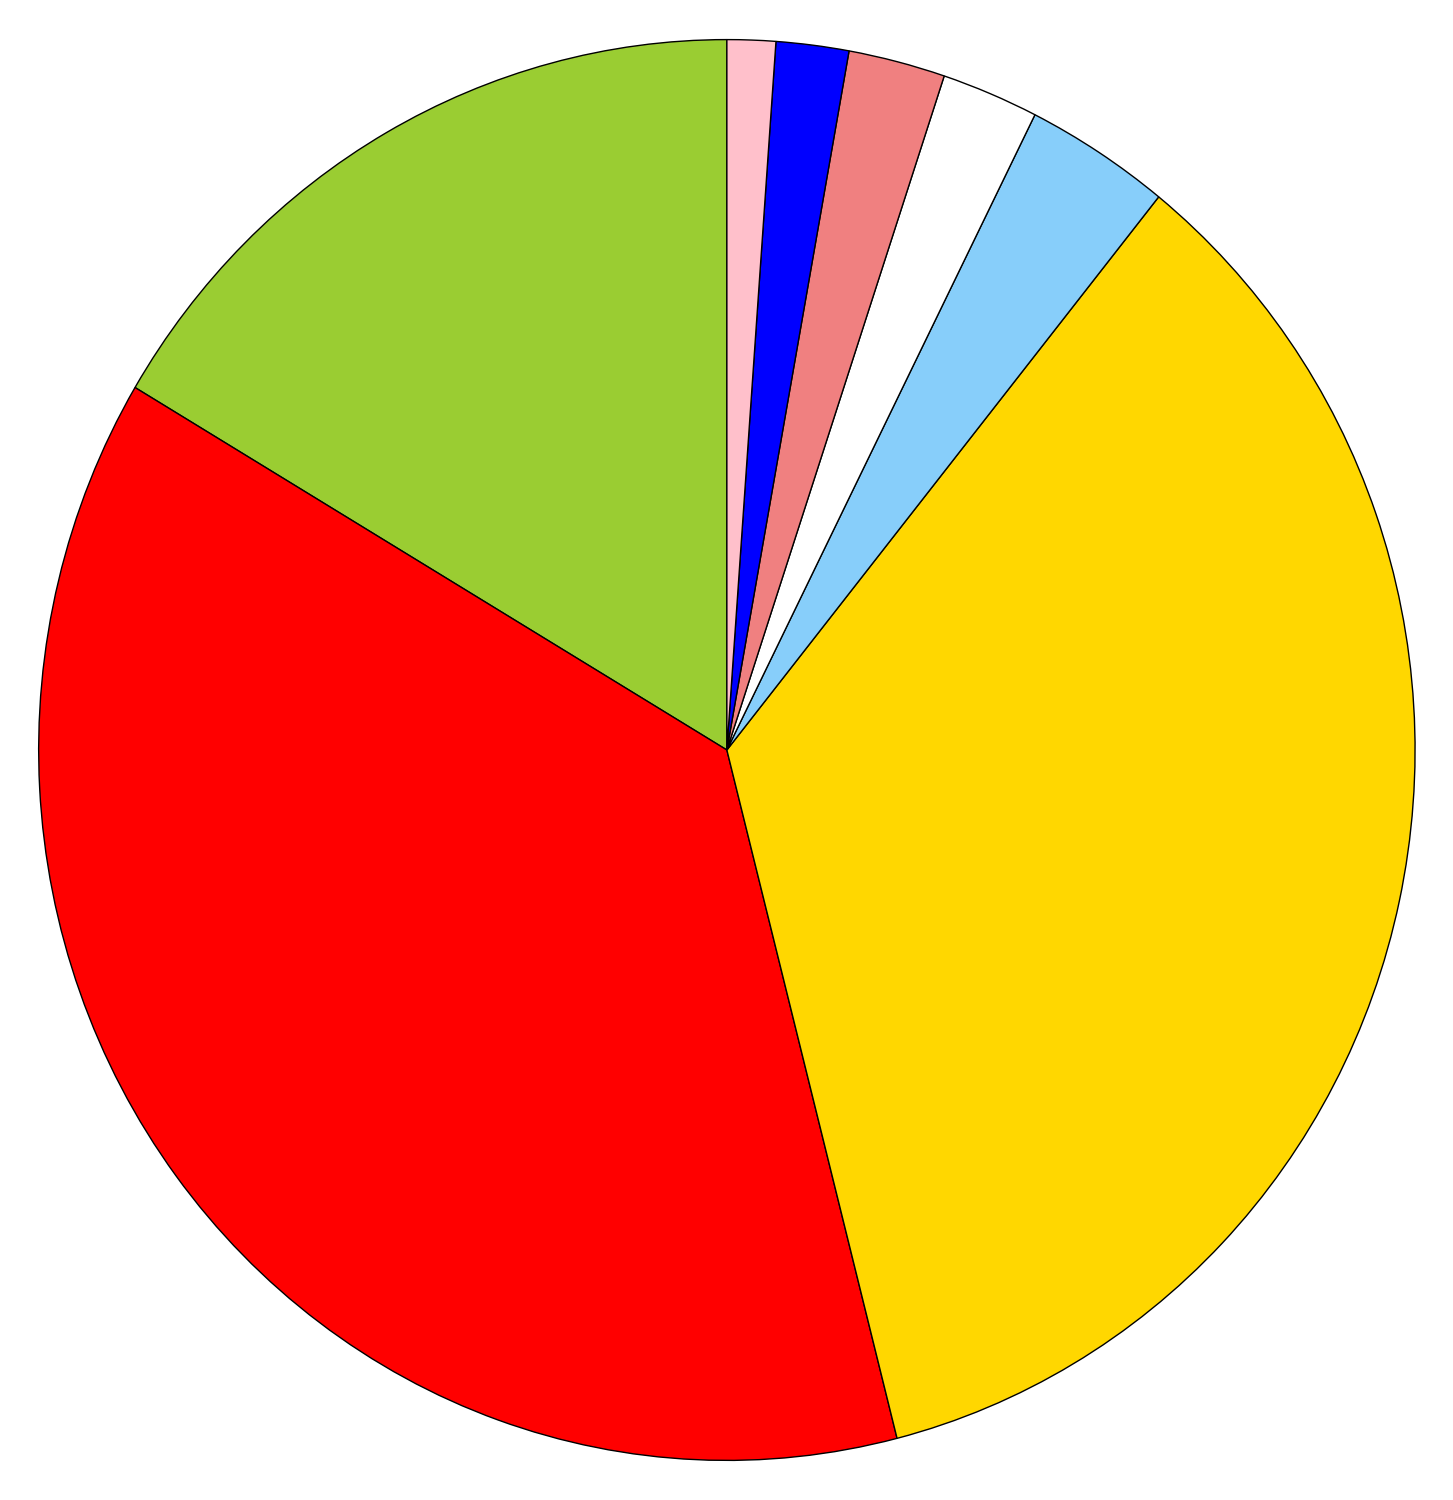
\includegraphics[width=\textwidth]{valenceALLPCA}
    \caption{PCA}
  \end{subfigure}
  \hfill
  \begin{subfigure}[b]{0.3\textwidth}
    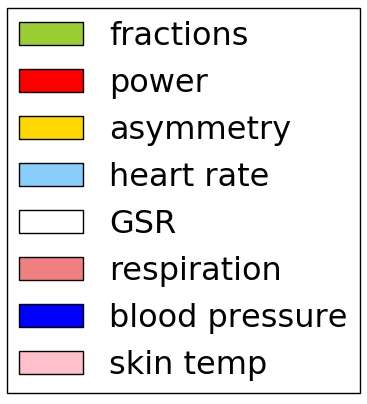
\includegraphics[width=\textwidth]{legend}
    \caption{Legend\label{valencepieslegend}}
  \end{subfigure}
\caption{The distribution of the selected features for valence classification of all persons combined of different feature selection methods. It is clear that the most valuable features are the asymmetry features combined with the power features. Furthermore, all feature selection methods agree that EEG features are dominant.\label{valencepies}}
\end{figure}
\clearpage

The fact that non-EEG features are almost never chosen might indicate that they are less important. In an attempt to further investigate the difference between EEG features and non-EEG features, the performance of three different feature sets was compared. The first feature set is the previously used feature set with all possible features. The second and third feature sets contained only EEG and non-EEG features respectively. The feature selection was done with random forest, as this method had the best average performance and is the most advanced. 

\npar

The resulting performances of these different features sets are displayed in Figure \ref{arousalphyeegall} for arousal and in Figure \ref{valencephyeegall} for valence. The exact values are shown in Table \ref{phyeegalltable}.

\mijnfiguur{width=1.\textwidth}{arousalphyeegall}{The average and standard deviation of the test accuracies of arousal classification for all, EEG and non-EEG features, see also Table \ref{phyeegalltable}}

\mijnfiguur{width=1.\textwidth}{valencephyeegall}{The average and standard deviation of the test accuracies of valence classification for all, EEG and non-EEG features, see also Table \ref{phyeegalltable}}

\begin{table}[H]
\centering
\caption{The average and standard deviation of the test accuracies (over the different persons) for the different feature sets, using the random forest feature selection model.\label{phyeegalltable}}
\begin{tabular}{l|ll|ll}
         & \textbf{Arousal} &         & \textbf{Valence} &         \\
\textbf{Feat set} & \textbf{avg acc} & \textbf{std acc} & \textbf{avg acc} & \textbf{std acc} \\ \hline 
\textbf{all}      & 0.7000  & 0.1369  & 0.7375  & 0.1293  \\
\textbf{EEG}      & 0.7188  & 0.1310  & 0.7281  & 0.1179  \\
\textbf{non-EEG}  & 0.6031  & 0.1425  & 0.6031  & 0.1591 
\end{tabular}
\end{table}

It is clear that for both valence and arousal, the average test performances are lower in case only non-EEG features are used. This is confirmed by the p-values in Table \ref{pvals} below:

\begin{table}[H]
\centering
\caption{P-values for the comparison of the performance of different feature sets.\label{pvals}}
\begin{tabular}{l|lll}
	    		 & \textbf{all / EEG} & \textbf{all / non-EEG} & \textbf{EEG / non-EEG} \\ \hline
\textbf{Arousal} & $0.4386$          & $5.891 * 10^{-7}$  & $1.201 * 10^{-4}$ \\
\textbf{Valence} & $0.6817$          & $1.993 * 10^{-9}$  & $1.763 * 10^{-6}$                 
\end{tabular}
\end{table}
\clearpage

Next, for each of the three feature sets, a comparison of the selected features was made. As you can see on Figure \ref{arousalEEGpies} for arousal and Figure \ref{valenceEEGpies}, displayed on the following pages, the features are again mostly asymmetry features, followed by the power features. The fraction category gives only limited insight for both valence and arousal. The EEG and ALL set have similar performances, which was expected as they both use very similar features.

\npar

The results for the non-EEG features are shown in Figure \ref{arousalnon-EEGpies} for arousal and Figure \ref{valencenon-EEGpies} for valence, on the following pages.
Here, no single category can be labelled as most important. This is the case for both arousal and valence. However, the feature that was selected the most as being the most important for one person was the GSR, which measures perspiration. In case of valence, the first selected features were heart rate and GSR.

\clearpage
\begin{figure}[!tbp]
  \centering
  \begin{subfigure}[b]{0.3\textwidth}
    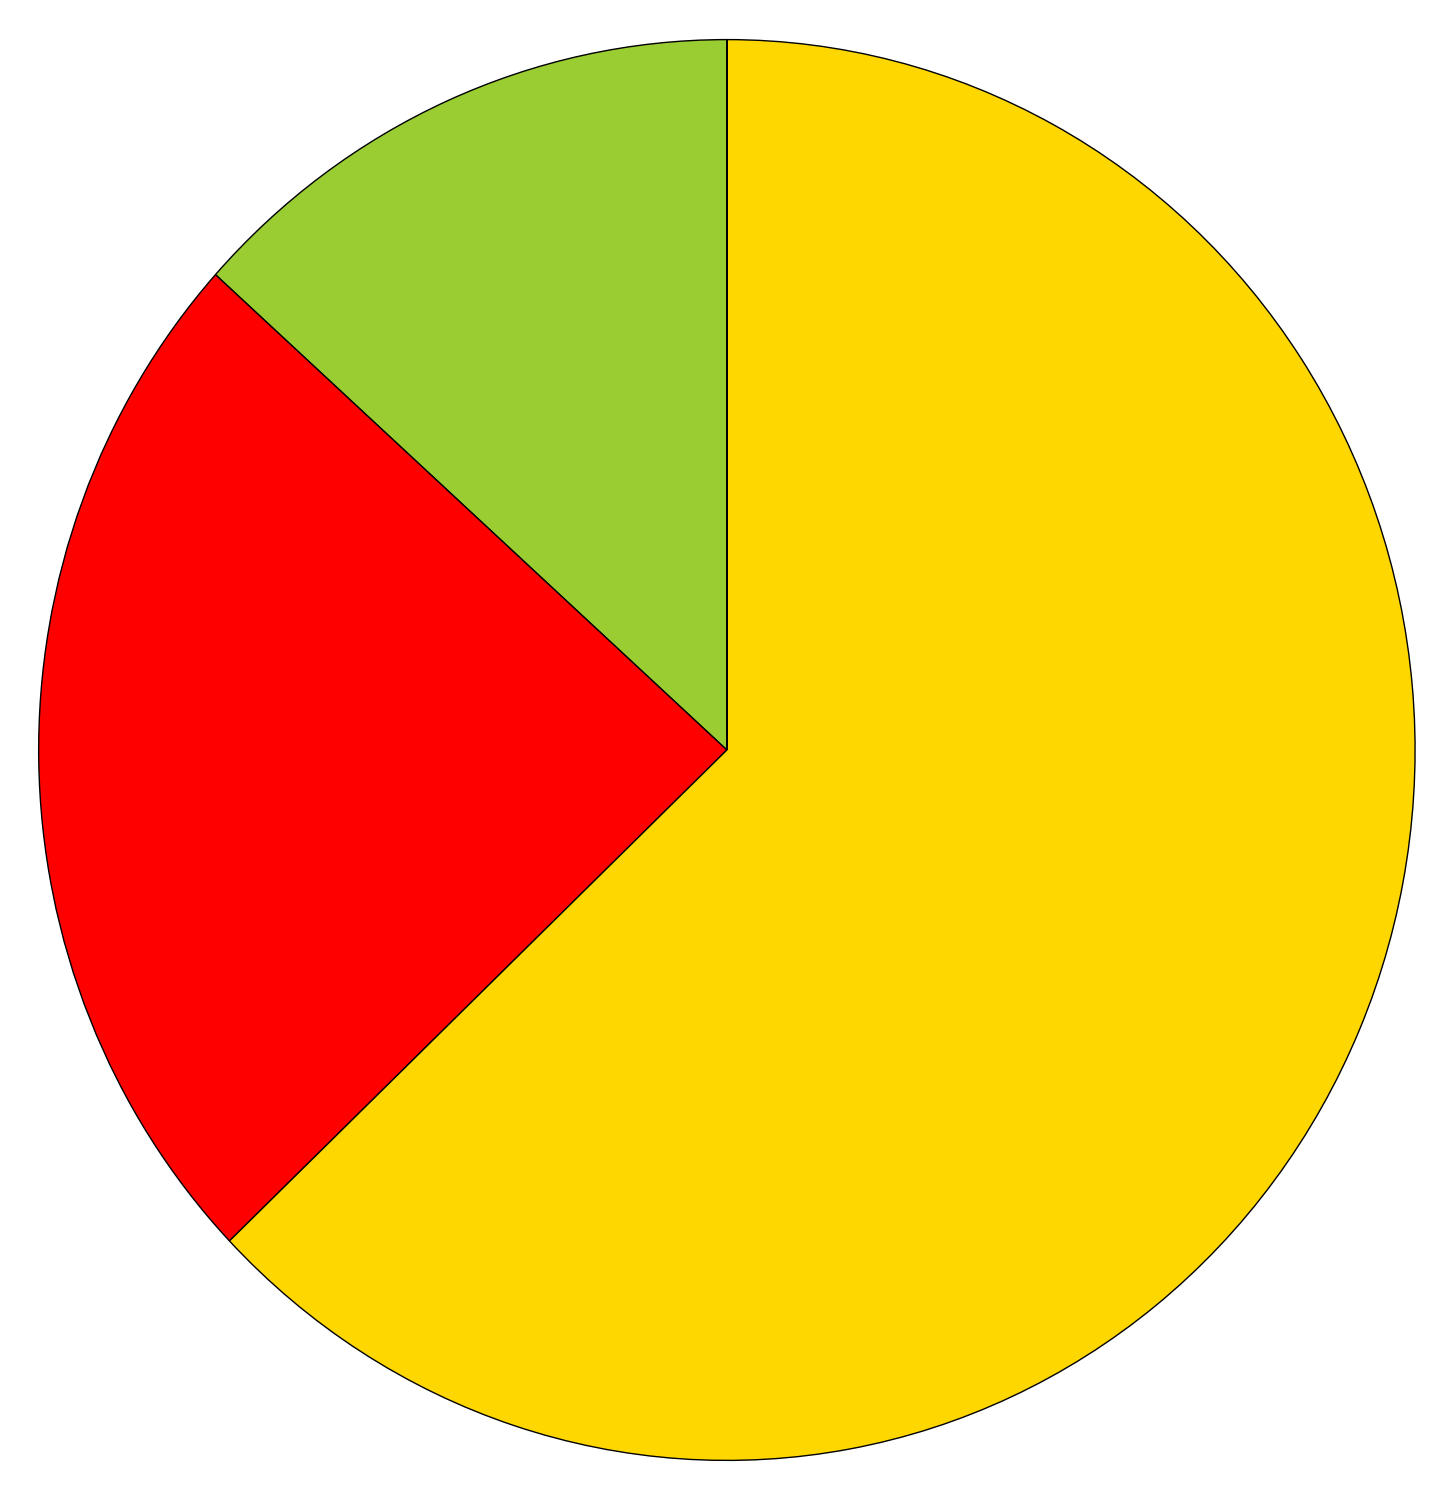
\includegraphics[width=\textwidth]{arousalEEGpearsonR}
    \caption{Pearson correlation}
  \end{subfigure}
  \hfill
  \begin{subfigure}[b]{0.3\textwidth}
    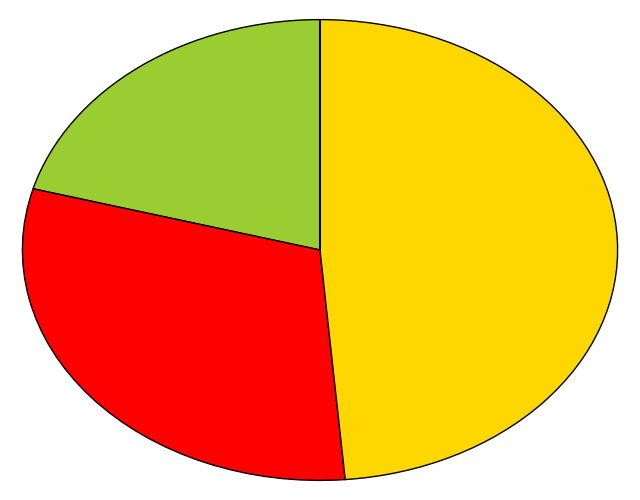
\includegraphics[width=\textwidth]{arousalEEGMutInf}
    \caption{Mutual information}
  \end{subfigure}
  \hfill
  \begin{subfigure}[b]{0.3\textwidth}
    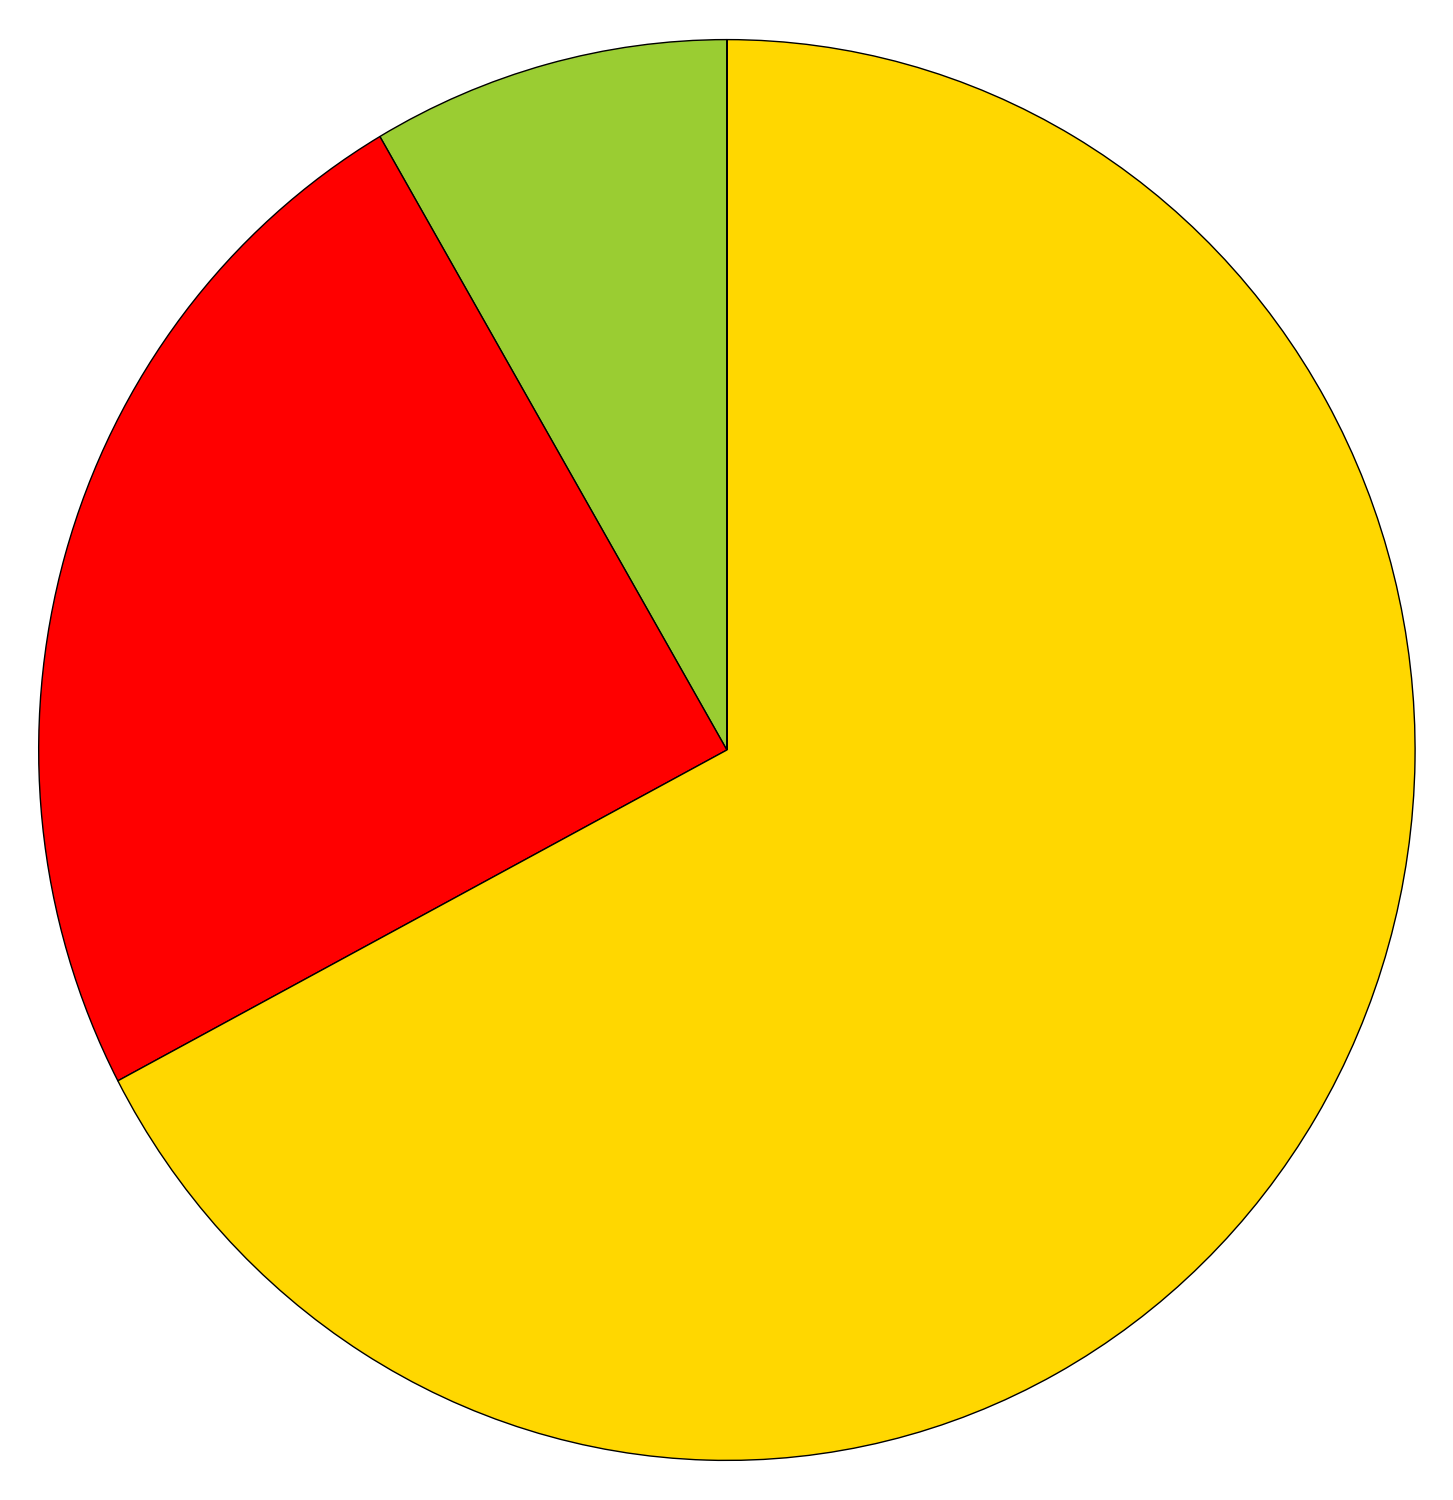
\includegraphics[width=\textwidth]{arousalEEGdCorr}
    \caption{Distance Correlation}
  \end{subfigure}
  
  \begin{subfigure}[b]{0.3\textwidth}
    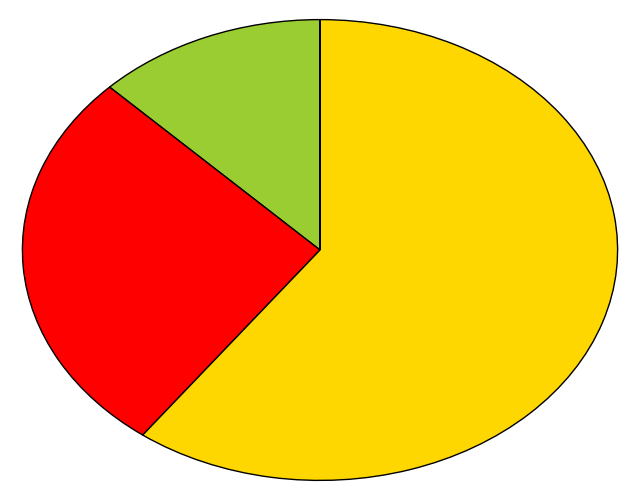
\includegraphics[width=\textwidth]{arousalEEGANOVA}
    \caption{ANOVA}
  \end{subfigure}
  \hfill
  \begin{subfigure}[b]{0.3\textwidth}
    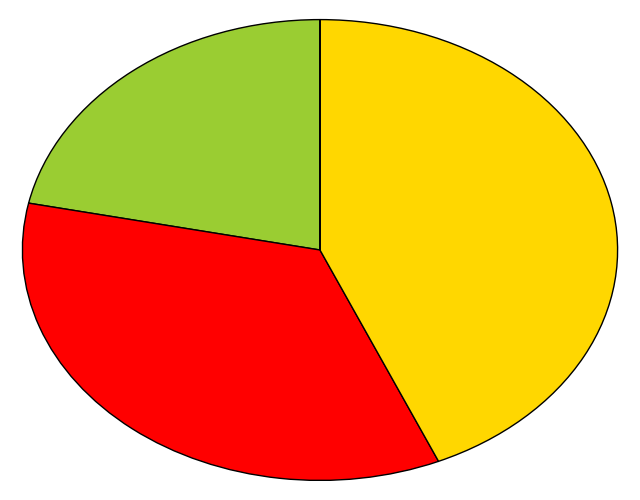
\includegraphics[width=\textwidth]{arousalEEGLR}
    \caption{Linear regression}
  \end{subfigure}
  \hfill
  \begin{subfigure}[b]{0.3\textwidth}
    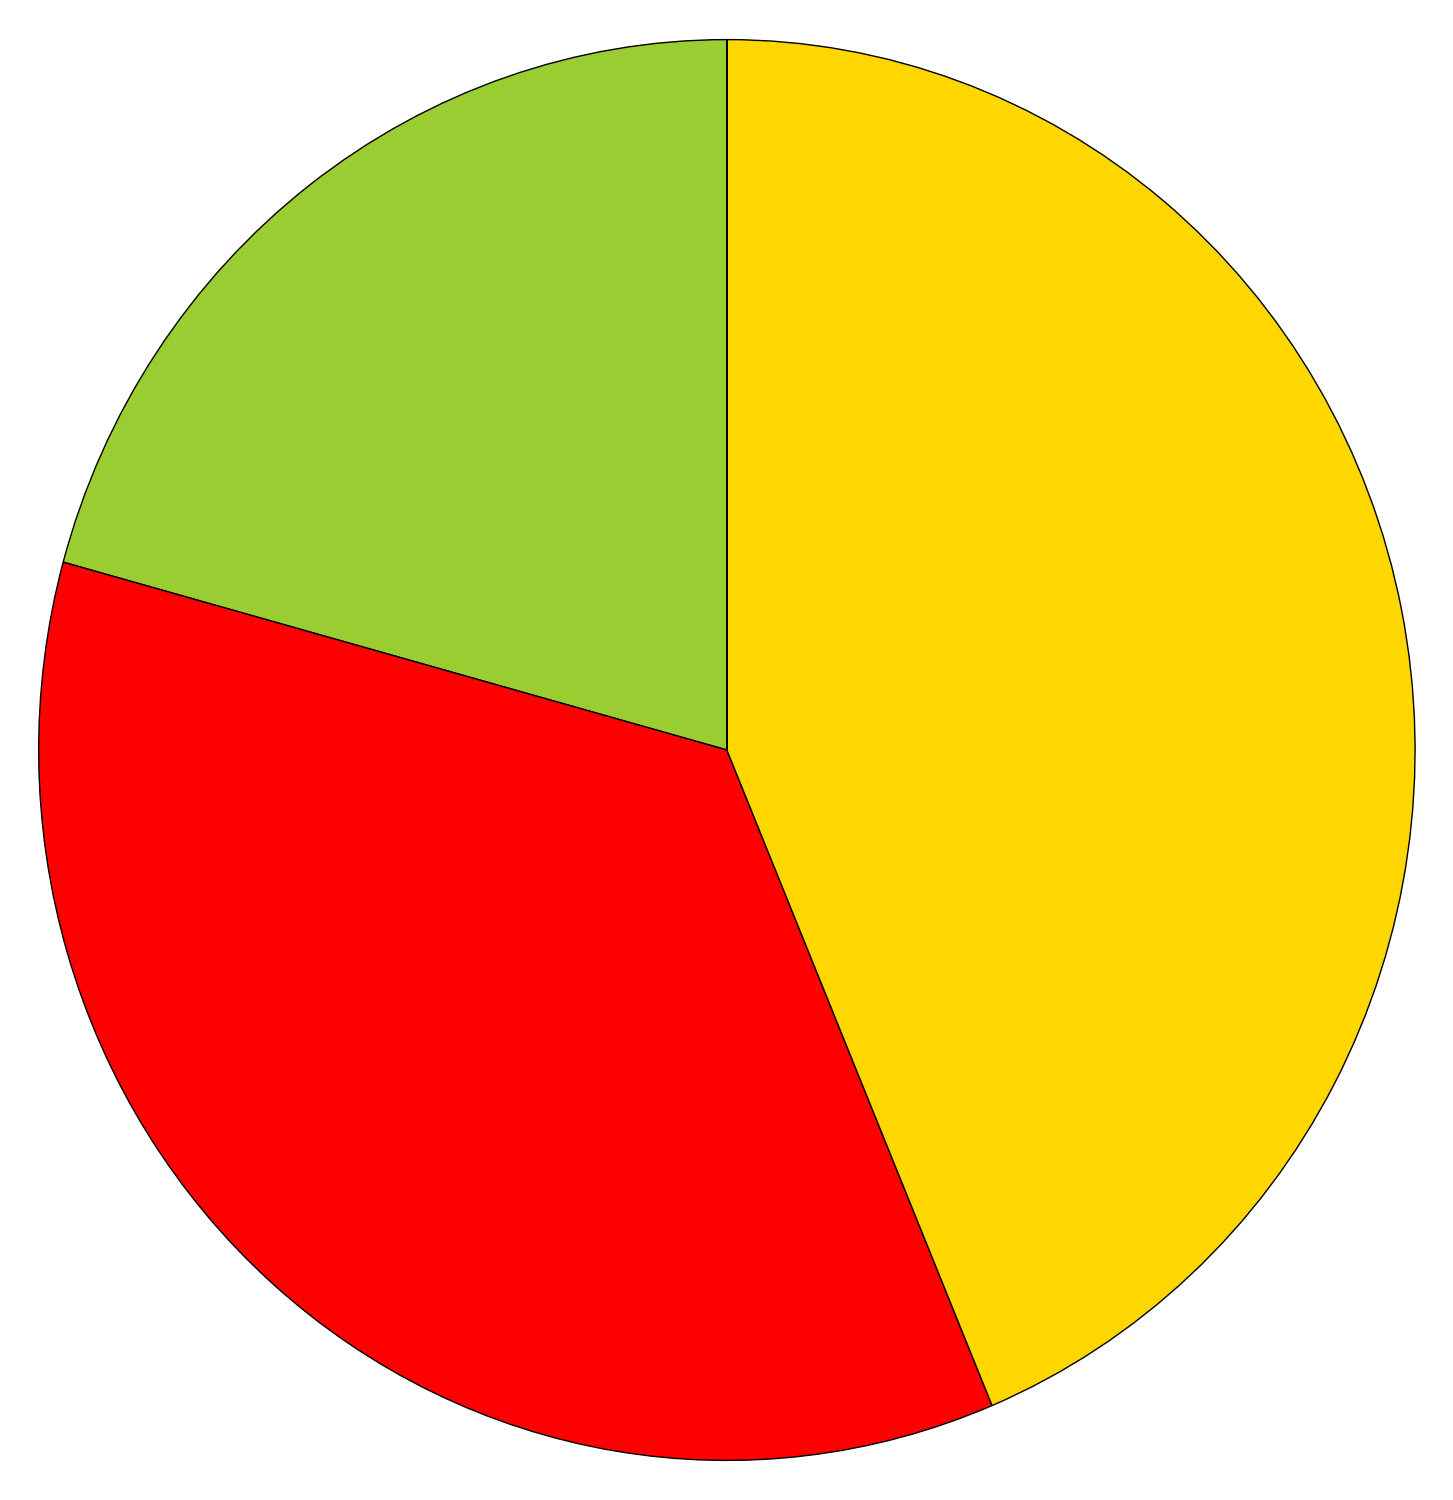
\includegraphics[width=\textwidth]{arousalEEGSVM}
    \caption{SVM}
  \end{subfigure}
  
  \begin{subfigure}[b]{0.3\textwidth}
    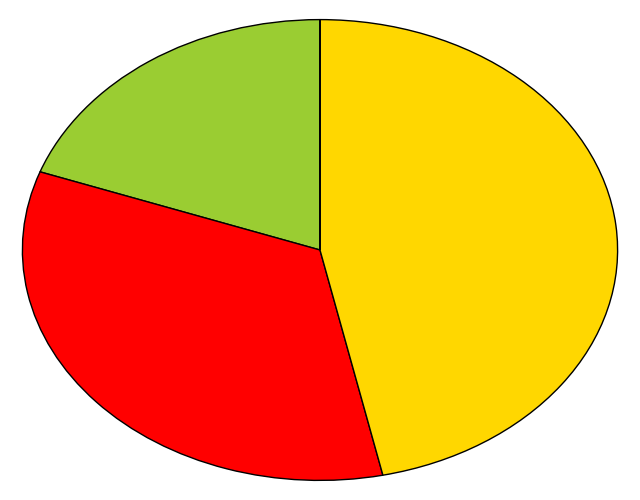
\includegraphics[width=\textwidth]{arousalEEGLDA}
    \caption{LDA}
  \end{subfigure}
  \hfill
  \begin{subfigure}[b]{0.3\textwidth}
    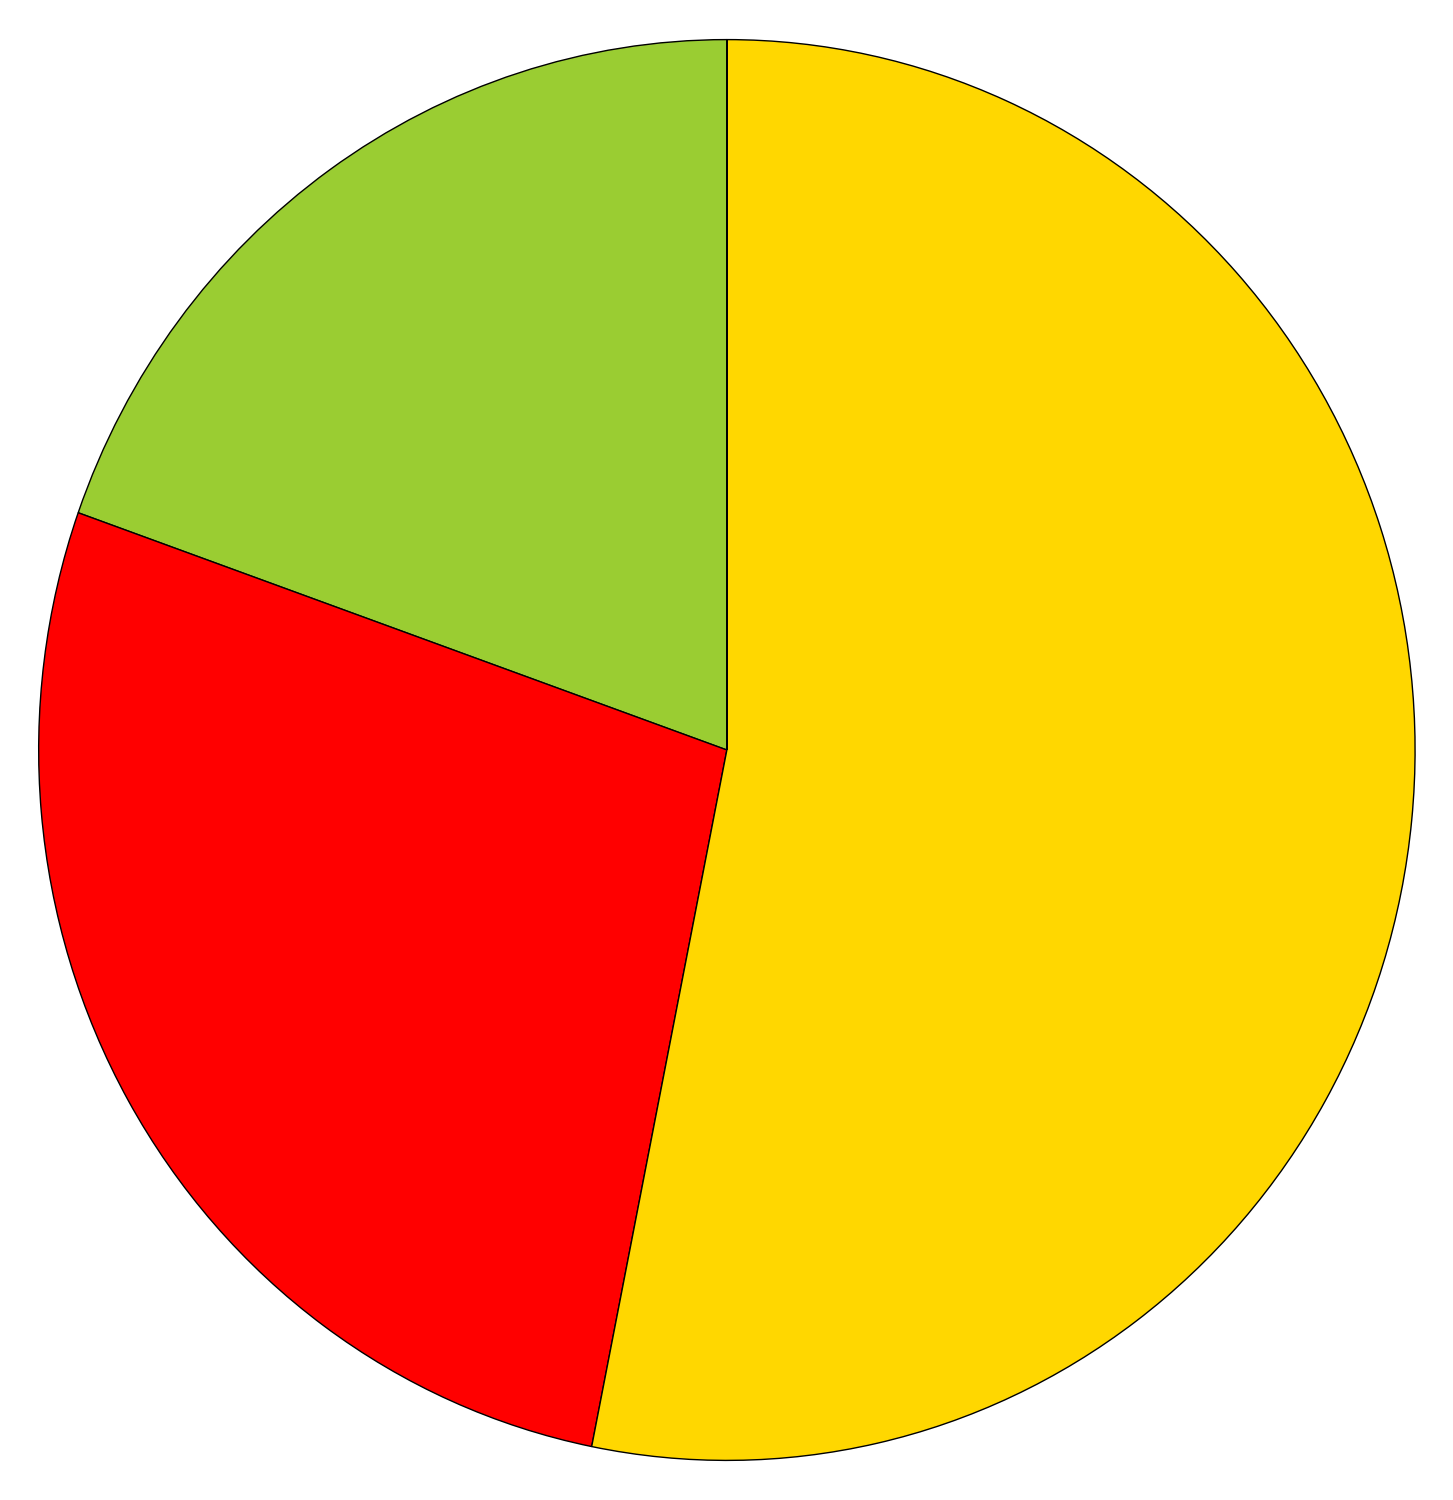
\includegraphics[width=\textwidth]{arousalEEGL1}
    \caption{Lasso regression}
  \end{subfigure}
  \hfill
  \begin{subfigure}[b]{0.3\textwidth}
    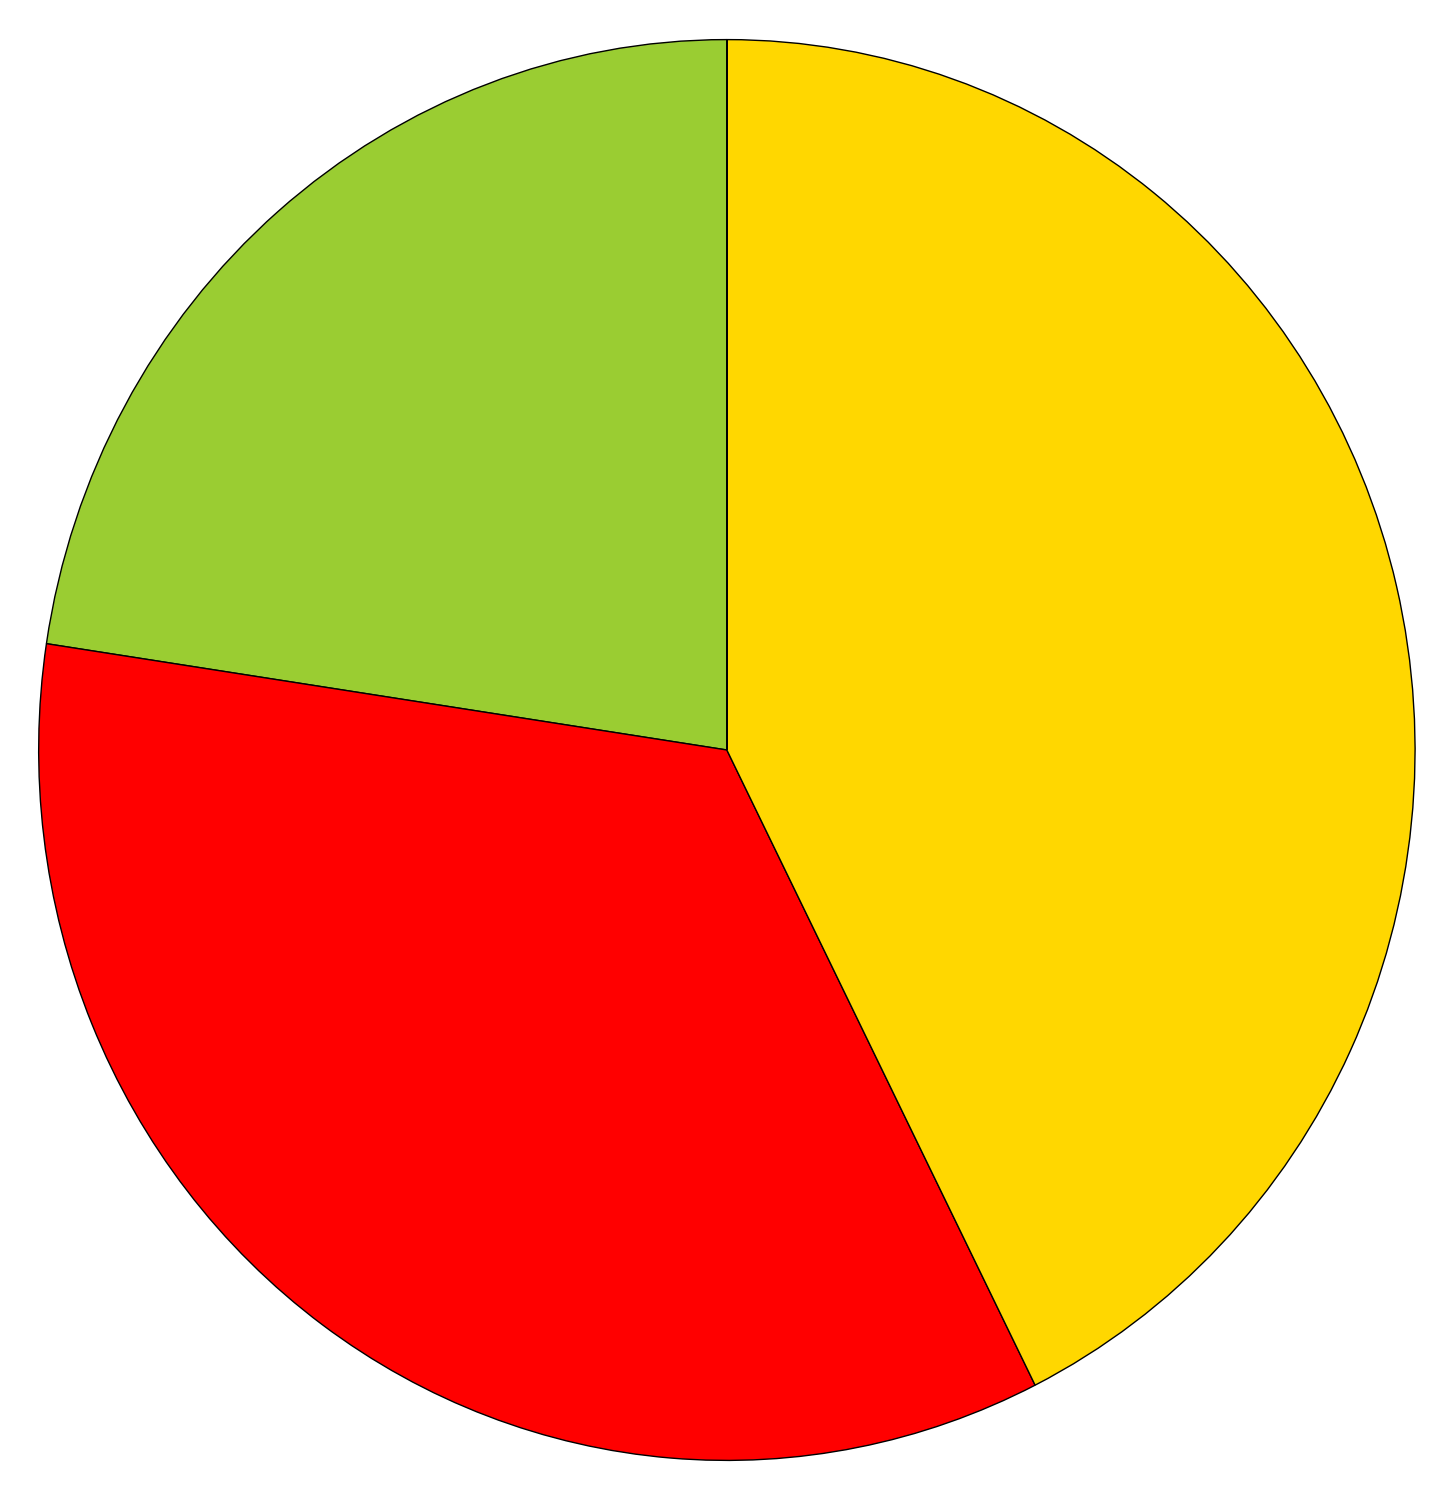
\includegraphics[width=\textwidth]{arousalEEGL2}
    \caption{Ridge regression}
  \end{subfigure}
  
  \begin{subfigure}[b]{0.3\textwidth}
    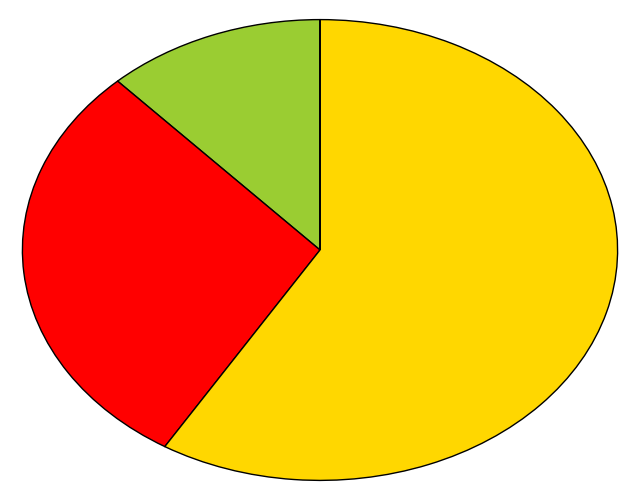
\includegraphics[width=\textwidth]{arousalEEGRF}
    \caption{Random forests}
  \end{subfigure}
  \hfill
  \begin{subfigure}[b]{0.3\textwidth}
    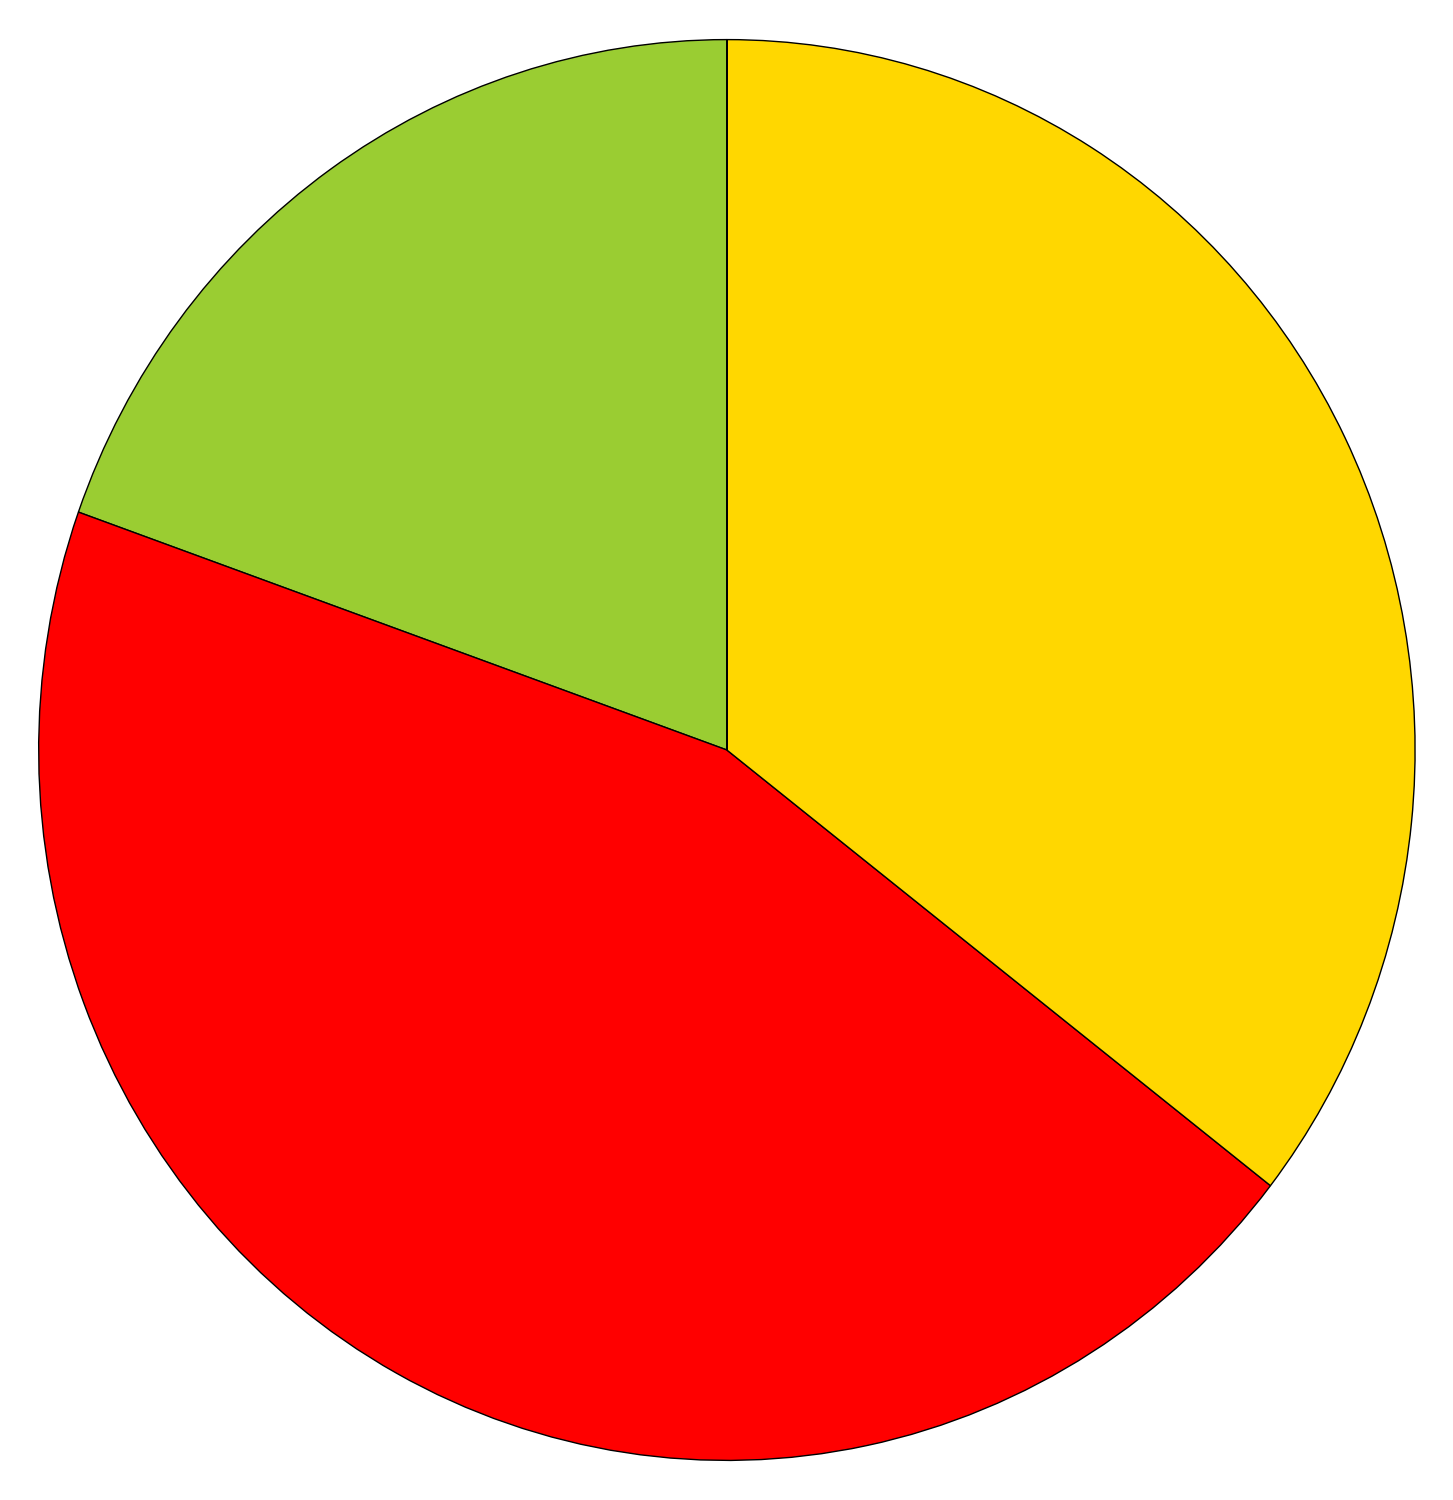
\includegraphics[width=\textwidth]{arousalEEGPCA}
    \caption{PCA}
  \end{subfigure}
  \hfill
  \begin{subfigure}[b]{0.3\textwidth}
    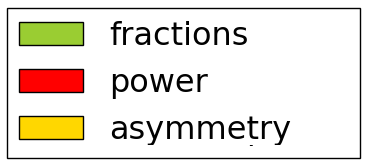
\includegraphics[width=\textwidth]{EEGlegend}
    \caption{Legend\label{arousalpiesEEGlegend}}
  \end{subfigure}
\caption{The distribution of the selected features for arousal classification of all persons combined of different feature selection methods. The feature set was limited to EEG features only.\label{arousalEEGpies}}
\end{figure}

\clearpage

\begin{figure}[!tbp]
  \centering
  \begin{subfigure}[b]{0.3\textwidth}
    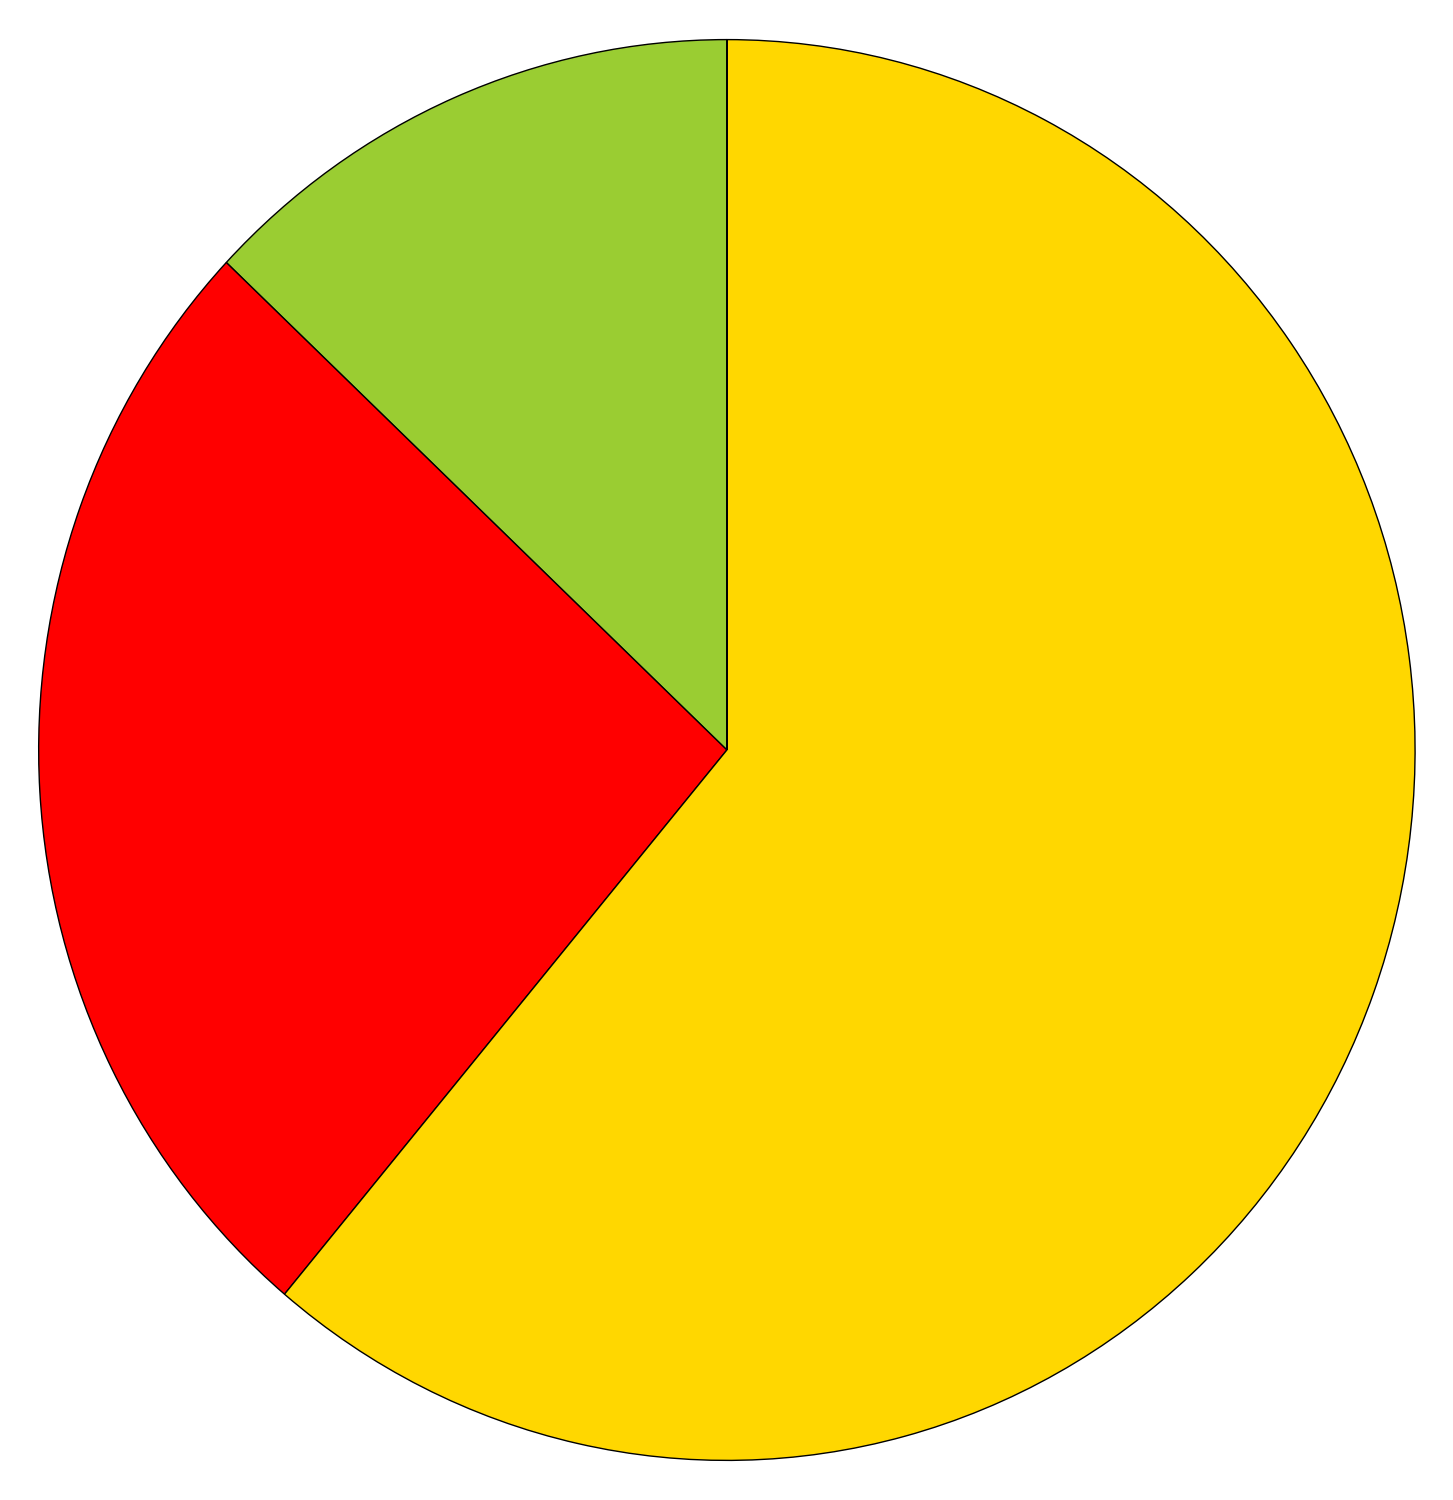
\includegraphics[width=\textwidth]{valenceEEGpearsonR}
    \caption{Pearson correlation}
  \end{subfigure}
  \hfill
  \begin{subfigure}[b]{0.3\textwidth}
    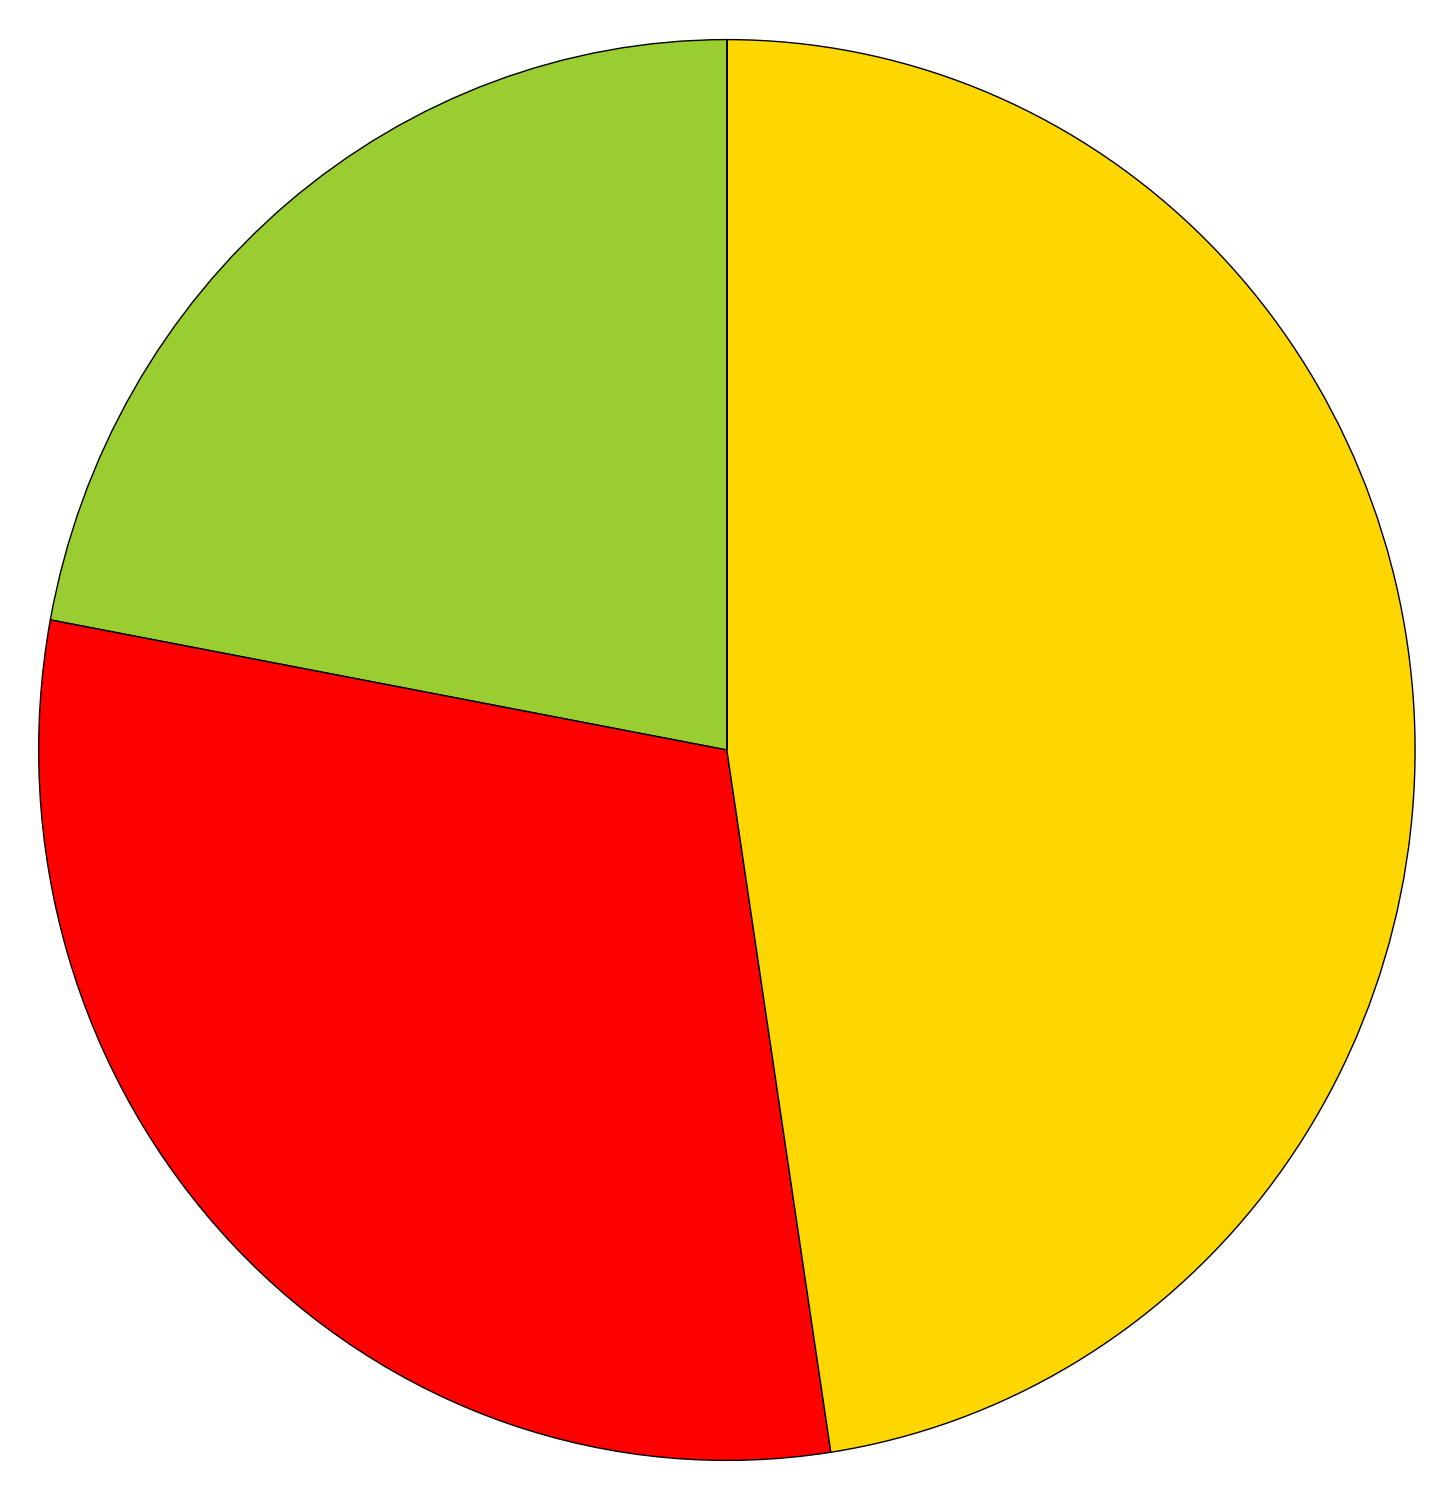
\includegraphics[width=\textwidth]{valenceEEGMutInf}
    \caption{Mutual information}
  \end{subfigure}
  \hfill
  \begin{subfigure}[b]{0.3\textwidth}
    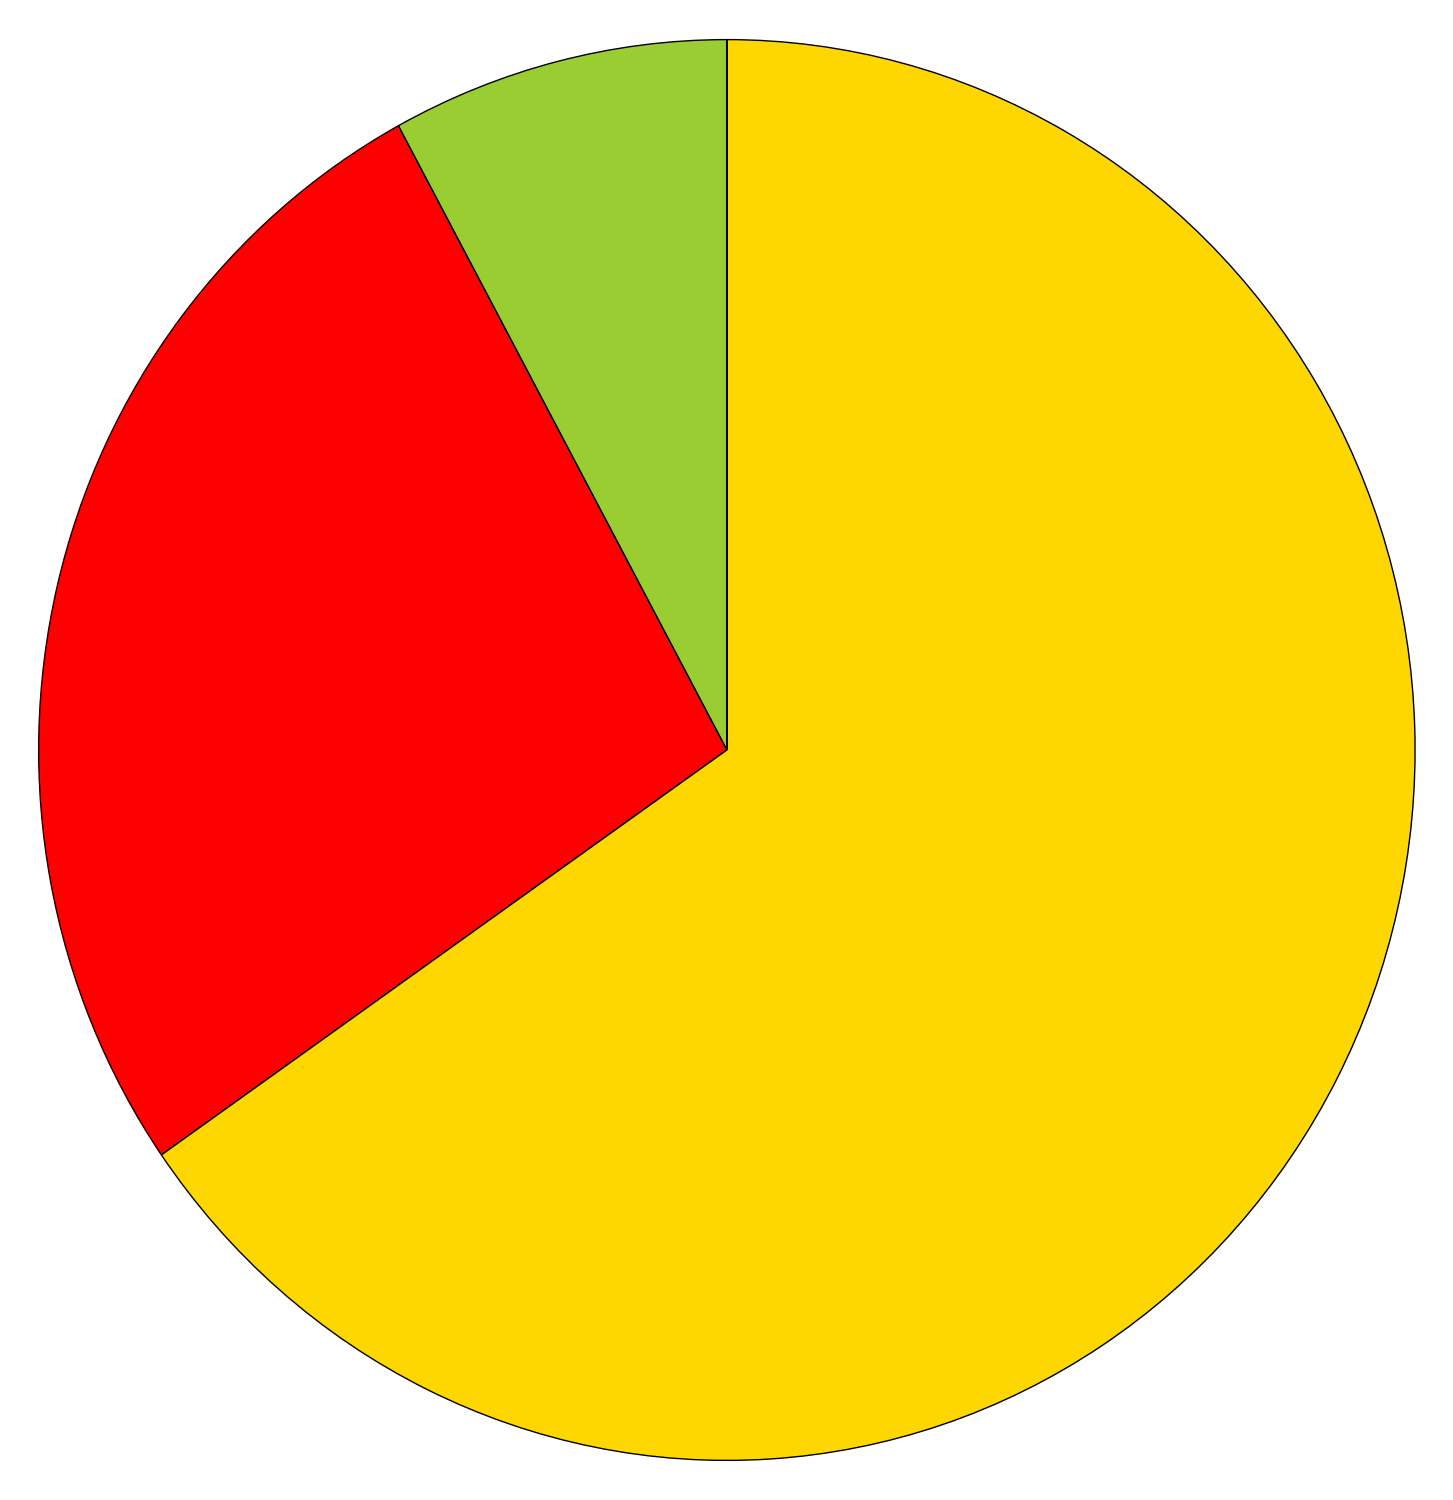
\includegraphics[width=\textwidth]{valenceEEGdCorr}
    \caption{Distance Correlation}
  \end{subfigure}
  
  \begin{subfigure}[b]{0.3\textwidth}
    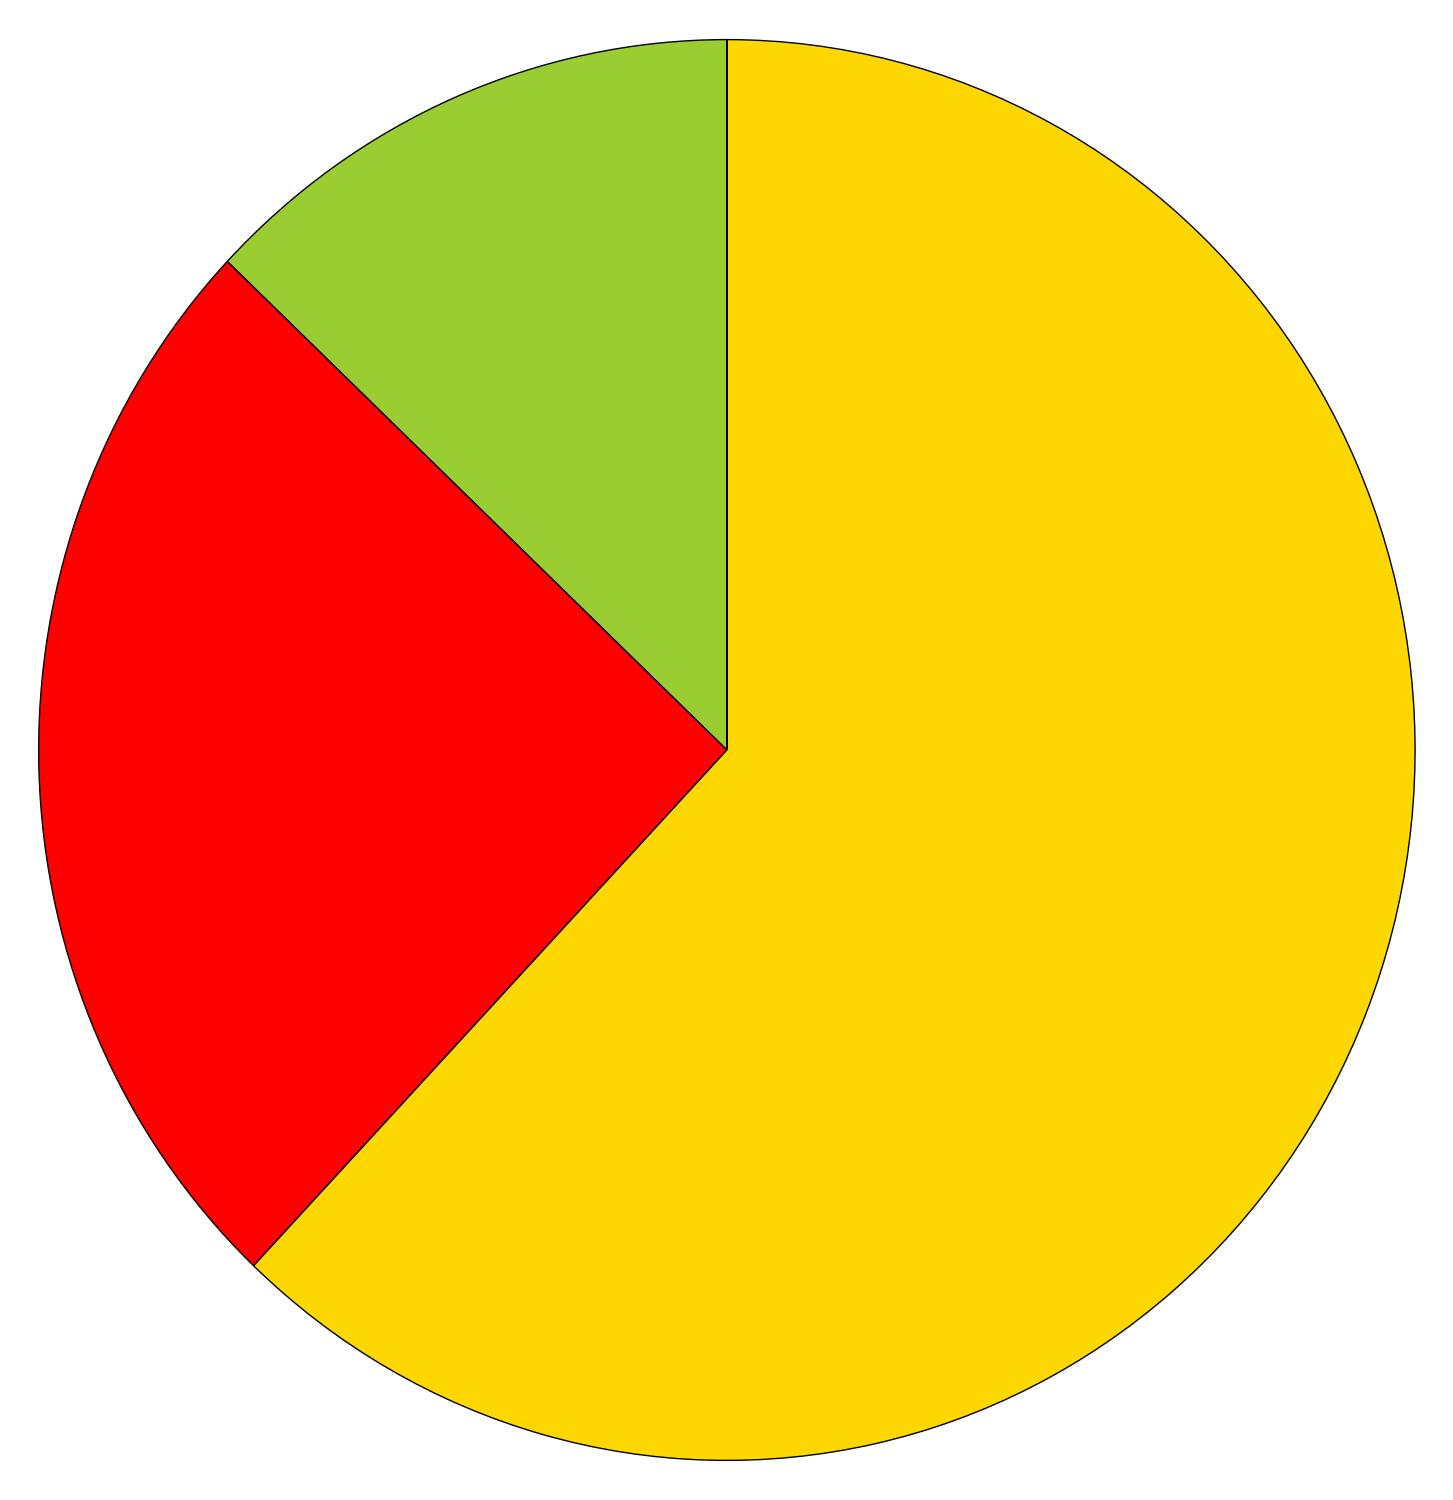
\includegraphics[width=\textwidth]{valenceEEGANOVA}
    \caption{ANOVA}
  \end{subfigure}
  \hfill
  \begin{subfigure}[b]{0.3\textwidth}
    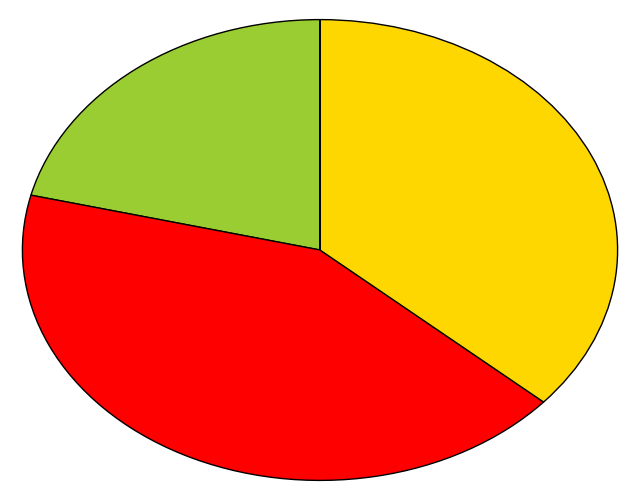
\includegraphics[width=\textwidth]{valenceEEGLR}
    \caption{Linear regression}
  \end{subfigure}
  \hfill
  \begin{subfigure}[b]{0.3\textwidth}
    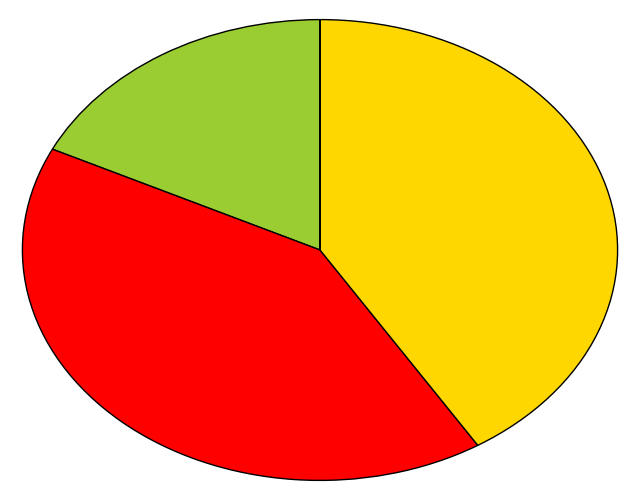
\includegraphics[width=\textwidth]{valenceEEGSVM}
    \caption{SVM}
  \end{subfigure}
  
  \begin{subfigure}[b]{0.3\textwidth}
    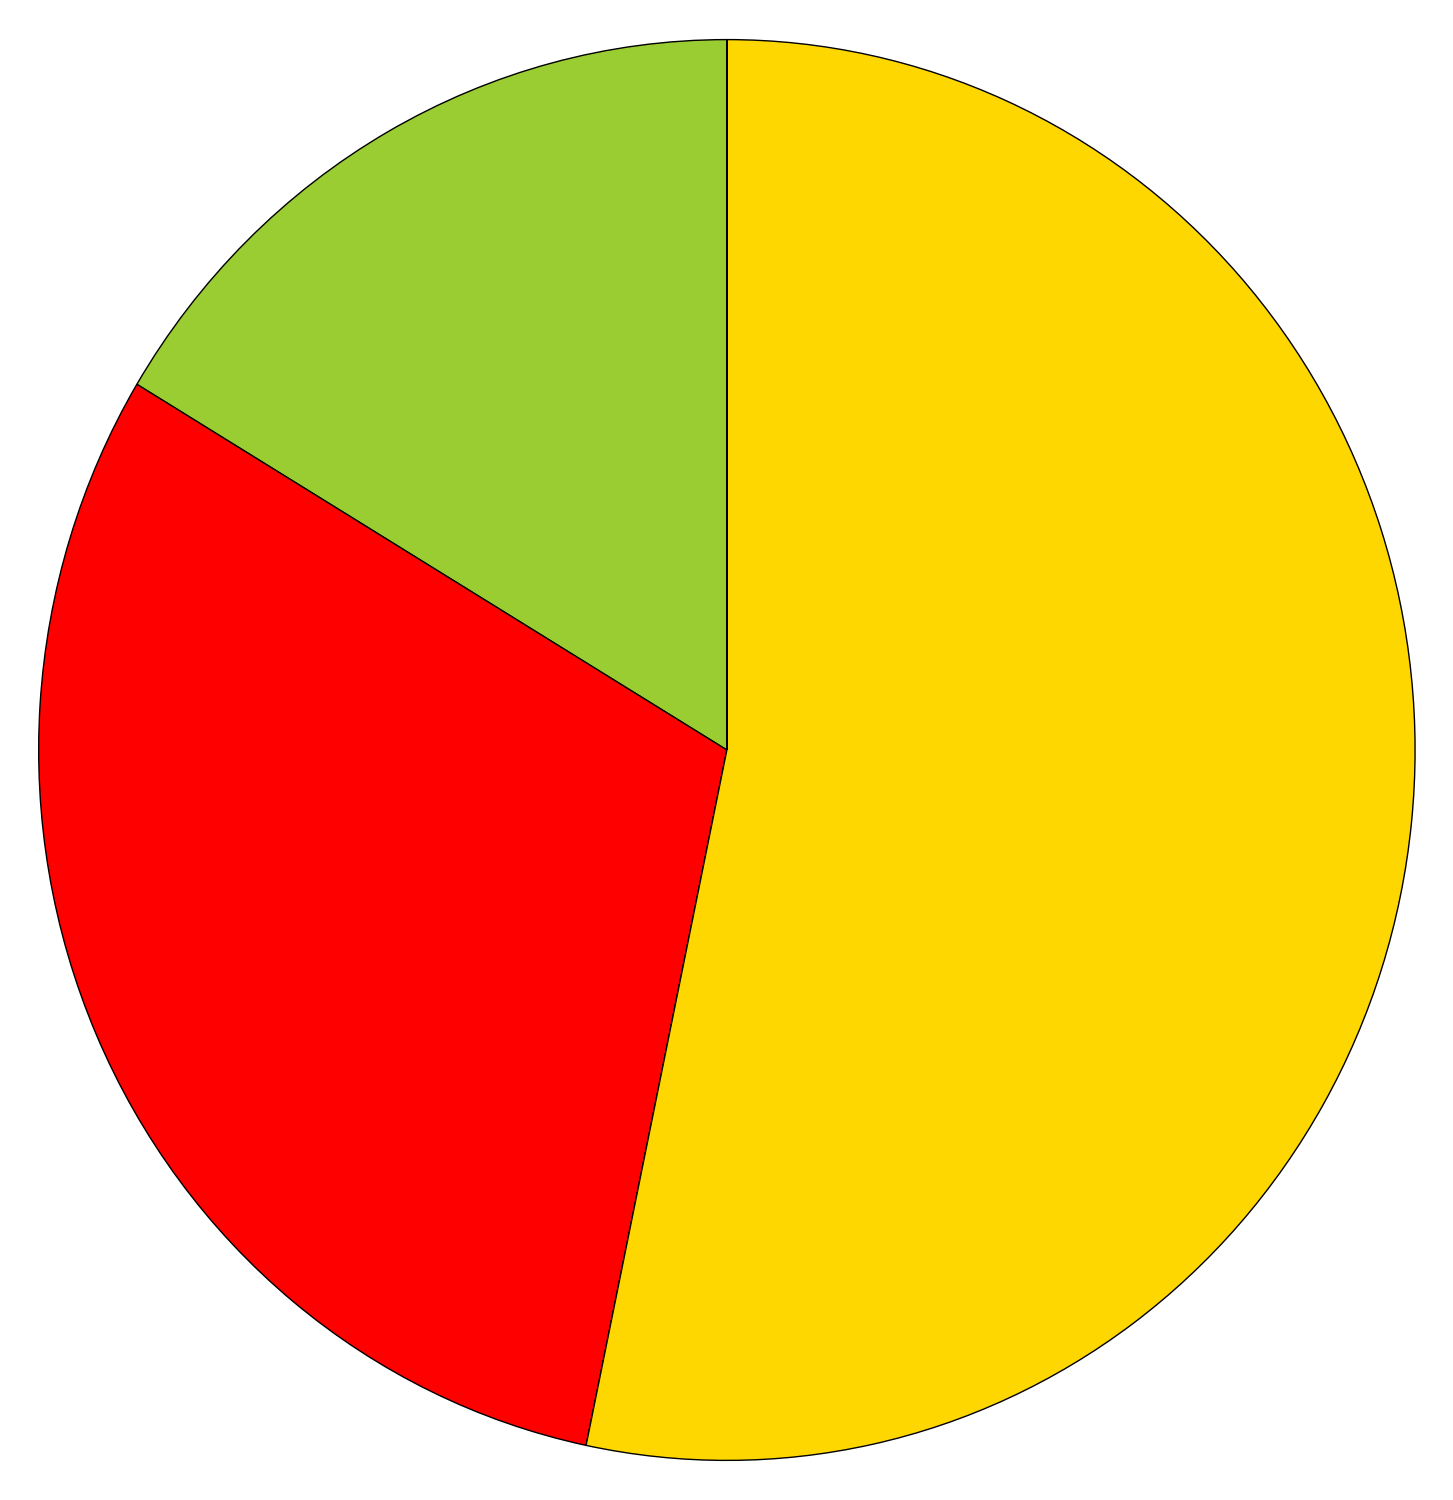
\includegraphics[width=\textwidth]{valenceEEGLDA}
    \caption{LDA}
  \end{subfigure}
  \hfill
  \begin{subfigure}[b]{0.3\textwidth}
    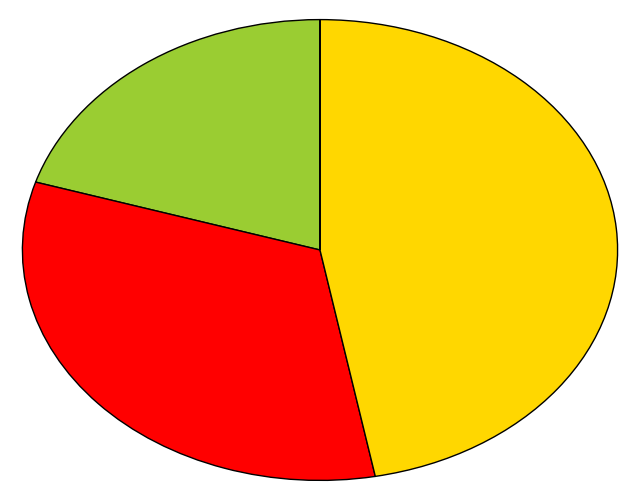
\includegraphics[width=\textwidth]{valenceEEGL1}
    \caption{Lasso regression}
  \end{subfigure}
  \hfill
  \begin{subfigure}[b]{0.3\textwidth}
    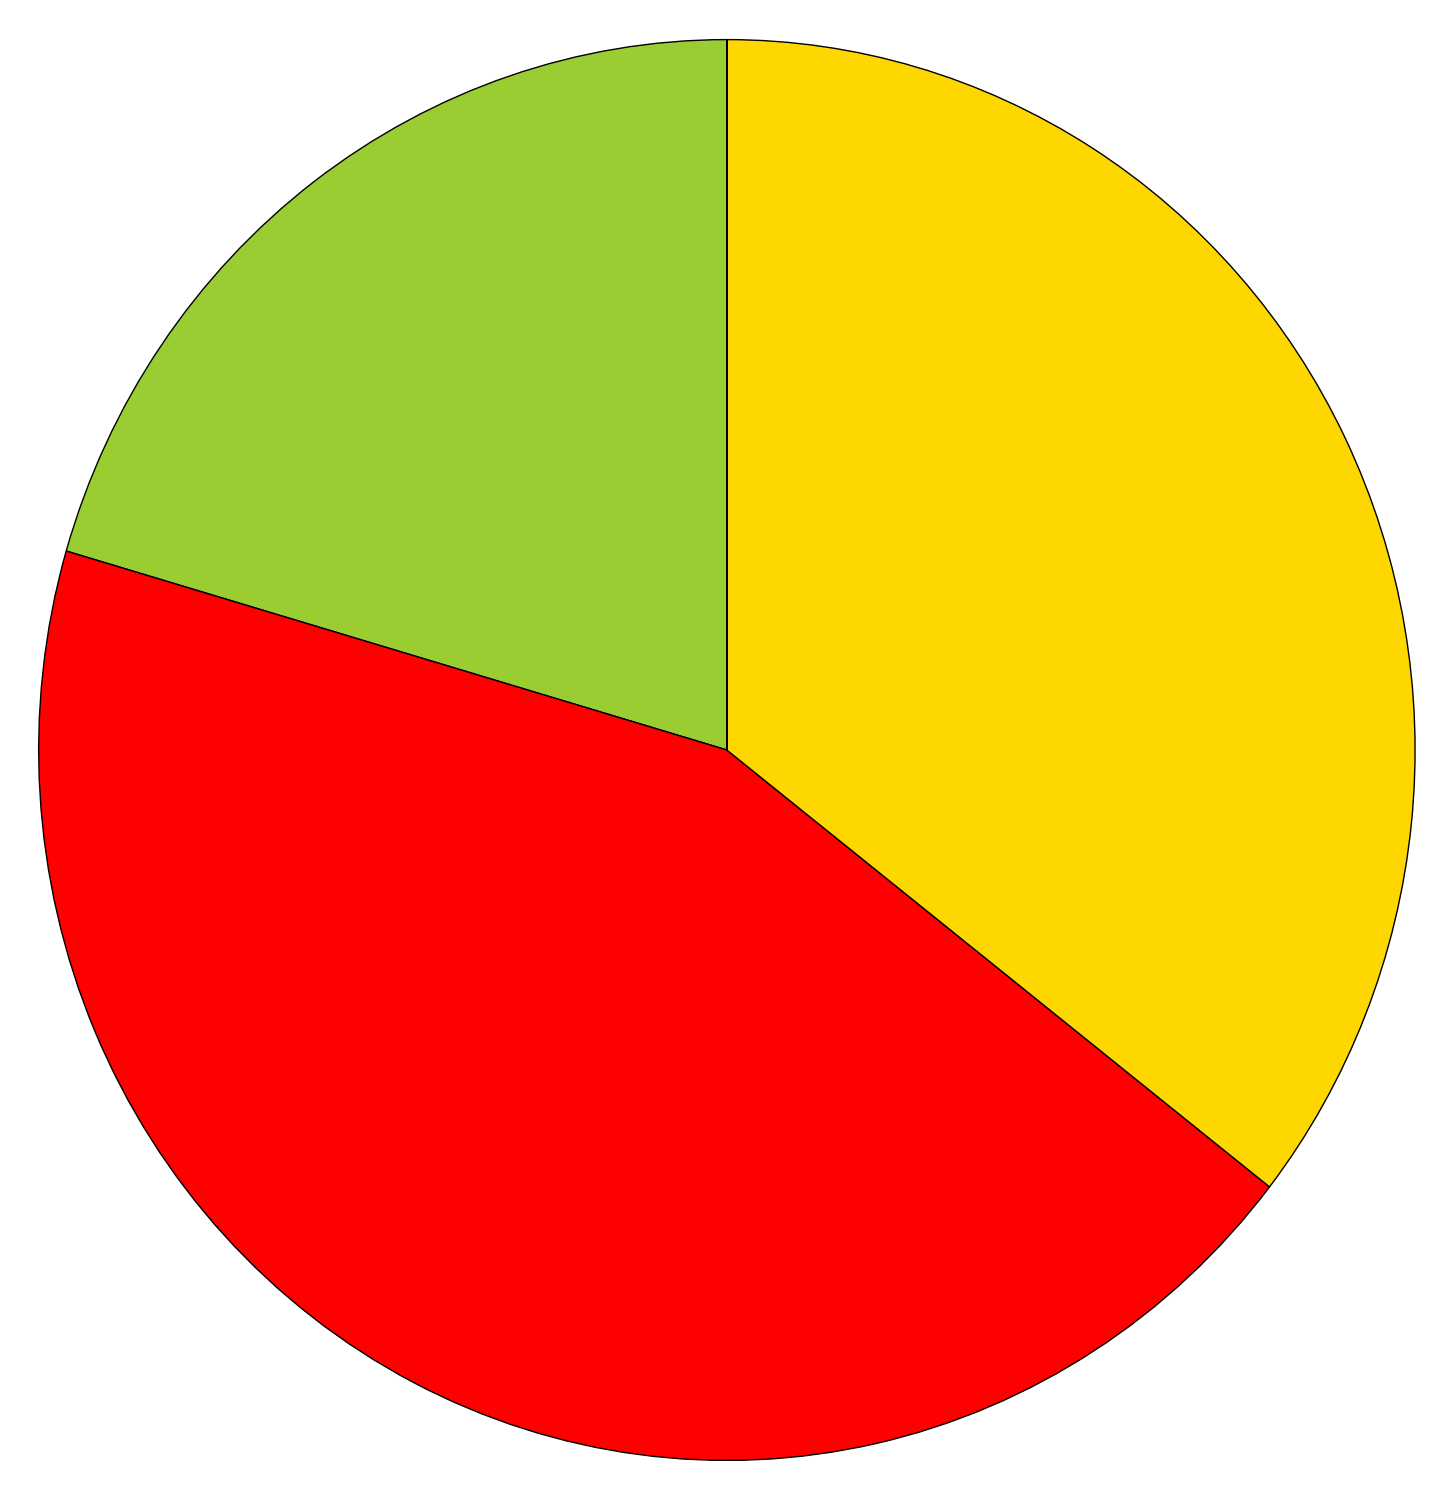
\includegraphics[width=\textwidth]{valenceEEGL2}
    \caption{Ridge regression}
  \end{subfigure}
  
  \begin{subfigure}[b]{0.3\textwidth}
    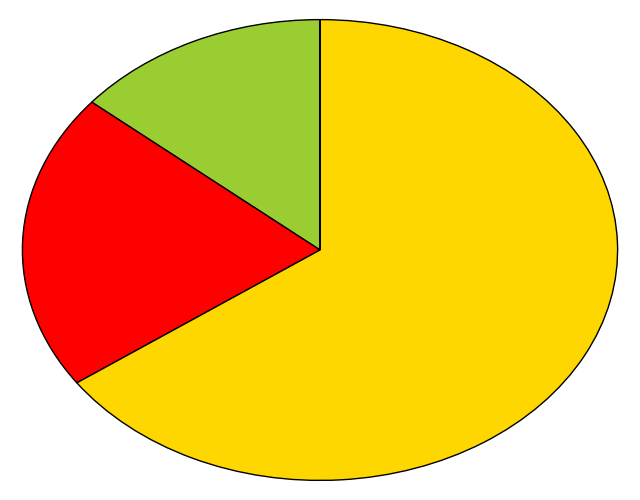
\includegraphics[width=\textwidth]{valenceEEGRF}
    \caption{Random forests}
  \end{subfigure}
  \hfill
  \begin{subfigure}[b]{0.3\textwidth}
    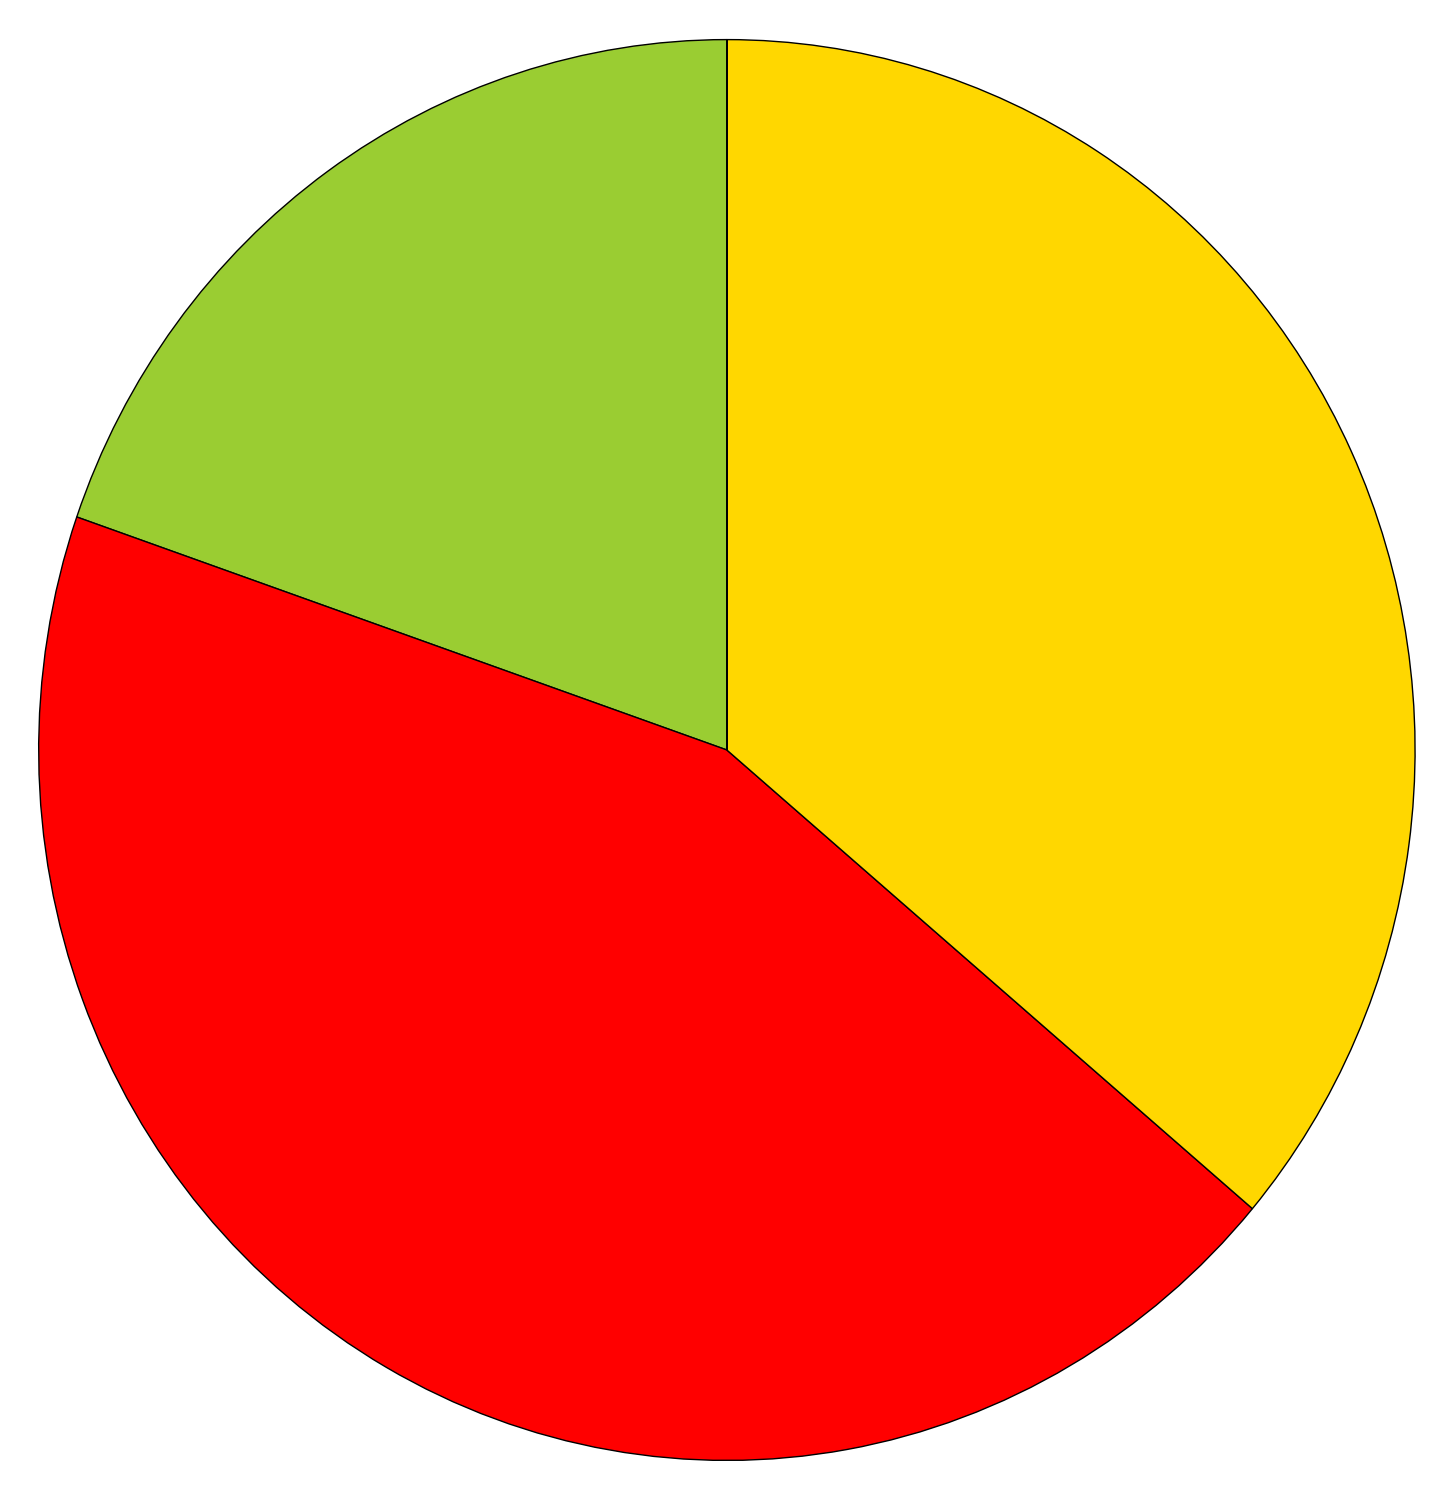
\includegraphics[width=\textwidth]{valenceEEGPCA}
    \caption{PCA}
  \end{subfigure}
  \hfill
  \begin{subfigure}[b]{0.3\textwidth}
    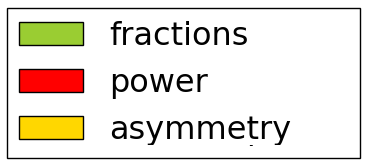
\includegraphics[width=\textwidth]{EEGlegend}
    \caption{Legend\label{valencepiesEEGlegend}}
  \end{subfigure}
  \caption{The distribution of the selected features for valence classification of all persons combined of different feature selection methods. The feature set was limited to EEG features only.\label{valenceEEGpies}}
\end{figure}
\clearpage

\begin{figure}[!tbp]
  \centering
  \begin{subfigure}[b]{0.3\textwidth}
    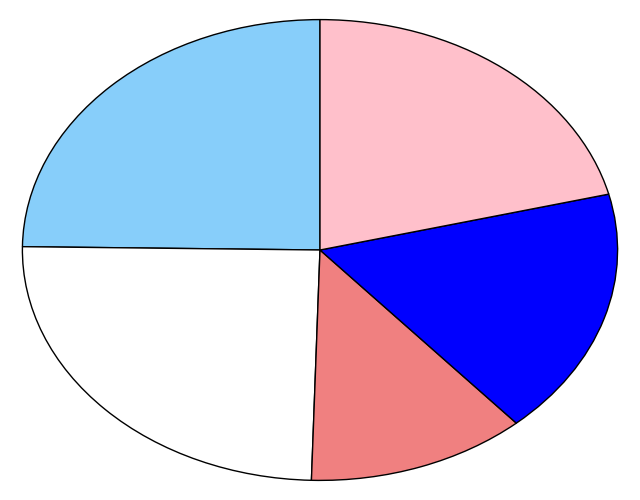
\includegraphics[width=\textwidth]{arousalnon-EEGpearsonR}
    \caption{Pearson correlation}
  \end{subfigure}
  \hfill
  \begin{subfigure}[b]{0.3\textwidth}
    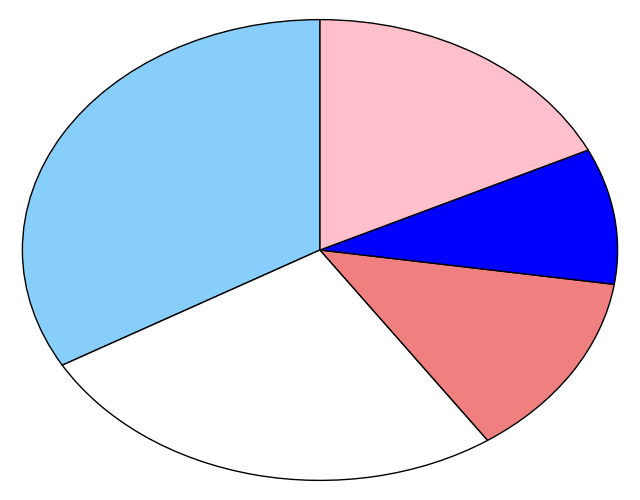
\includegraphics[width=\textwidth]{arousalnon-EEGMutInf}
    \caption{Mutual information}
  \end{subfigure}
  \hfill
  \begin{subfigure}[b]{0.3\textwidth}
    \includegraphics[width=\textwidth]{arousalnon-EEGdCorr}
    \caption{Distance Correlation}
  \end{subfigure}
  
  \begin{subfigure}[b]{0.3\textwidth}
    \includegraphics[width=\textwidth]{arousalnon-EEGANOVA}
    \caption{ANOVA}
  \end{subfigure}
  \hfill
  \begin{subfigure}[b]{0.3\textwidth}
    \includegraphics[width=\textwidth]{arousalnon-EEGLR}
    \caption{Linear regression}
  \end{subfigure}
  \hfill
  \begin{subfigure}[b]{0.3\textwidth}
    \includegraphics[width=\textwidth]{arousalnon-EEGSVM}
    \caption{SVM}
  \end{subfigure}
  
  \begin{subfigure}[b]{0.3\textwidth}
    \includegraphics[width=\textwidth]{arousalnon-EEGLDA}
    \caption{LDA}
  \end{subfigure}
  \hfill
  \begin{subfigure}[b]{0.3\textwidth}
    \includegraphics[width=\textwidth]{arousalnon-EEGL1}
    \caption{Lasso regression}
  \end{subfigure}
  \hfill
  \begin{subfigure}[b]{0.3\textwidth}
    \includegraphics[width=\textwidth]{arousalnon-EEGL2}
    \caption{Ridge regression}
  \end{subfigure}
  
  \begin{subfigure}[b]{0.3\textwidth}
    \includegraphics[width=\textwidth]{arousalnon-EEGRF}
    \caption{Random forests}
  \end{subfigure}
  \hfill
  \begin{subfigure}[b]{0.3\textwidth}
    \includegraphics[width=\textwidth]{arousalnon-EEGPCA}
    \caption{PCA}
  \end{subfigure}
  \hfill
  \begin{subfigure}[b]{0.3\textwidth}
    \includegraphics[width=\textwidth]{non-EEGlegend}
    \caption{Legend\label{arousalpiesnon-EEGlegend}}
  \end{subfigure}    
\caption{The distribution of the selected features for arousal classification of all persons combined of different feature selection methods. The feature set was limited to non-EEG features only.\label{arousalnon-EEGpies}}
\end{figure}

\clearpage

\begin{figure}[!tbp]
  \centering
  \begin{subfigure}[b]{0.3\textwidth}
    \includegraphics[width=\textwidth]{valencenon-EEGpearsonR}
    \caption{Pearson correlation}
  \end{subfigure}
  \hfill
  \begin{subfigure}[b]{0.3\textwidth}
    \includegraphics[width=\textwidth]{valencenon-EEGMutInf}
    \caption{Mutual information}
  \end{subfigure}
  \hfill
  \begin{subfigure}[b]{0.3\textwidth}
    \includegraphics[width=\textwidth]{valencenon-EEGdCorr}
    \caption{Distance Correlation}
  \end{subfigure}
  
  \begin{subfigure}[b]{0.3\textwidth}
    \includegraphics[width=\textwidth]{valencenon-EEGANOVA}
    \caption{ANOVA}
  \end{subfigure}
  \hfill
  \begin{subfigure}[b]{0.3\textwidth}
    \includegraphics[width=\textwidth]{valencenon-EEGLR}
    \caption{Linear regression}
  \end{subfigure}
  \hfill
  \begin{subfigure}[b]{0.3\textwidth}
    \includegraphics[width=\textwidth]{valencenon-EEGSVM}
    \caption{SVM}
  \end{subfigure}
  
  \begin{subfigure}[b]{0.3\textwidth}
    \includegraphics[width=\textwidth]{valencenon-EEGLDA}
    \caption{LDA}
  \end{subfigure}
  \hfill
  \begin{subfigure}[b]{0.3\textwidth}
    \includegraphics[width=\textwidth]{valencenon-EEGL1}
    \caption{Lasso regression}
  \end{subfigure}
  \hfill
  \begin{subfigure}[b]{0.3\textwidth}
    \includegraphics[width=\textwidth]{valencenon-EEGL2}
    \caption{Ridge regression}
  \end{subfigure}
  
  \begin{subfigure}[b]{0.3\textwidth}
    \includegraphics[width=\textwidth]{valencenon-EEGRF}
    \caption{Random forests}
  \end{subfigure}
  \hfill
  \begin{subfigure}[b]{0.3\textwidth}
    \includegraphics[width=\textwidth]{valencenon-EEGPCA}
    \caption{PCA}
  \end{subfigure}
  \hfill
  \begin{subfigure}[b]{0.3\textwidth}
    \includegraphics[width=\textwidth]{non-EEGlegend}
    \caption{Legend\label{valencepiesnon-EEGlegend}}
  \end{subfigure}
  \caption{The distribution of the selected features for valence classification of all persons combined of different feature selection methods. The feature set was limited to non-EEG features only.\label{valencenon-EEGpies}}
\end{figure}
\clearpage

\section{Important EEG channels}

Another component of this work is to dig into the EEG features and find out which channels are most important. This was done by taking the Random forest as a feature selection model and looking and building a model with EEG features only. From this model, the selected features were taken and the occurrences of each EEG channel were counted. These frequencies were used as weights to create the following topoplots in Figure \ref{arousalchannel} and Figure \ref{valencechannel}.

\begin{figure}[H]
\centering
  \begin{subfigure}[b]{.4\textwidth}
    \includegraphics[width=\textwidth]{arousal_psd.eps}
    \caption{The occurences of the selected channels for arousal classification. The model seems to use channels all over the brain, with channel FC2.\label{arousalchannel}}
  \end{subfigure}
\hfill
  \begin{subfigure}[b]{.4\textwidth}
    \includegraphics[width=\textwidth]{valence_psd.eps}
    \caption{The occurences of the selected channels for valence classification. The model seems to give most weight to frontal channels.\label{valencechannel}}
  \end{subfigure}
\end{figure}


Looking at the topoplots depicted in Figure \ref{arousalchannel} for arousal and Figure \ref{valencechannel} for valence, one can see that for arousal, no clear region is used. Channel Fc2 has the largest weight, combined with some importance for the channels at the outer left side of the scalp. For valence, most of the importances is located in the frontal channels, which concurs with results of similar research in literature. 

\npar

The same can be done for the asymmetry features, here a distinction was made between DASM and RASM features on one hand and the DCAU and RCAU features on the other hand. Again, occurrences were counted and topoplots were created.

\begin{figure}[H]
\centering
  \begin{subfigure}[b]{.4\textwidth}
    \includegraphics[width=\textwidth]{arousal_asym.eps}
    \caption{The occurences of the selected DASM and RASM channel pairs for arousal classification. The model seems to focus on frontal EEG channels.\label{arousal_asym}}
  \end{subfigure}
\hfill
  \begin{subfigure}[b]{.4\textwidth}
    \includegraphics[width=\textwidth]{valence_asym.eps}
    \caption{The occurences of the selected DASM and RASM channel pairs for valence classification. The model seems to focus on frontal EEG channels.\label{valence_asym}}
  \end{subfigure}
\end{figure}

The DASM and RASM features are depicted in Figure \ref{arousal_asym} and Figure \ref{valence_asym} for arousal and valence respectively. It is clear that the asymmetry should be measured at the front of the scalp for both arousal and valence. Some importance can be found at the center and back of the scalp though, albeit limited.

\npar

The DCAU and RCAU features are depicted in Figure \ref{arousal_dcau} and Figure \ref{valence_dcau} for arousal and valence respectively. Arousal seems to use frontal left EEG channels combined with some center right EEG channel pairs. For valence, the opposite is true, the frontal right EEG channels are used in combination with the left center EEG channel pairs.

\begin{figure}[H]
\centering
  \begin{subfigure}[b]{.4\textwidth}
    \includegraphics[width=\textwidth]{arousal_dcau}
    \caption{Origin of the asymmetry features for arousal classification.\label{arousal_dcau}}
  \end{subfigure}
\hfill
  \begin{subfigure}[b]{.4\textwidth}
    \includegraphics[width=\textwidth]{valence_dcau}
    \caption{Origin of the asymmetry features for valence classification.\label{valence_dcau}}
  \end{subfigure}
\end{figure}

\section{Stability}
Random forests have the disadvantage that they have an element of randomness, meaning that they might not always select the same features, making them potentially unstable. It is possible to make the random forest algorithm more stable, by adding additional trees or running the algorithm several times and averaging the importance values. 

\npar

One way to measure the stability is to run the algorithm twice and look at the similarity of the selected features. The similarity can be calculated using the Jaccard index, as explained in Section \ref{jaccard}. In this work, the importances of the random forest features selection were averaged over 30 runs to ensure stability. The Jaccard index was measured for different values of the 'runs' parameter for each person. The average and standard deviation over all persons is shown in Table \ref{specificJaccard}.

\begin{table}[H]
\centering
\caption{The Jaccard index of two consecutive features sets for the random forest feature selection method. The indexes are averaged over all persons.\label{specificJaccard}}
\begin{tabular}{l|l|ll}
\textbf{What} & \textbf{runs} & \textbf{Average Jaccard index} & \textbf{STD Jaccard index} \\ \hline
valence       & 1             & 0.83021                   & 0.20581               \\
valence       & 5             & 0.64683                   & 0.21850               \\
valence       & 10            & 0.63963                   & 0.24620               \\
valence       & 20            & 0.66682                   & 0.25415               \\
valence       & 30            & 0.74313                   & 0.24272               \\
valence       & 40            & 0.77958                   & 0.22432               \\
valence       & 50            & 0.76278                   & 0.24394               \\ \hline
arousal       & 1             & 0.83318                   & 0.18140               \\
arousal       & 5             & 0.61578                   & 0.27061               \\
arousal       & 10            & 0.70878                   & 0.24949               \\
arousal       & 20            & 0.70873                   & 0.24849               \\
arousal       & 30            & 0.79145                   & 0.24380               \\
arousal       & 40            & 0.77422                   & 0.21200               \\
arousal       & 50            & 0.76370                   & 0.22673              
\end{tabular}
\end{table}

Looking at Table \ref{specificJaccard}, the Jaccard index is less stable, meaning that its values changes rapidly between 1 and 5 runs. This might be due to the fact that importance values are estimated a limited number of times. When the random forest feature selection uses importance values, averaged over 30 runs, the value of the Jaccard index become more or less stable, around 0.75-0.77. One thing to keep in mind though is that the standard deviation of 0.2-0.25 is quite large, which means that the stability of the RF method varies from person to person.